\documentclass{ximera}
%
%%% Begin Laad packages
%
\makeatletter
\@ifclassloaded{xourse}{%
    \typeout{Start loading preamble.tex (in a XOURSE)}%
    \def\isXourse{true}   % automatically defined; pre 112022 it had to be set 'manually' in a xourse
}{%
    \typeout{Start loading preamble.tex (NOT in a XOURSE)}%
}
\makeatother

\pgfplotsset{compat=1.16}

\usepackage{currfile}

% 201908/202301: PAS OP: babel en doclicense lijken problemen te veroorzaken in .jax bestand
% (wegens syntax error met toegevoegde \newcommands ...)
\pdfOnly{
    \usepackage[hyperxmp=false,type={CC},modifier={by-nc-sa},version={4.0}]{doclicense}
    \usepackage[dutch]{babel}
}


\usepackage[utf8]{inputenc}
\usepackage{morewrites}   % nav zomercursus (answer...?)
\usepackage{multirow}
\usepackage{multicol}
\usepackage{tikzsymbols}
\usepackage{tikz-3dplot}
\usepackage{ifthen}
%\usepackage{animate} BREAKS HTML STRUCTURE USED BY XIMERA
\usepackage{relsize}

\usepackage{eurosym}    % \euro  (€ werkt niet in xake ...?)
\usepackage{wrapfig}

\usepackage{cancel}

\usepackage{tabularx}
% Nuttig als ook interactieve beamer slides worden voorzien:
\providecommand{\p}{} % default nothing ; potentially usefull for slides: redefine as \pause
%providecommand{\p}{\pause}

\usepackage{caption} % captionof
%\usepackage{pdflscape}    % landscape environment

% Met "\newcommand\showtodonotes{}" kan je todonotes tonen (in pdf/online)
% 201908: online werkt het niet (goed)
\providecommand\showtodonotes{disable}
\providecommand\todo[1]{\typeout{TODO #1}}
%\usepackage[\showtodonotes]{todonotes}
%\usepackage{todonotes}

%
% Poging tot aanpassen layout
%
\usepackage{tcolorbox}
\tcbuselibrary{theorems}

%%% Einde laad packages

%%% Begin Ximera specifieke zaken

% \graphicspath{
% 	{../../}
% 	{../}
% 	{./}
%   	{../../pictures/}
%    	{../pictures/}
%    	{./pictures/}
% 	{./explog/}    % M05 in groeimodellen       
% }

%%% Einde Ximera specifieke zaken

%
% define softer blue/red/green, use KU Leuven base colors for blue (and dark orange for red ?)
%
% todo: rather redefine blue/red/green ...?
%\definecolor{xmblue}{rgb}{0.01, 0.31, 0.59}
%\definecolor{xmred}{rgb}{0.89, 0.02, 0.17}
\definecolor{xmdarkblue}{rgb}{0.122, 0.671, 0.835}   % KU Leuven Blauw
\definecolor{xmblue}{rgb}{0.114, 0.553, 0.69}        % KU Leuven Blauw
\definecolor{xmgreen}{rgb}{0.13, 0.55, 0.13}         % No KULeuven variant for green found ...

\definecolor{xmaccent}{rgb}{0.867, 0.541, 0.18}      % KU Leuven Accent (orange ...)
\definecolor{kuaccent}{rgb}{0.867, 0.541, 0.18}      % KU Leuven Accent (orange ...)

\colorlet{xmred}{xmaccent!50!black}                  % Darker version of KU Leuven Accent

\providecommand{\blue}[1]{{\color{blue}#1}}    
\providecommand{\red}[1]{{\color{red}#1}}

\renewcommand\CancelColor{\color{xmaccent!50!black}}

% werkt in math en text mode om MATH met oranje (of grijze...)  achtergond te tonen (ook \important{\text{blabla}} lijkt te werken)
%\newcommand{\important}[1]{\ensuremath{\colorbox{xmaccent!50!white}{$#1$}}}   % werkt niet in Mathjax
%\newcommand{\important}[1]{\ensuremath{\colorbox{lightgray}{$#1$}}}
%\newcommand{\important}[1]{\ensuremath{\colorbox{orange}{$#1$}}}   % TODO: kleur aanpassen voor mathjax; wordt overschreven infra!
\newcommand{\important}[1]{\ensuremath{\fcolorbox{black}{white}{$#1$}}}


% Uitzonderlijk kan met \pdfnl in de PDF een newline worden geforceerd, die online niet nodig/nuttig is omdat daar de regellengte hoe dan ook niet gekend is.
\ifdefined\HCode%
\providecommand{\pdfnl}{}%
\else%
\providecommand{\pdfnl}{%
  \\%
}%
\fi

% Uitzonderlijk kan met \handoutnl in de handout-PDF een newline worden geforceerd, die noch online noch in de PDF-met-antwoorden nuttig is.
\ifdefined\HCode
\providecommand{\handoutnl}{}
\else
\providecommand{\handoutnl}{%
\ifhandout%
  \nl%
\fi%
}
\fi



% \cellcolor IGNORED by tex4ht ?
% \begin{center} seems not to wordk
    % (missing margin-left: auto;   on tabular-inside-center ???)
%\newcommand{\importantcell}[1]{\ensuremath{\cellcolor{lightgray}#1}}  %  in tabular; usablility to be checked
\providecommand{\importantcell}[1]{\ensuremath{#1}}     % no mathjax2 support for colloring array cells

\pdfOnly{
  \renewcommand{\important}[1]{\ensuremath{\colorbox{kuaccent!50!white}{$#1$}}}
  \renewcommand{\importantcell}[1]{\ensuremath{\cellcolor{kuaccent!40!white}#1}}   
}

%%% Tikz styles


\pgfplotsset{compat=1.16}

\usetikzlibrary{trees,positioning,arrows,fit,shapes,math,calc,decorations.markings,through,intersections,patterns,matrix}

\usetikzlibrary{decorations.pathreplacing,backgrounds}    % 5/2023: from experimental


\usetikzlibrary{angles,quotes}

\usepgfplotslibrary{fillbetween} % bepaalde_integraal
\usepgfplotslibrary{polar}    % oa voor poolcoordinaten.tex

\pgfplotsset{ownstyle/.style={axis lines = center, axis equal image, xlabel = $x$, ylabel = $y$, enlargelimits}} 

\pgfplotsset{
	plot/.style={no marks,samples=50}
}

\newcommand{\xmPlotsColor}{
	\pgfplotsset{
		plot1/.style={darkgray,no marks,samples=100},
		plot2/.style={lightgray,no marks,samples=100},
		plotresult/.style={blue,no marks,samples=100},
		plotblue/.style={blue,no marks,samples=100},
		plotred/.style={red,no marks,samples=100},
		plotgreen/.style={green,no marks,samples=100},
		plotpurple/.style={purple,no marks,samples=100}
	}
}
\newcommand{\xmPlotsBlackWhite}{
	\pgfplotsset{
		plot1/.style={black,loosely dashed,no marks,samples=100},
		plot2/.style={black,loosely dotted,no marks,samples=100},
		plotresult/.style={black,no marks,samples=100},
		plotblue/.style={black,no marks,samples=100},
		plotred/.style={black,dotted,no marks,samples=100},
		plotgreen/.style={black,dashed,no marks,samples=100},
		plotpurple/.style={black,dashdotted,no marks,samples=100}
	}
}


\newcommand{\xmPlotsColorAndStyle}{
	\pgfplotsset{
		plot1/.style={darkgray,no marks,samples=100},
		plot2/.style={lightgray,no marks,samples=100},
		plotresult/.style={blue,no marks,samples=100},
		plotblue/.style={xmblue,no marks,samples=100},
		plotred/.style={xmred,dashed,thick,no marks,samples=100},
		plotgreen/.style={xmgreen,dotted,very thick,no marks,samples=100},
		plotpurple/.style={purple,no marks,samples=100}
	}
}


%\iftikzexport
\xmPlotsColorAndStyle
%\else
%\xmPlotsBlackWhite
%\fi
%%%


%
% Om venndiagrammen te arceren ...
%
\makeatletter
\pgfdeclarepatternformonly[\hatchdistance,\hatchthickness]{north east hatch}% name
{\pgfqpoint{-1pt}{-1pt}}% below left
{\pgfqpoint{\hatchdistance}{\hatchdistance}}% above right
{\pgfpoint{\hatchdistance-1pt}{\hatchdistance-1pt}}%
{
	\pgfsetcolor{\tikz@pattern@color}
	\pgfsetlinewidth{\hatchthickness}
	\pgfpathmoveto{\pgfqpoint{0pt}{0pt}}
	\pgfpathlineto{\pgfqpoint{\hatchdistance}{\hatchdistance}}
	\pgfusepath{stroke}
}
\pgfdeclarepatternformonly[\hatchdistance,\hatchthickness]{north west hatch}% name
{\pgfqpoint{-\hatchthickness}{-\hatchthickness}}% below left
{\pgfqpoint{\hatchdistance+\hatchthickness}{\hatchdistance+\hatchthickness}}% above right
{\pgfpoint{\hatchdistance}{\hatchdistance}}%
{
	\pgfsetcolor{\tikz@pattern@color}
	\pgfsetlinewidth{\hatchthickness}
	\pgfpathmoveto{\pgfqpoint{\hatchdistance+\hatchthickness}{-\hatchthickness}}
	\pgfpathlineto{\pgfqpoint{-\hatchthickness}{\hatchdistance+\hatchthickness}}
	\pgfusepath{stroke}
}
%\makeatother

\tikzset{
    hatch distance/.store in=\hatchdistance,
    hatch distance=10pt,
    hatch thickness/.store in=\hatchthickness,
   	hatch thickness=2pt
}

\colorlet{circle edge}{black}
\colorlet{circle area}{blue!20}


\tikzset{
    filled/.style={fill=green!30, draw=circle edge, thick},
    arceerl/.style={pattern=north east hatch, pattern color=blue!50, draw=circle edge},
    arceerr/.style={pattern=north west hatch, pattern color=yellow!50, draw=circle edge},
    outline/.style={draw=circle edge, thick}
}




%%% Updaten commando's
\def\hoofding #1#2#3{\maketitle}     % OBSOLETE ??

% we willen (bijna) altijd \geqslant ipv \geq ...!
\newcommand{\geqnoslant}{\geq}
\renewcommand{\geq}{\geqslant}
\newcommand{\leqnoslant}{\leq}
\renewcommand{\leq}{\leqslant}

% Todo: (201908) waarom komt er (soms) underlined voor emph ...?
\renewcommand{\emph}[1]{\textit{#1}}

% API commando's

\newcommand{\ds}{\displaystyle}
\newcommand{\ts}{\textstyle}  % tegenhanger van \ds   (Ximera zet PER  DEFAULT \ds!)

% uit Zomercursus-macro's: 
\newcommand{\bron}[1]{\begin{scriptsize} \emph{#1} \end{scriptsize}}     % deprecated ...?


%definities nieuwe commando's - afkortingen veel gebruikte symbolen
\newcommand{\R}{\ensuremath{\mathbb{R}}}
\newcommand{\Rnul}{\ensuremath{\mathbb{R}_0}}
\newcommand{\Reen}{\ensuremath{\mathbb{R}\setminus\{1\}}}
\newcommand{\Rnuleen}{\ensuremath{\mathbb{R}\setminus\{0,1\}}}
\newcommand{\Rplus}{\ensuremath{\mathbb{R}^+}}
\newcommand{\Rmin}{\ensuremath{\mathbb{R}^-}}
\newcommand{\Rnulplus}{\ensuremath{\mathbb{R}_0^+}}
\newcommand{\Rnulmin}{\ensuremath{\mathbb{R}_0^-}}
\newcommand{\Rnuleenplus}{\ensuremath{\mathbb{R}^+\setminus\{0,1\}}}
\newcommand{\N}{\ensuremath{\mathbb{N}}}
\newcommand{\Nnul}{\ensuremath{\mathbb{N}_0}}
\newcommand{\Z}{\ensuremath{\mathbb{Z}}}
\newcommand{\Znul}{\ensuremath{\mathbb{Z}_0}}
\newcommand{\Zplus}{\ensuremath{\mathbb{Z}^+}}
\newcommand{\Zmin}{\ensuremath{\mathbb{Z}^-}}
\newcommand{\Znulplus}{\ensuremath{\mathbb{Z}_0^+}}
\newcommand{\Znulmin}{\ensuremath{\mathbb{Z}_0^-}}
\newcommand{\C}{\ensuremath{\mathbb{C}}}
\newcommand{\Cnul}{\ensuremath{\mathbb{C}_0}}
\newcommand{\Cplus}{\ensuremath{\mathbb{C}^+}}
\newcommand{\Cmin}{\ensuremath{\mathbb{C}^-}}
\newcommand{\Cnulplus}{\ensuremath{\mathbb{C}_0^+}}
\newcommand{\Cnulmin}{\ensuremath{\mathbb{C}_0^-}}
\newcommand{\Q}{\ensuremath{\mathbb{Q}}}
\newcommand{\Qnul}{\ensuremath{\mathbb{Q}_0}}
\newcommand{\Qplus}{\ensuremath{\mathbb{Q}^+}}
\newcommand{\Qmin}{\ensuremath{\mathbb{Q}^-}}
\newcommand{\Qnulplus}{\ensuremath{\mathbb{Q}_0^+}}
\newcommand{\Qnulmin}{\ensuremath{\mathbb{Q}_0^-}}

\newcommand{\perdef}{\overset{\mathrm{def}}{=}}
\newcommand{\pernot}{\overset{\mathrm{notatie}}{=}}
\newcommand\perinderdaad{\overset{!}{=}}     % voorlopig gebruikt in limietenrekenregels
\newcommand\perhaps{\overset{?}{=}}          % voorlopig gebruikt in limietenrekenregels

\newcommand{\degree}{^\circ}


\DeclareMathOperator{\dom}{dom}     % domein
\DeclareMathOperator{\codom}{codom} % codomein
\DeclareMathOperator{\bld}{bld}     % beeld
\DeclareMathOperator{\graf}{graf}   % grafiek
\DeclareMathOperator{\rico}{rico}   % richtingcoëfficient
\DeclareMathOperator{\co}{co}       % coordinaat
\DeclareMathOperator{\gr}{gr}       % graad

\newcommand{\func}[5]{\ensuremath{#1: #2 \rightarrow #3: #4 \mapsto #5}} % Easy to write a function


% Operators
\DeclareMathOperator{\bgsin}{bgsin}
\DeclareMathOperator{\bgcos}{bgcos}
\DeclareMathOperator{\bgtan}{bgtan}
\DeclareMathOperator{\bgcot}{bgcot}
\DeclareMathOperator{\bgsinh}{bgsinh}
\DeclareMathOperator{\bgcosh}{bgcosh}
\DeclareMathOperator{\bgtanh}{bgtanh}
\DeclareMathOperator{\bgcoth}{bgcoth}

% Oude \Bgsin etc deprecated: gebruik \bgsin, en herdefinieer dat als je Bgsin wil!
%\DeclareMathOperator{\cosec}{cosec}    % not used? gebruik \csc en herdefinieer

% operatoren voor differentialen: to be verified; 1/2020: inconsequent gebruik bij afgeleiden/integralen
\renewcommand{\d}{\mathrm{d}}
\newcommand{\dx}{\d x}
\newcommand{\dd}[1]{\frac{\mathrm{d}}{\mathrm{d}#1}}
\newcommand{\ddx}{\dd{x}}

% om in voorbeelden/oefeningen de notatie voor afgeleiden te kunnen kiezen
% Usage: \afg{(2\sin(x))}  (en wordt d/dx, of accent, of D )
% \afg kan evt al gedefinieerd zijn in xmPreamble, of overschreven worden  
\providecommand{\afg}[1]{\frac{\mathrm{d}}{\mathrm{d}x} \left(#1\right) }   % include in relevant exercises ...
% \providecommand{\afg}[1]{\left{#1\right}'}   
%\renewcommand{\afg}[1]{D\left{#1\right}}

%
% \xmxxx commands: Extra KU Leuven functionaliteit van, boven of naast Ximera
%   ( Conventie 8/2019: xm+nederlandse omschrijving, maar is niet consequent gevolgd, en misschien ook niet erg handig !)
%
% (Met een minimale ximera.cls en preamble.tex zou een bruikbare .pdf moeten kunnen worden gemaakt van eender welke ximera)
%
% Usage: \xmtitle[Mijn korte abstract]{Mijn titel}{Mijn abstract}
% Eerste command na \begin{document}:
%  -> definieert de \title
%  -> definieert de abstract
%  -> doet \maketitle ( dus: print de hoofding als 'chapter' of 'sectie')
% Optionele parameter geeft eenn kort abstract (die met de globale setting \xmshortabstract{} al dan niet kan worden geprint.
% De optionele korte abstract kan worden gebruikt voor pseudo-grappige abtsarts, dus dus globaal al dan niet kunnen worden gebuikt...
% Globale settings:
%  de (optionele) 'korte abstract' wordt enkele getoond als \xmshortabstract is gezet
\providecommand\xmshortabstract{} % default: print (only!) short abstract if present
\providecommand\theabstract{} % otherwise complaint Undefined control sequence.  <recently read> \theabstract  ????
\newcommand{\xmtitle}[3][]{
	\title{#2}
	% \begin{abstract}
	% 			\ifdefined\xmshortabstract
	% 			\ifstrempty{#1}{%
	% 						#3
	% 			}{%
	% 						#1
	% 			}%
	% 			\else
	% 			#3
	% 			\fi
	% \end{abstract}
	\maketitle
}

% 
% Kleine grapjes: moeten zonder verder gevolg kunnen worden verwijderd
%
%\newcommand{\xmopje}[1]{{\small#1{\reversemarginpar\marginpar{\Smiley}}}}   % probleem in floats!!
\newtoggle{showxmopje}
\toggletrue{showxmopje}

\newcommand{\xmopje}[1]{%
   \iftoggle{showxmopje}{#1}{}%
}


% -> geef een abstracte-formule-met-rechts-een-concreet-voorbeeld
% VB:  \formulevb{a^2+b^2=c^2}{3^2+4^2=5^2}
%
\ifdefined\HCode
\NewEnviron{xmdiv}[1]{\HCode{\Hnewline<div class="#1">\Hnewline}\BODY{\HCode{\Hnewline</div>\Hnewline}}}
\else
\NewEnviron{xmdiv}[1]{\BODY}
\fi

\providecommand{\formulevb}[2]{
	{\centering

    \begin{xmdiv}{xmformulevb}    % zie css voor online layout !!!
	\begin{tabular}{lcl}
		\important{#1}
		&  &
		 {$#2$}
		\end{tabular}
	\end{xmdiv}
	}
}

\ifdefined\HCode
\providecommand{\xmcolorbox}[2]{
	\HCode{\Hnewline<div class="xmcolorbox">\Hnewline}#2\HCode{\Hnewline</div>\Hnewline}
}
\else
\providecommand{\xmcolorbox}[2]{
  \cellcolor{#1}#2
}
\fi


\ifdefined\HCode
\providecommand{\xmopmerking}[1]{
 \HCode{\Hnewline<div class="xmopmerking">\Hnewline}#1\HCode{\Hnewline</div>\Hnewline}
}
\else
\providecommand{\xmopmerking}[1]{
	{\footnotesize #1}
}
\fi
% \providecommand{\voorbeeld}[1]{
% 	\colorbox{blue!10}{$#1$}
% }



% Hernoem Proof naar Bewijs, nodig voor HTML versie
\renewcommand*{\proofname}{Bewijs}

% Om opgave van oefening (wordt niet geprint bij oplossingenblad)
% (to be tested test)
\NewEnviron{statement}{\BODY}

% Environment 'oplossing' en 'uitkomst'
% voor resp. volledige 'uitwerking' dan wel 'enkel eindresultaat'
% geimplementeerd via feedback, omdat er in de ximera-server adhoc feedback-code is toegevoegd
%% Niet tonen indien handout
%% Te gebruiken om volledige oplossingen/uitwerkingen van oefeningen te tonen
%% \begin{oplossing}        De optelling is commutatief \end{oplossing}  : verschijnt online enkel 'op vraag'
%% \begin{oplossing}[toon]  De optelling is commutatief \end{oplossing}  : verschijnt steeds onmiddellijk online (bv te gebruiken bij voorbeelden) 

\ifhandout%
    \NewEnviron{oplossing}[1][onzichtbaar]%
    {%
    \ifthenelse{\equal{\detokenize{#1}}{\detokenize{toon}}}
    {
    \def\PH@Command{#1}% Use PH@Command to hold the content and be a target for "\expandafter" to expand once.

    \begin{trivlist}% Begin the trivlist to use formating of the "Feedback" label.
    \item[\hskip \labelsep\small\slshape\bfseries Oplossing% Format the "Feedback" label. Don't forget the space.
    %(\texttt{\detokenize\expandafter{\PH@Command}}):% Format (and detokenize) the condition for feedback to trigger
    \hspace{2ex}]\small%\slshape% Insert some space before the actual feedback given.
    \BODY
    \end{trivlist}
    }
    {  % \begin{feedback}[solution]   \BODY     \end{feedback}  }
    }
    }    
\else
% ONLY for HTML; xmoplossing is styled with css, and is not, and need not be a LaTeX environment
% THUS: it does NOT use feedback anymore ...
%    \NewEnviron{oplossing}{\begin{expandable}{xmoplossing}{\nlen{Toon uitwerking}{Show solution}}{\BODY}\end{expandable}}
    \newenvironment{oplossing}[1][onzichtbaar]
   {%
       \begin{expandable}{xmoplossing}{}
   }
   {%
   	   \end{expandable}
   } 
%     \newenvironment{oplossing}[1][onzichtbaar]
%    {%
%        \begin{feedback}[solution]   	
%    }
%    {%
%    	   \end{feedback}
%    } 
\fi

\ifhandout%
    \NewEnviron{uitkomst}[1][onzichtbaar]%
    {%
    \ifthenelse{\equal{\detokenize{#1}}{\detokenize{toon}}}
    {
    \def\PH@Command{#1}% Use PH@Command to hold the content and be a target for "\expandafter" to expand once.

    \begin{trivlist}% Begin the trivlist to use formating of the "Feedback" label.
    \item[\hskip \labelsep\small\slshape\bfseries Uitkomst:% Format the "Feedback" label. Don't forget the space.
    %(\texttt{\detokenize\expandafter{\PH@Command}}):% Format (and detokenize) the condition for feedback to trigger
    \hspace{2ex}]\small%\slshape% Insert some space before the actual feedback given.
    \BODY
    \end{trivlist}
    }
    {  % \begin{feedback}[solution]   \BODY     \end{feedback}  }
    }
    }    
\else
\ifdefined\HCode
   \newenvironment{uitkomst}[1][onzichtbaar]
    {%
        \begin{expandable}{xmuitkomst}{}%
    }
    {%
    	\end{expandable}%
    } 
\else
  % Do NOT print 'uitkomst' in non-handout
  %  (presumably, there is also an 'oplossing' ??)
  \newenvironment{uitkomst}[1][onzichtbaar]{}{}
\fi
\fi

%
% Uitweidingen zijn extra's die niet redelijkerwijze tot de leerstof behoren
% Uitbreidingen zijn extra's die wel redelijkerwijze tot de leerstof van bv meer geavanceerde versies kunnen behoren (B-programma/Wiskundestudenten/...?)
% Nog niet voorzien: design voor verschillende versies (A/B programma, BIO, voorkennis/ ...)
% Voor 'uitweidingen' is er een environment die online per default is ingeklapt, en in pdf al dan niet kan worden geincluded  (via \xmnouitweiding) 
%
% in een xourse, per default GEEN uitweidingen, tenzij \xmuitweiding expliciet ergens is gezet ...
\ifdefined\isXourse
   \ifdefined\xmuitweiding
   \else
       \def\xmnouitweiding{true}
   \fi
\fi

\ifdefined\xmnouitweiding
\newcounter{xmuitweiding}  % anders error undefined ...  
\excludecomment{xmuitweiding}
\else
\newtheoremstyle{dotless}{}{}{}{}{}{}{ }{}
\theoremstyle{dotless}
\newtheorem*{xmuitweidingnofrills}{}   % nofrills = no accordion; gebruikt dus de dotless theoremstyle!

\newcounter{xmuitweiding}
\newenvironment{xmuitweiding}[1][ ]%
{% 
	\refstepcounter{xmuitweiding}%
    \begin{expandable}{xmuitweiding}{Uitweiding \arabic{xmuitweiding}: #1}%
	\begin{xmuitweidingnofrills}%
}
{%
    \end{xmuitweidingnofrills}%
    \end{expandable}%
}   
% \newenvironment{xmuitweiding}[1][ ]%
% {% 
% 	\refstepcounter{xmuitweiding}
% 	\begin{accordion}\begin{accordion-item}[Uitweiding \arabic{xmuitweiding}: #1]%
% 			\begin{xmuitweidingnofrills}%
% 			}
% 			{\end{xmuitweidingnofrills}\end{accordion-item}\end{accordion}}   
\fi


\newenvironment{xmexpandable}[1][]{
	\begin{accordion}\begin{accordion-item}[#1]%
		}{\end{accordion-item}\end{accordion}}


% Command that gives a selection box online, but just prints the right answer in pdf
\newcommand{\xmonlineChoice}[1]{\pdfOnly{\wordchoicegiventrue}\wordChoice{#1}\pdfOnly{\wordchoicegivenfalse}}   % deprecated, gebruik onlineChoice ...
\newcommand{\onlineChoice}[1]{\pdfOnly{\wordchoicegiventrue}\wordChoice{#1}\pdfOnly{\wordchoicegivenfalse}}

\newcommand{\TJa}{\nlentext{ Ja }{ Yes }}
\newcommand{\TNee}{\nlentext{ Nee }{ No }}
\newcommand{\TJuist}{\nlentext{ Juist }{ True }}
\newcommand{\TFout}{\nlentext{ Fout }{ False }}

\newcommand{\choiceTrue}{{\wordChoice{\choice[correct]{\TJuist}\choice{\TFout}}}}
\newcommand{\choiceFalse}{{\wordChoice{\choice{\TJuist}\choice[correct]{\TFout}}}}

\newcommand{\choiceYes}{{\wordChoice{\choice[correct]{\TJa}\choice{\TNee}}}}
\newcommand{\choiceNo}{{\wordChoice{\choice{\TJa}\choice[correct]{\TNee}}}}

\newcommand{\choiceEen}{{\wordChoice{\choice[correct]{een }\choice{geen }}}}
\newcommand{\choiceGeen}{{\wordChoice{\choice{een }\choice[correct]{geen }}}}

% Optional nicer formatting for wordChoice in PDF

\let\inlinechoiceorig\inlinechoice

%\makeatletter
%\providecommand{\choiceminimumverticalsize}{\vphantom{$\frac{\sqrt{2}}{2}$}}   % minimum height of boxes (cfr infra)
\providecommand{\choiceminimumverticalsize}{\vphantom{$\tfrac{2}{2}$}}   % minimum height of boxes (cfr infra)

\newcommand{\inlinechoicesquares}[2][]{%
		\setkeys{choice}{#1}%
		\ifthenelse{\boolean{\choice@correct}}%
		{%
            \ifhandout%
               \fbox{\choiceminimumverticalsize #2}\allowbreak\ignorespaces%
            \else%
               \fcolorbox{blue}{blue!20}{\choiceminimumverticalsize #2\checkmark}\allowbreak\ignorespaces\setkeys{choice}{correct=false}\ignorespaces%
            \fi%
		}%
		{% else
			\fbox{\choiceminimumverticalsize #2}\allowbreak\ignorespaces%  HACK: wat kleiner, zodat fits on line ... 	
		}%
}

\newcommand{\inlinechoicesquareX}[2][]{%
		\setkeys{choice}{#1}%
		\ifthenelse{\boolean{\choice@correct}}%
		{%
            \ifhandout%
               \fbox{\choiceminimumverticalsize #2}\allowbreak\ignorespaces\setkeys{choice}{correct=false}\ignorespaces%
            \else%
               \fcolorbox{blue}{blue!20}{\choiceminimumverticalsize #2\checkmark}\allowbreak\ignorespaces\setkeys{choice}{correct=false}\ignorespaces%
            \fi%
		}%
		{% else
        \ifhandout%
			\fbox{\choiceminimumverticalsize #2}\allowbreak\ignorespaces%  HACK: wat kleiner, zodat fits on line ... 	
        \fi
		}%
}


\newcommand{\inlinechoicepuntjes}[2][]{%
		\setkeys{choice}{#1}%
		\ifthenelse{\boolean{\choice@correct}}%
		{%
            \ifhandout%
               \dots\ldots\ignorespaces\setkeys{choice}{correct=false}\ignorespaces
            \else%
               \fcolorbox{blue}{blue!20}{\choiceminimumverticalsize #2}\allowbreak\ignorespaces\setkeys{choice}{correct=false}\ignorespaces%
            \fi%
		}%
		{% else
			%\fbox{\choiceminimumverticalsize #2}\allowbreak\ignorespaces%  HACK: wat kleiner, zodat fits on line ... 	
		}%
}

% print niets, maar definieer globale variable \myanswer
%  (gebruikt om oplossingsbladen te printen) 
\newcommand{\inlinechoicedefanswer}[2][]{%
		\setkeys{choice}{#1}%
		\ifthenelse{\boolean{\choice@correct}}%
		{%
               \gdef\myanswer{#2}\setkeys{choice}{correct=false}

		}%
		{% else
			%\fbox{\choiceminimumverticalsize #2}\allowbreak\ignorespaces%  HACK: wat kleiner, zodat fits on line ... 	
		}%
}



%\makeatother

\newcommand{\setchoicedefanswer}{
\ifdefined\HCode
\else
%    \renewenvironment{multipleChoice@}[1][]{}{} % remove trailing ')'
    \let\inlinechoice\inlinechoicedefanswer
\fi
}

\newcommand{\setchoicepuntjes}{
\ifdefined\HCode
\else
    \renewenvironment{multipleChoice@}[1][]{}{} % remove trailing ')'
    \let\inlinechoice\inlinechoicepuntjes
\fi
}
\newcommand{\setchoicesquares}{
\ifdefined\HCode
\else
    \renewenvironment{multipleChoice@}[1][]{}{} % remove trailing ')'
    \let\inlinechoice\inlinechoicesquares
\fi
}
%
\newcommand{\setchoicesquareX}{
\ifdefined\HCode
\else
    \renewenvironment{multipleChoice@}[1][]{}{} % remove trailing ')'
    \let\inlinechoice\inlinechoicesquareX
\fi
}
%
\newcommand{\setchoicelist}{
\ifdefined\HCode
\else
    \renewenvironment{multipleChoice@}[1][]{}{)}% re-add trailing ')'
    \let\inlinechoice\inlinechoiceorig
\fi
}

\setchoicesquareX  % by default list-of-squares with onlineChoice in PDF

% Omdat multicols niet werkt in html: enkel in pdf  (in html zijn langere pagina's misschien ook minder storend)
\newenvironment{xmmulticols}[1][2]{
 \pdfOnly{\begin{multicols}{#1}}%
}{ \pdfOnly{\end{multicols}}}

%
% Te gebruiken in plaats van \section\subsection
%  (in een printstyle kan dan het level worden aangepast
%    naargelang \chapter vs \section style )
% 3/2021: DO NOT USE \xmsubsection !
\newcommand\xmsection\subsection
\newcommand\xmsubsection\subsubsection

% Aanpassen printversie
%  (hier gedefinieerd, zodat ze in xourse kunnen worden gezet/overschreven)
\providebool{parttoc}
\providebool{printpartfrontpage}
\providebool{printactivitytitle}
\providebool{printactivityqrcode}
\providebool{printactivityurl}
\providebool{printcontinuouspagenumbers}


\providebool{printquickquestion}
\printquickquestiontrue

% The following three commands are hardcoded in xake, you can't create other commands like these, without adding them to xake as well
%  ( gebruikt in xourses om juiste soort titelpagina te krijgen voor verschillende ximera's )
\newcommand{\activitychapter}[1]{
	\typeout{ACTIVITYCHAPTER #1}   % logging
	\chapterstyle
	\activity{#1}
}
\newcommand{\activitysection}[1]{
	\typeout{ACTIVITYSECTION #1}   % logging
	\sectionstyle
	\activity{#1}
}
% Partices worden als activity getoond om de grote blokken te krijgen online
\newcommand{\practicesection}[1]{
	\typeout{PRACTICESECTION #1}   % logging
	\sectionstyle
	\activity{#1}
}


% Commando om de printstyle toe te voegen in ximera's. Zorgt ervoor dat er geen problemen zijn als je de xourses compileert
% hack om onhandige relative paden in TeX te omzeilen
% should work both in xourse and ximera (pre-112022 only in ximera; thus obsoletes adhoc setup in xourses)
% loads global.sty if present (cfr global.css for online settings!)
% use global.sty to overwrite settings in printstyle.sty ...
\newcommand{\addPrintStyle}[1]{
\iftikzexport\else   % only in PDF
  \makeatletter
  \ifx\@onlypreamble\@notprerr\else   % ONLY if in tex-preamble   (and e.g. not when included from xourse)
    \typeout{Loading printstyle}   % logging
    \usepackage{#1/printstyle} % mag enkel geinclude worden als je die apart compileert
    \IfFileExists{#1/global.sty}{
        \typeout{Loading printstyle-folder #1/global.sty}   % logging
        \usepackage{#1/global}
        }{
        \typeout{Info: No extra #1/global.sty}   % logging
    }   % load global.sty if present
    \IfFileExists{global.sty}{
        \typeout{Loading local-folder global.sty (or TEXINPUTPATH..)}   % logging
        \usepackage{global}
    }{
        \typeout{Info: No folder/global.sty}   % logging
    }   % load global.sty if present
    \IfFileExists{\currfilebase.sty}
    {
        \typeout{Loading \currfilebase.sty}
        \input{\currfilebase.sty}
    }{
        \typeout{Info: No local \currfilebase.sty}
    }
    \fi
  \makeatother
\fi
}

%
%  
% references: Ximera heeft adhoc logica	 om online labels te doen werken over verschillende files heen
% met \hyperref kan de getoonde tekst toch worden opgegeven, in plaats van af te hangen van de label-text
\ifdefined\HCode
% Link to standard \labels, but give your own description
% Usage:  Volg \hyperref[my_very_verbose_label]{deze link} voor wat tijdverlies
%   (01/2020: Ximera-server aangepast om bij class reference-keeptext de link-text NIET te vervangen door de label-text !!!) 
\renewcommand{\hyperref}[2][]{\HCode{<a class="reference reference-keeptext" href="\##1">}#2\HCode{</a>}}
%
%  Link to specific targets  (not tested ?)
\renewcommand{\hypertarget}[1]{\HCode{<a class="ximera-label" id="#1"></a>}}
\renewcommand{\hyperlink}[2]{\HCode{<a class="reference reference-keeptext" href="\##1">}#2\HCode{</a>}}
\fi


\renewcommand{\figurename}{Figuur}
\renewcommand{\tablename}{Tabel}

%
% Gedoe om verschillende versies van xourse/ximera te maken afhankelijk van settings
%
% default: versie met antwoorden
% handout: versie voor de studenten, zonder antwoorden/oplossingen
% full: met alles erop en eraan, dus geschikt voor auteurs en/of lesgevers  (bevat in de pdf ook de 'online-only' stukken!)
%
%
% verder kunnen ook opties/variabele worden gezet voor hints/auteurs/uitweidingen/ etc
%
% 'Full' versie
\newtoggle{showonline}
\ifdefined\HCode   % zet default showOnline
    \toggletrue{showonline} 
\else
    \togglefalse{showonline}
\fi

% Full versie   % deprecated: see infra
\newcommand{\printFull}{
    \hintstrue
    \handoutfalse
    \toggletrue{showonline} 
}

\ifdefined\shouldPrintFull   % deprecated: see infra
    \printFull
\fi

%% \onlineOnly kan jammer genoeg niet, omdat het al betsaat als neveneffect van \begin{onlineOnly} ...
\newcommand{\onlyOnline}[1]{\ifdefined\HCode#1\fi}

% Overschrijf onlineOnly  (zoals gedefinieerd in ximera.cls)
\ifhandout   % in handout: gebruik de oorspronkelijke ximera.cls implementatie  (is dit wel nodig/nuttig?)
\else
    \iftoggle{showonline}{%
        \ifdefined\HCode
          \RenewEnviron{onlineOnly}{\bgroup\BODY\egroup}   % showOnline, en we zijn  online, dus toon de tekst
        \else
          \RenewEnviron{onlineOnly}{\bgroup\color{red!50!black}\BODY\egroup}   % showOnline, maar we zijn toch niet online: kleur de tekst rood 
        \fi
    }{%
      \RenewEnviron{onlineOnly}{\setbox0\vbox\bgroup\BODY\egroup}% geen showOnline
    }
\fi

% hack om na hoofding van definition/proposition/... als dan niet op een nieuwe lijn te starten
% soms is dat goed en mooi, en soms niet; en in HTML is het nu (2/2020) anders dan in pdf
% vandaar suggestie om 
%     \begin{definition}[Nieuw concept] \nl
% te gebruiken als je zeker een newline wil na de hoofdig en titel
% (in het bijzonder itemize zonder \nl is 'lelijk' ...)
\ifdefined\HCode
\newcommand{\nl}{\Hnewline}
\else
\newcommand{\nl}{\ \par} % newline (achter heading van definition etc.)
\fi


% \nl enkel in handoutmode (ihb voor \wordChoice, die dan typisch veeeel langer wordt)
\ifdefined\HCode
\providecommand{\handoutnl}{}
\else
\providecommand{\handoutnl}{%
\ifhandout%
  \nl%
\fi%
}
\fi

% Could potentially replace \pdfOnline/\begin{onlineOnly} : 
% Usage= \ifonline{Hallo surfer}{Hallo PDFlezer}
\providecommand{\ifonline}[2]%
{
\begin{onlineOnly}#1\end{onlineOnly}%
\pdfOnly{#2}
}%


%
% Maak optionele 'basic' en 'extended' versies van een activity
%  met environment basicOnly, basicSkip en extendedOnly
%
%  (
%   Dit werkt ENKEL in de PDF; de online versies tonen (minstens voorklopig) steeds 
%   het default geval met printbasicversion en printextendversion beide FALSE
%  )
%
\providebool{printbasicversion}
\providebool{printextendedversion}   % not properly implemented
\providebool{printfullversion}       % presumably print everything (debug/auteur)
%
% only set these in xourses, and BEFORE loading this preamble
%
%\newif\ifshowbasic     \showbasictrue        % use this line in xourse to show 'basic' sections
%\newif\ifshowextended  \showextendedtrue     % use this line in xourse to show 'extended' sections
%
%
%\ifbool{showbasic}
%      { \NewEnviron{basicOnly}{\BODY} }    % if yes: just print contents
%      { \NewEnviron{basicOnly}{}      }    % if no:  completely ignore contents
%
%\ifbool{showbasic}
%      { \NewEnviron{basicSkip}{}      }
%      { \NewEnviron{basicSkip}{\BODY} }
%

\ifbool{printextendedversion}
      { \NewEnviron{extendedOnly}{\BODY} }
      { \NewEnviron{extendedOnly}{}      }
      


\ifdefined\HCode    % in html: always print
      \newenvironment*{basicOnly}{}{}    % if yes: just print contents
      \newenvironment*{basicSkip}{}{}    % if yes: just print contents
\else

\ifbool{printbasicversion}
      {\newenvironment*{basicOnly}{}{}}    % if yes: just print contents
      {\NewEnviron{basicOnly}{}      }    % if no:  completely ignore contents

\ifbool{printbasicversion}
      {\NewEnviron{basicSkip}{}      }
      {\newenvironment*{basicSkip}{}{}}

\fi

\usepackage{float}
\usepackage[rightbars,color]{changebar}

% Full versie
\ifbool{printfullversion}{
    \hintstrue
    \handoutfalse
    \toggletrue{showonline}
    \printbasicversionfalse
    \cbcolor{red}
    \renewenvironment*{basicOnly}{\cbstart}{\cbend}
    \renewenvironment*{basicSkip}{\cbstart}{\cbend}
    \def\xmtoonprintopties{FULL}   % will be printed in footer
}
{}
      
%
% Evalueer \ifhints IN de environment
%  
%
%\RenewEnviron{hint}
%{
%\ifhandout
%\ifhints\else\setbox0\vbox\fi%everything in een emty box
%\bgroup 
%\stepcounter{hintLevel}
%\BODY
%\egroup\ignorespacesafterend
%\addtocounter{hintLevel}{-1}
%\else
%\ifhints
%\begin{trivlist}\item[\hskip \labelsep\small\slshape\bfseries Hint:\hspace{2ex}]
%\small\slshape
%\stepcounter{hintLevel}
%\BODY
%\end{trivlist}
%\addtocounter{hintLevel}{-1}
%\fi
%\fi
%}

% Onafhankelijk van \ifhandout ...? TO BE VERIFIED
\RenewEnviron{hint}
{
\ifhints
\begin{trivlist}\item[\hskip \labelsep\small\bfseries Hint:\hspace{2ex}]
\small%\slshape
\stepcounter{hintLevel}
\BODY
\end{trivlist}
\addtocounter{hintLevel}{-1}
\else
\iftikzexport   % anders worden de tikz tekeningen in hints niet gegenereerd ?
\setbox0\vbox\bgroup
\stepcounter{hintLevel}
\BODY
\egroup\ignorespacesafterend
\addtocounter{hintLevel}{-1}
\fi % ifhandout
\fi %ifhints
}

%
% \tab sets typewriter-tabs (e.g. to format questions)
% (Has no effect in HTML :-( ))
%
\usepackage{tabto}
\ifdefined\HCode
  \renewcommand{\tab}{\quad}    % otherwise dummy .png's are generated ...?
\fi


% Also redefined in  preamble to get correct styling 
% for tikz images for (\tikzexport)
%

\theoremstyle{definition} % Bold titels
\makeatletter
\let\proposition\relax
\let\c@proposition\relax
\let\endproposition\relax
\makeatother
\newtheorem{proposition}{Eigenschap}


%\instructornotesfalse

% logic with \ifhandoutin ximera.cls unclear;so overwrite ...
\makeatletter
\@ifundefined{ifinstructornotes}{%
  \newif\ifinstructornotes
  \instructornotesfalse
  \newenvironment{instructorNotes}{}{}
}{}
\makeatother
\ifinstructornotes
\else
\renewenvironment{instructorNotes}%
{%
    \setbox0\vbox\bgroup
}
{%
    \egroup
}
\fi

% \RedeclareMathOperator
% from https://tex.stackexchange.com/questions/175251/how-to-redefine-a-command-using-declaremathoperator
\makeatletter
\newcommand\RedeclareMathOperator{%
    \@ifstar{\def\rmo@s{m}\rmo@redeclare}{\def\rmo@s{o}\rmo@redeclare}%
}
% this is taken from \renew@command
\newcommand\rmo@redeclare[2]{%
    \begingroup \escapechar\m@ne\xdef\@gtempa{{\string#1}}\endgroup
    \expandafter\@ifundefined\@gtempa
    {\@latex@error{\noexpand#1undefined}\@ehc}%
    \relax
    \expandafter\rmo@declmathop\rmo@s{#1}{#2}}
% This is just \@declmathop without \@ifdefinable
\newcommand\rmo@declmathop[3]{%
    \DeclareRobustCommand{#2}{\qopname\newmcodes@#1{#3}}%
}
\@onlypreamble\RedeclareMathOperator
\makeatother


%
% Engelse vertaling, vooral in mathmode
%
% 1. Algemene procedure
%
\ifdefined\isEn
 \newcommand{\nlen}[2]{#2}
 \newcommand{\nlentext}[2]{\text{#2}}
 \newcommand{\nlentextbf}[2]{\textbf{#2}}
\else
 \newcommand{\nlen}[2]{#1}
 \newcommand{\nlentext}[2]{\text{#1}}
 \newcommand{\nlentextbf}[2]{\textbf{#1}}
\fi

%
% 2. Lijst van erg veel gebruikte uitdrukkingen
%

% Ja/Nee/Fout/Juits etc
%\newcommand{\TJa}{\nlentext{ Ja }{ and }}
%\newcommand{\TNee}{\nlentext{ Nee }{ No }}
%\newcommand{\TJuist}{\nlentext{ Juist }{ Correct }
%\newcommand{\TFout}{\nlentext{ Fout }{ Wrong }
\newcommand{\TWaar}{\nlentext{ Waar }{ True }}
\newcommand{\TOnwaar}{\nlentext{ Vals }{ False }}
% Korte bindwoorden en, of, dus, ...
\newcommand{\Ten}{\nlentext{ en }{ and }}
\newcommand{\Tof}{\nlentext{ of }{ or }}
\newcommand{\Tdus}{\nlentext{ dus }{ so }}
\newcommand{\Tendus}{\nlentext{ en dus }{ and thus }}
\newcommand{\Tvooralle}{\nlentext{ voor alle }{ for all }}
\newcommand{\Took}{\nlentext{ ook }{ also }}
\newcommand{\Tals}{\nlentext{ als }{ when }} %of if?
\newcommand{\Twant}{\nlentext{ want }{ as }}
\newcommand{\Tmaal}{\nlentext{ maal }{ times }}
\newcommand{\Toptellen}{\nlentext{ optellen }{ add }}
\newcommand{\Tde}{\nlentext{ de }{ the }}
\newcommand{\Thet}{\nlentext{ het }{ the }}
\newcommand{\Tis}{\nlentext{ is }{ is }} %zodat is in text staat in mathmode (geen italics)
\newcommand{\Tmet}{\nlentext{ met }{ where }} % in situaties e.g met p < n --> where p < n
\newcommand{\Tnooit}{\nlentext{ nooit }{ never }}
\newcommand{\Tmaar}{\nlentext{ maar }{ but }}
\newcommand{\Tniet}{\nlentext{ niet }{ not }}
\newcommand{\Tuit}{\nlentext{ uit }{ from }}
\newcommand{\Ttov}{\nlentext{ t.o.v. }{ w.r.t. }}
\newcommand{\Tzodat}{\nlentext{ zodat }{ such that }}
\newcommand{\Tdeth}{\nlentext{de }{th }}
\newcommand{\Tomdat}{\nlentext{omdat }{because }} 


%
% Overschrijf addhoc commando's
%
\ifdefined\isEn
\renewcommand{\pernot}{\overset{\mathrm{notation}}{=}}
\RedeclareMathOperator{\bld}{im}     % beeld
\RedeclareMathOperator{\graf}{graph}   % grafiek
\RedeclareMathOperator{\rico}{slope}   % richtingcoëfficient
\RedeclareMathOperator{\co}{co}       % coordinaat
\RedeclareMathOperator{\gr}{deg}       % graad

% Operators
\RedeclareMathOperator{\bgsin}{arcsin}
\RedeclareMathOperator{\bgcos}{arccos}
\RedeclareMathOperator{\bgtan}{arctan}
\RedeclareMathOperator{\bgcot}{arccot}
\RedeclareMathOperator{\bgsinh}{arcsinh}
\RedeclareMathOperator{\bgcosh}{arccosh}
\RedeclareMathOperator{\bgtanh}{arctanh}
\RedeclareMathOperator{\bgcoth}{arccoth}

\fi

\renewcommand{\Im}[1]{\text{Im}#1}
\renewcommand{\Re}[1]{\text{Re}#1}


% Problem-inside-div  (for css styling ...)
\newcommand{\xmdivEnvironmentStart}[3]{%
\ifdefined\HCode%
   \HCode{\Hnewline<div class="#2">}%
\fi%
\problemEnvironmentStart{#1}{#3}%
}


\newcommand{\xmdivEnvironmentEnd}{%
\problemEnvironmentEnd%
\ifdefined\HCode%
    \HCode{\Hnewline</div>}%
\fi%
}


\newenvironment{quickquestion*}[1][2in]%
{%Env start code
\xmdivEnvironmentStart{#1}{quickquestion}{Quick Question}%
}
{%Env end code
\xmdivEnvironmentEnd%
}
\newenvironment{quickquestion}[1][2in]%
{%Env start code
\xmdivEnvironmentStart{#1}{quickquestion}{Quick Question}%
}
{%Env end code
\xmdivEnvironmentEnd%
}

\newenvironment{denkvraag*}[1][2in]%
{%Env start code
\xmdivEnvironmentStart{#1}{denkvraag}{Denkvraag}%
}
{%Env end code
\xmdivEnvironmentEnd
}

\newenvironment{denkvraag}[1][2in]%
{%Env start code
\xmdivEnvironmentStart{#1}{denkvraag}{Denkvraag}%
}
{%Env end code
\xmdivEnvironmentEnd
}




% Proof-of-concept: e.g. to align multiple questions
\providecommand{\xmFixFormatLength}{}   % default length
\providecommand{\xmFixFormatPosition}{l}   % l;r;c
\NewDocumentCommand{\xmFixFormat}{ O{\xmFixFormatLength} O{\xmFixFormatPosition} m }{\makebox[#1][#2]{#3}} 
%\providecommand{\xmFixFormat}[3][\xmFixFormatLength][\xmFixFormatPosition]{\makebox[#1][#2]{#3}}   % default length
\ifdefined\HCode
    % TODO: put 'size' in data-attr, and use css class xmFixFormat to set width ... ?
    \RenewDocumentCommand{\xmFixFormat}{ O{\xmFixFormatLength} O{\xmFixFormatPosition} m }
    {\HCode{\Hnewline<span class="xmFixFormat" style="display: inline-block; width: }#1\HCode{;">\Hnewline}#3{\HCode{\Hnewline</span>\Hnewline}}}
\fi



% ----------------------------------------------------------------LAMBREGS

\usepackage{siunitx}
\sisetup{locale = FR, exponent-product = \cdot}


\newcommand{\kader}[1]{\framebox{\begin{minipage}[t]{0.98\textwidth}#1\end{minipage}}}
\newcommand{\voorbeeld}[2]{\begin{tabular}[t]{p{0.98\textwidth}}\textsf{Voorbeeld: #1}\\\hline\end{tabular}\ \newline\newline#2\ \newline \begin{tabular}[t]{p{0.98\textwidth}}\hline\\\end{tabular}}

%\setlength{\parindent}{0pt} \addtolength{\voffset}{-1cm} \addtolength{\textheight}{2cm}
%\setlength{\unitlength}{1mm}

%\setlength{\parskip}{1em}


% \newcommand{\dom}[1]{{\rm dom}\,#1}
% \newcommand{\ber}[1]{{\rm ber}\,#1}
% \newcommand{\bgsin}[1]{{\rm bgsin}\,#1}
% \newcommand{\bgcos}[1]{{\rm bgcos}\,#1}
% \newcommand{\bgtan}[1]{{\rm bgtan}\,#1}

\newcommand*\cleartoleftpage{%
  \clearpage
  \ifodd\value{page}\hbox{}\newpage\fi
}

\theoremstyle{plain}\newtheorem{eigenschap}{Eigenschap}\newtheorem{definitie}{Definitie}
%\theoremstyle{remark}\newtheorem*{bewijs}{Bewijs}

% Om de oplossingen te tonen: comment out de \excludecomment
% \specialcomment{oplossing}{\begingroup\color{blue}}{\endgroup}
% \excludecomment{oplossing}

%\includeonly{F_Files/voorblad, F_Files/inhoudspagina,F_Files/inleiding,F_Files/eendimensionalebewegingen,F_Files/oefeningen_1d}





\providecommand{\xmsource}{
    \ifonlineTF{
    \begin{xmdiv}{xmsource}
        Gebaseerd op de cursus van Bart Lambregs (versie 03/2025)
    \end{xmdiv}
    }{
        \renewcommand{\xmorganisatienaam}{{\smaller Gebaseerd op eigen cursus Bart Lambregs}}
    }
}


\providecommand{\xmuitleg}{
\ifonlineTF{
\begin{expandable}{remark}{Deze open-source cursus is in ontwikkeling.}
Leerkrachten en leerlingen die van dit materiaal gebruik maken kunnen eenvoudig fouten/verbetering/... melden:
\begin{itemize}
    \item  via de 'Wijzig' knop kan je zelf kleine fouten en typo's aanpassen. \href{https://wiskunde.opmaat.org/website/inhoud/welkom/doe-mee}{(extra uitleg)}
    \item een mail sturen naar info@wiksunde.opmaat.org 
\end{itemize}
Dit materiaal wordt ontwikkeld als open-source project via \href{https://natuurkundeopmaat.zulipchat.com/login/}{zulip}. 
\end{expandable}
}
{}   % Niets in de in PDF ...
}



% TEMP :
\usepackage{totcount}
\newtotcounter{totaantal}

\usepackage{import}

\usepackage{marginnote}

\newcommand{\pt}[1]{\leavevmode\marginnote[\hfill\textbf{/#1}]{\hfill/#1}\addtocounter{totaantal}{#1}}


\addPrintStyle{..}

\begin{document}
	\author{Bart Lambregs}
	\xmtitle{Denkvragen}{}
    \xmsource\xmuitleg

\begin{exercise}
	Als de grootte van de snelheid van een voorwerp toeneemt, neemt de versnelling dan noodzakelijkerwijs ook toe? Motiveer je antwoord.
\end{exercise}

\begin{exercise}
	Kan de gemiddelde snelheid van een deeltje over een gegeven tijdsinterval gelijk zijn aan nul, terwijl de grootte van de snelheid over een kortere tijdsduur verschillend is van nul? Verklaar je antwoord.
\end{exercise}

\begin{exercise}
	Geef een voorbeeld waarin zowel de snelheids- als de versnellingscomponent negatief zijn.
\end{exercise}

\begin{exercise}
	Wanneer een voorwerp zich met een constante snelheid verplaatst, verschilt de gemiddelde snelheid over een willekeurig tijdsinterval dan van de momentane snelheid op een willekeurig moment?
\end{exercise}

\begin{exercise}
	Een puntmassa beweegt volgens de plaatsfunctie
	\[
	x(t)=t^3-3t^2-10t
	\]
	Bereken haar snelheidscomponent telkens als ze het vertrekpunt passeert. Hoe groot is dan de versnellingscomponent?
	\begin{oplossing}
		$x=t(t-5)(t+2)$
	\end{oplossing}
\end{exercise}

\begin{exercise}
    Een puntmassa voert een eenparig veranderlijke rechtlijnige beweging uit over het tijdsinterval [\SI{0}{s},\SI{2}{s}] met beginsnelheid en beginpositie van respectievelijk \SI{0}{m/s} en \SI{0}{m}. De versnelling is \SI{3}{m/s^2}. Waarom kan je onmiddellijk stellen dat als in het tijdsinterval de tijd half om is, de puntmassa nog niet halfweg is?
    \begin{enumerate}
        %\item Breng, zoals de opgelegde werkwijze bij het oplossen van vraagstukken vereist, zowel het gegeven als het gevraagde (hier het te bewijzen) in symbolen.
        \item Leg in woorden uit op welke manier je onmiddellijk kan inzien dat het te bewijzen juist is.
        \item Controleer het te bewijzen via de numerieke waarden van dit vraagstuk.
        \item Geef nu het bewijs.
    \end{enumerate}
\end{exercise}

% Vraagstukken die focussen op wiskundige aspecten

\begin{exercise}
	Een massa vertrekt vanuit rust om een eenparig versnelde rechtlijnige beweging uit te voeren. Als haar beginpositie \SI{0}{m} is, welke van de volgende betrekkingen is dan juist?
	\begin{multipleChoice}
		\choice{$t=\frac{x}{2v}$}
		\choice[correct]{$t=\frac{2x}{v}$}
		\choice{$t=\frac{v}{2x}$}
		\choice{$t=\frac{2v}{x}$}
	\end{multipleChoice}
\end{exercise}




% Denkvragen over grafische voorstellingen

\begin{exercise}
	Teken de overeenkomstige $x(t)$- en $a(t)$-grafiek bij de gegeven $v(t)$-grafiek. Ga ervan uit dat $x_0=\SI{0}{m}$.
	\begin{image}[0.3\textwidth]
		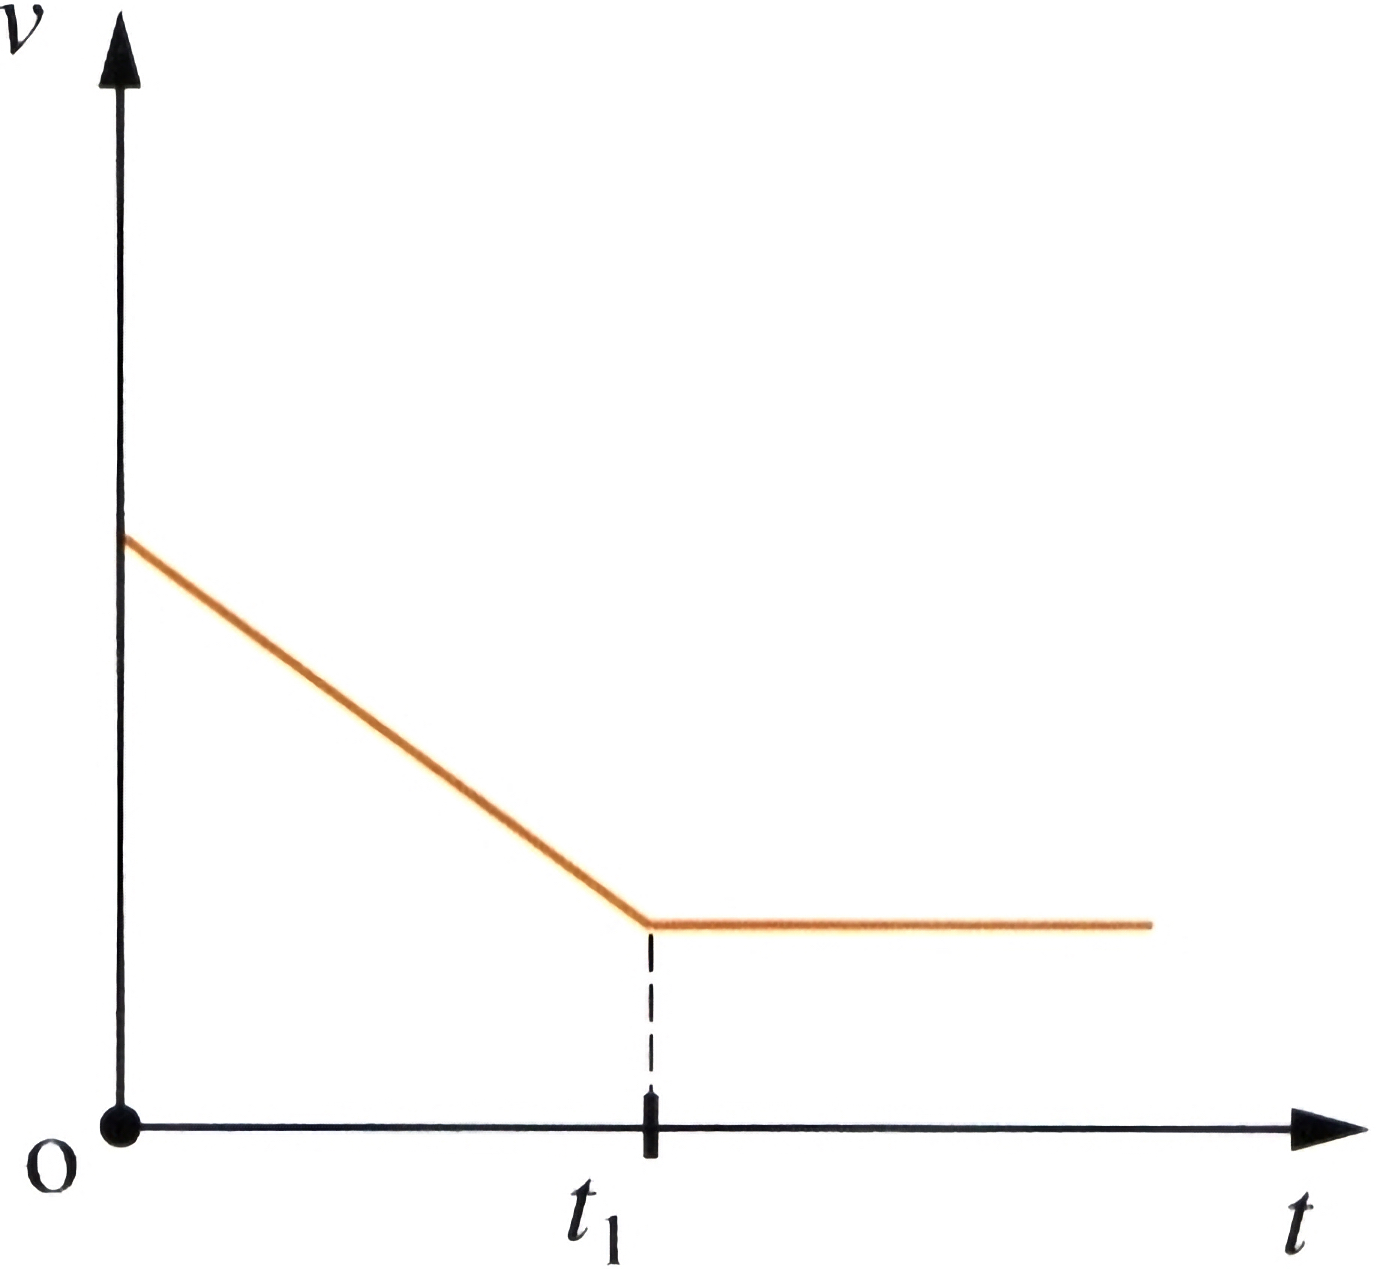
\includegraphics[width=\textwidth]{v(t)}
	\end{image}
\end{exercise}

\begin{exercise}
	De snelheid van een deeltje voldoet aan $v=at$ waarin $a$ constant en negatief is. De plaats van het deeltje wordt voorgesteld door $x$. Aangenomen wordt dat $x=0\rm\,m$ op het ogenblik $t=0\rm\,s$. Welke grafiek geeft het juiste verloop van $x(t)$?
	\begin{multipleChoice}
		\choice{% !TEX root = ../oefeningen_fys6.tex
\begin{tikzpicture}[line cap=round,line join=round,>=triangle 45,x=1.0cm,y=1.0cm, scale=0.8]
\draw[->,color=black] (-0.26126256871071957,0.) -- (3.6896534027248262,0.);
\foreach \x in {,0.5,1.,1.5,2.,2.5,3.,3.5}
\draw[shift={(\x,0)},color=black] (0pt,-2pt);
\draw[->,color=black] (0.,-0.2694355115461891) -- (0.,3.9273529130473617);
\foreach \y in {,0.5,1.,1.5,2.,2.5,3.,3.5}
%\draw[shift={(0,\y)},color=black] (2pt,0pt) -- (-2pt,0pt);
\clip(-0.26126256871071957,-0.2694355115461891) rectangle (3.6896534027248262,3.9273529130473617);
\draw[line width=1.1pt] (0.006830113675660519,2.0136135768984986) -- (0.013660227351321039,2.0271338528913523);
\draw[line width=1.1pt] (0.013660227351321039,2.0271338528913523) -- (0.020490341026981558,2.0405608279785614);
\draw[line width=1.1pt] (0.020490341026981558,2.0405608279785614) -- (0.027320454702642077,2.0538945021601247);
\draw[line width=1.1pt] (0.027320454702642077,2.0538945021601247) -- (0.0341505683783026,2.067134875436044);
\draw[line width=1.1pt] (0.0341505683783026,2.067134875436044) -- (0.040980682053963116,2.080281947806318);
\draw[line width=1.1pt] (0.040980682053963116,2.080281947806318) -- (0.047810795729623635,2.0933357192709474);
\draw[line width=1.1pt] (0.047810795729623635,2.0933357192709474) -- (0.054640909405284155,2.106296189829932);
\draw[line width=1.1pt] (0.054640909405284155,2.106296189829932) -- (0.061471023080944674,2.1191633594832715);
\draw[line width=1.1pt] (0.061471023080944674,2.1191633594832715) -- (0.0683011367566052,2.131937228230966);
\draw[line width=1.1pt] (0.0683011367566052,2.131937228230966) -- (0.0751312504322657,2.1446177960730153);
\draw[line width=1.1pt] (0.0751312504322657,2.1446177960730153) -- (0.08196136410792623,2.15720506300942);
\draw[line width=1.1pt] (0.08196136410792623,2.15720506300942) -- (0.08879147778358676,2.1696990290401805);
\draw[line width=1.1pt] (0.08879147778358676,2.1696990290401805) -- (0.09562159145924728,2.1820996941652955);
\draw[line width=1.1pt] (0.09562159145924728,2.1820996941652955) -- (0.10245170513490781,2.1944070583847655);
\draw[line width=1.1pt] (0.10245170513490781,2.1944070583847655) -- (0.10928181881056834,2.206621121698591);
\draw[line width=1.1pt] (0.10928181881056834,2.206621121698591) -- (0.11611193248622886,2.218741884106771);
\draw[line width=1.1pt] (0.11611193248622886,2.218741884106771) -- (0.12294204616188939,2.2307693456093065);
\draw[line width=1.1pt] (0.12294204616188939,2.2307693456093065) -- (0.12977215983754992,2.242703506206197);
\draw[line width=1.1pt] (0.12977215983754992,2.242703506206197) -- (0.13660227351321044,2.2545443658974427);
\draw[line width=1.1pt] (0.13660227351321044,2.2545443658974427) -- (0.14343238718887097,2.2662919246830437);
\draw[line width=1.1pt] (0.14343238718887097,2.2662919246830437) -- (0.1502625008645315,2.277946182563);
\draw[line width=1.1pt] (0.1502625008645315,2.277946182563) -- (0.15709261454019202,2.289507139537311);
\draw[line width=1.1pt] (0.15709261454019202,2.289507139537311) -- (0.16392272821585255,2.300974795605977);
\draw[line width=1.1pt] (0.16392272821585255,2.300974795605977) -- (0.17075284189151307,2.3123491507689984);
\draw[line width=1.1pt] (0.17075284189151307,2.3123491507689984) -- (0.1775829555671736,2.323630205026374);
\draw[line width=1.1pt] (0.1775829555671736,2.323630205026374) -- (0.18441306924283413,2.334817958378106);
\draw[line width=1.1pt] (0.18441306924283413,2.334817958378106) -- (0.19124318291849465,2.3459124108241927);
\draw[line width=1.1pt] (0.19124318291849465,2.3459124108241927) -- (0.19807329659415518,2.356913562364634);
\draw[line width=1.1pt] (0.19807329659415518,2.356913562364634) -- (0.2049034102698157,2.3678214129994313);
\draw[line width=1.1pt] (0.2049034102698157,2.3678214129994313) -- (0.21173352394547623,2.378635962728583);
\draw[line width=1.1pt] (0.21173352394547623,2.378635962728583) -- (0.21856363762113676,2.38935721155209);
\draw[line width=1.1pt] (0.21856363762113676,2.38935721155209) -- (0.22539375129679728,2.399985159469952);
\draw[line width=1.1pt] (0.22539375129679728,2.399985159469952) -- (0.2322238649724578,2.4105198064821693);
\draw[line width=1.1pt] (0.2322238649724578,2.4105198064821693) -- (0.23905397864811834,2.4209611525887413);
\draw[line width=1.1pt] (0.23905397864811834,2.4209611525887413) -- (0.24588409232377886,2.4313091977896693);
\draw[line width=1.1pt] (0.24588409232377886,2.4313091977896693) -- (0.2527142059994394,2.4415639420849518);
\draw[line width=1.1pt] (0.2527142059994394,2.4415639420849518) -- (0.2595443196750999,2.4517253854745893);
\draw[line width=1.1pt] (0.2595443196750999,2.4517253854745893) -- (0.2663744333507604,2.4617935279585823);
\draw[line width=1.1pt] (0.2663744333507604,2.4617935279585823) -- (0.2732045470264209,2.47176836953693);
\draw[line width=1.1pt] (0.2732045470264209,2.47176836953693) -- (0.2800346607020814,2.481649910209633);
\draw[line width=1.1pt] (0.2800346607020814,2.481649910209633) -- (0.2868647743777419,2.491438149976691);
\draw[line width=1.1pt] (0.2868647743777419,2.491438149976691) -- (0.2936948880534024,2.501133088838104);
\draw[line width=1.1pt] (0.2936948880534024,2.501133088838104) -- (0.3005250017290629,2.5107347267938724);
\draw[line width=1.1pt] (0.3005250017290629,2.5107347267938724) -- (0.3073551154047234,2.520243063843996);
\draw[line width=1.1pt] (0.3073551154047234,2.520243063843996) -- (0.3141852290803839,2.529658099988475);
\draw[line width=1.1pt] (0.3141852290803839,2.529658099988475) -- (0.3210153427560444,2.5389798352273085);
\draw[line width=1.1pt] (0.3210153427560444,2.5389798352273085) -- (0.3278454564317049,2.548208269560497);
\draw[line width=1.1pt] (0.3278454564317049,2.548208269560497) -- (0.33467557010736537,2.5573434029880406);
\draw[line width=1.1pt] (0.33467557010736537,2.5573434029880406) -- (0.34150568378302587,2.56638523550994);
\draw[line width=1.1pt] (0.34150568378302587,2.56638523550994) -- (0.34833579745868637,2.5753337671261933);
\draw[line width=1.1pt] (0.34833579745868637,2.5753337671261933) -- (0.35516591113434687,2.5841889978368027);
\draw[line width=1.1pt] (0.35516591113434687,2.5841889978368027) -- (0.36199602481000737,2.592950927641767);
\draw[line width=1.1pt] (0.36199602481000737,2.592950927641767) -- (0.36882613848566786,2.601619556541087);
\draw[line width=1.1pt] (0.36882613848566786,2.601619556541087) -- (0.37565625216132836,2.6101948845347613);
\draw[line width=1.1pt] (0.37565625216132836,2.6101948845347613) -- (0.38248636583698886,2.618676911622791);
\draw[line width=1.1pt] (0.38248636583698886,2.618676911622791) -- (0.38931647951264936,2.6270656378051758);
\draw[line width=1.1pt] (0.38931647951264936,2.6270656378051758) -- (0.39614659318830986,2.6353610630819158);
\draw[line width=1.1pt] (0.39614659318830986,2.6353610630819158) -- (0.40297670686397036,2.6435631874530103);
\draw[line width=1.1pt] (0.40297670686397036,2.6435631874530103) -- (0.40980682053963086,2.6516720109184604);
\draw[line width=1.1pt] (0.40980682053963086,2.6516720109184604) -- (0.41663693421529135,2.659687533478266);
\draw[line width=1.1pt] (0.41663693421529135,2.659687533478266) -- (0.42346704789095185,2.667609755132426);
\draw[line width=1.1pt] (0.42346704789095185,2.667609755132426) -- (0.43029716156661235,2.6754386758809416);
\draw[line width=1.1pt] (0.43029716156661235,2.6754386758809416) -- (0.43712727524227285,2.683174295723812);
\draw[line width=1.1pt] (0.43712727524227285,2.683174295723812) -- (0.44395738891793335,2.6908166146610375);
\draw[line width=1.1pt] (0.44395738891793335,2.6908166146610375) -- (0.45078750259359385,2.698365632692618);
\draw[line width=1.1pt] (0.45078750259359385,2.698365632692618) -- (0.45761761626925435,2.705821349818554);
\draw[line width=1.1pt] (0.45761761626925435,2.705821349818554) -- (0.46444772994491484,2.713183766038845);
\draw[line width=1.1pt] (0.46444772994491484,2.713183766038845) -- (0.47127784362057534,2.7204528813534914);
\draw[line width=1.1pt] (0.47127784362057534,2.7204528813534914) -- (0.47810795729623584,2.7276286957624927);
\draw[line width=1.1pt] (0.47810795729623584,2.7276286957624927) -- (0.48493807097189634,2.734711209265849);
\draw[line width=1.1pt] (0.48493807097189634,2.734711209265849) -- (0.49176818464755684,2.74170042186356);
\draw[line width=1.1pt] (0.49176818464755684,2.74170042186356) -- (0.49859829832321734,2.7485963335556267);
\draw[line width=1.1pt] (0.49859829832321734,2.7485963335556267) -- (0.5054284119988779,2.7553989443420486);
\draw[line width=1.1pt] (0.5054284119988779,2.7553989443420486) -- (0.5122585256745384,2.762108254222825);
\draw[line width=1.1pt] (0.5122585256745384,2.762108254222825) -- (0.519088639350199,2.768724263197957);
\draw[line width=1.1pt] (0.519088639350199,2.768724263197957) -- (0.5259187530258596,2.775246971267444);
\draw[line width=1.1pt] (0.5259187530258596,2.775246971267444) -- (0.5327488667015201,2.7816763784312863);
\draw[line width=1.1pt] (0.5327488667015201,2.7816763784312863) -- (0.5395789803771807,2.7880124846894834);
\draw[line width=1.1pt] (0.5395789803771807,2.7880124846894834) -- (0.5464090940528412,2.794255290042036);
\draw[line width=1.1pt] (0.5464090940528412,2.794255290042036) -- (0.5532392077285018,2.8004047944889434);
\draw[line width=1.1pt] (0.5532392077285018,2.8004047944889434) -- (0.5600693214041623,2.8064609980302055);
\draw[line width=1.1pt] (0.5600693214041623,2.8064609980302055) -- (0.5668994350798229,2.8124239006658236);
\draw[line width=1.1pt] (0.5668994350798229,2.8124239006658236) -- (0.5737295487554834,2.8182935023957962);
\draw[line width=1.1pt] (0.5737295487554834,2.8182935023957962) -- (0.580559662431144,2.824069803220124);
\draw[line width=1.1pt] (0.580559662431144,2.824069803220124) -- (0.5873897761068045,2.829752803138807);
\draw[line width=1.1pt] (0.5873897761068045,2.829752803138807) -- (0.5942198897824651,2.8353425021518452);
\draw[line width=1.1pt] (0.5942198897824651,2.8353425021518452) -- (0.6010500034581256,2.8408389002592385);
\draw[line width=1.1pt] (0.6010500034581256,2.8408389002592385) -- (0.6078801171337862,2.8462419974609867);
\draw[line width=1.1pt] (0.6078801171337862,2.8462419974609867) -- (0.6147102308094468,2.85155179375709);
\draw[line width=1.1pt] (0.6147102308094468,2.85155179375709) -- (0.6215403444851073,2.8567682891475488);
\draw[line width=1.1pt] (0.6215403444851073,2.8567682891475488) -- (0.6283704581607679,2.8618914836323626);
\draw[line width=1.1pt] (0.6283704581607679,2.8618914836323626) -- (0.6352005718364284,2.866921377211531);
\draw[line width=1.1pt] (0.6352005718364284,2.866921377211531) -- (0.642030685512089,2.8718579698850553);
\draw[line width=1.1pt] (0.642030685512089,2.8718579698850553) -- (0.6488607991877495,2.876701261652934);
\draw[line width=1.1pt] (0.6488607991877495,2.876701261652934) -- (0.6556909128634101,2.881451252515168);
\draw[line width=1.1pt] (0.6556909128634101,2.881451252515168) -- (0.6625210265390706,2.8861079424717575);
\draw[line width=1.1pt] (0.6625210265390706,2.8861079424717575) -- (0.6693511402147312,2.8906713315227015);
\draw[line width=1.1pt] (0.6693511402147312,2.8906713315227015) -- (0.6761812538903917,2.895141419668001);
\draw[line width=1.1pt] (0.6761812538903917,2.895141419668001) -- (0.6830113675660523,2.8995182069076555);
\draw[line width=1.1pt] (0.6830113675660523,2.8995182069076555) -- (0.6898414812417129,2.9038016932416655);
\draw[line width=1.1pt] (0.6898414812417129,2.9038016932416655) -- (0.6966715949173734,2.90799187867003);
\draw[line width=1.1pt] (0.6966715949173734,2.90799187867003) -- (0.703501708593034,2.9120887631927497);
\draw[line width=1.1pt] (0.703501708593034,2.9120887631927497) -- (0.7103318222686945,2.9160923468098248);
\draw[line width=1.1pt] (0.7103318222686945,2.9160923468098248) -- (0.7171619359443551,2.920002629521255);
\draw[line width=1.1pt] (0.7171619359443551,2.920002629521255) -- (0.7239920496200156,2.92381961132704);
\draw[line width=1.1pt] (0.7239920496200156,2.92381961132704) -- (0.7308221632956762,2.9275432922271802);
\draw[line width=1.1pt] (0.7308221632956762,2.9275432922271802) -- (0.7376522769713367,2.931173672221676);
\draw[line width=1.1pt] (0.7376522769713367,2.931173672221676) -- (0.7444823906469973,2.934710751310526);
\draw[line width=1.1pt] (0.7444823906469973,2.934710751310526) -- (0.7513125043226578,2.938154529493732);
\draw[line width=1.1pt] (0.7513125043226578,2.938154529493732) -- (0.7581426179983184,2.9415050067712927);
\draw[line width=1.1pt] (0.7581426179983184,2.9415050067712927) -- (0.764972731673979,2.9447621831432085);
\draw[line width=1.1pt] (0.764972731673979,2.9447621831432085) -- (0.7718028453496395,2.9479260586094793);
\draw[line width=1.1pt] (0.7718028453496395,2.9479260586094793) -- (0.7786329590253,2.9509966331701056);
\draw[line width=1.1pt] (0.7786329590253,2.9509966331701056) -- (0.7854630727009606,2.9539739068250865);
\draw[line width=1.1pt] (0.7854630727009606,2.9539739068250865) -- (0.7922931863766212,2.956857879574423);
\draw[line width=1.1pt] (0.7922931863766212,2.956857879574423) -- (0.7991233000522817,2.9596485514181143);
\draw[line width=1.1pt] (0.7991233000522817,2.9596485514181143) -- (0.8059534137279423,2.962345922356161);
\draw[line width=1.1pt] (0.8059534137279423,2.962345922356161) -- (0.8127835274036028,2.9649499923885623);
\draw[line width=1.1pt] (0.8127835274036028,2.9649499923885623) -- (0.8196136410792634,2.9674607615153192);
\draw[line width=1.1pt] (0.8196136410792634,2.9674607615153192) -- (0.8264437547549239,2.9698782297364312);
\draw[line width=1.1pt] (0.8264437547549239,2.9698782297364312) -- (0.8332738684305845,2.972202397051898);
\draw[line width=1.1pt] (0.8332738684305845,2.972202397051898) -- (0.840103982106245,2.97443326346172);
\draw[line width=1.1pt] (0.840103982106245,2.97443326346172) -- (0.8469340957819056,2.9765708289658974);
\draw[line width=1.1pt] (0.8469340957819056,2.9765708289658974) -- (0.8537642094575661,2.9786150935644296);
\draw[line width=1.1pt] (0.8537642094575661,2.9786150935644296) -- (0.8605943231332267,2.9805660572573167);
\draw[line width=1.1pt] (0.8605943231332267,2.9805660572573167) -- (0.8674244368088873,2.9824237200445594);
\draw[line width=1.1pt] (0.8674244368088873,2.9824237200445594) -- (0.8742545504845478,2.984188081926157);
\draw[line width=1.1pt] (0.8742545504845478,2.984188081926157) -- (0.8810846641602084,2.9858591429021093);
\draw[line width=1.1pt] (0.8810846641602084,2.9858591429021093) -- (0.8879147778358689,2.9874369029724175);
\draw[line width=1.1pt] (0.8879147778358689,2.9874369029724175) -- (0.8947448915115295,2.9889213621370803);
\draw[line width=1.1pt] (0.8947448915115295,2.9889213621370803) -- (0.90157500518719,2.990312520396098);
\draw[line width=1.1pt] (0.90157500518719,2.990312520396098) -- (0.9084051188628506,2.9916103777494714);
\draw[line width=1.1pt] (0.9084051188628506,2.9916103777494714) -- (0.9152352325385111,2.9928149341971997);
\draw[line width=1.1pt] (0.9152352325385111,2.9928149341971997) -- (0.9220653462141717,2.993926189739283);
\draw[line width=1.1pt] (0.9220653462141717,2.993926189739283) -- (0.9288954598898322,2.9949441443757214);
\draw[line width=1.1pt] (0.9288954598898322,2.9949441443757214) -- (0.9357255735654928,2.995868798106515);
\draw[line width=1.1pt] (0.9357255735654928,2.995868798106515) -- (0.9425556872411534,2.9967001509316638);
\draw[line width=1.1pt] (0.9425556872411534,2.9967001509316638) -- (0.9493858009168139,2.9974382028511677);
\draw[line width=1.1pt] (0.9493858009168139,2.9974382028511677) -- (0.9562159145924745,2.9980829538650267);
\draw[line width=1.1pt] (0.9562159145924745,2.9980829538650267) -- (0.963046028268135,2.9986344039732407);
\draw[line width=1.1pt] (0.963046028268135,2.9986344039732407) -- (0.9698761419437956,2.9990925531758097);
\draw[line width=1.1pt] (0.9698761419437956,2.9990925531758097) -- (0.9767062556194561,2.9994574014727338);
\draw[line width=1.1pt] (0.9767062556194561,2.9994574014727338) -- (0.9835363692951167,2.9997289488640133);
\draw[line width=1.1pt] (0.9835363692951167,2.9997289488640133) -- (0.9903664829707772,2.999907195349648);
\draw[line width=1.1pt] (0.9903664829707772,2.999907195349648) -- (0.9971965966464378,2.9999921409296375);
\draw[line width=1.1pt] (0.9971965966464378,2.9999921409296375) -- (1.0040267103220983,2.999983785603982);
\draw[line width=1.1pt] (1.0040267103220983,2.999983785603982) -- (1.010856823997759,2.999882129372682);
\draw[line width=1.1pt] (1.010856823997759,2.999882129372682) -- (1.0176869376734194,2.999687172235736);
\draw[line width=1.1pt] (1.0176869376734194,2.999687172235736) -- (1.02451705134908,2.9993989141931463);
\draw[line width=1.1pt] (1.02451705134908,2.9993989141931463) -- (1.0313471650247406,2.999017355244912);
\draw[line width=1.1pt] (1.0313471650247406,2.999017355244912) -- (1.038177278700401,2.998542495391032);
\draw[line width=1.1pt] (1.038177278700401,2.998542495391032) -- (1.0450073923760617,2.9979743346315066);
\draw[line width=1.1pt] (1.0450073923760617,2.9979743346315066) -- (1.0518375060517222,2.9973128729663374);
\draw[line width=1.1pt] (1.0518375060517222,2.9973128729663374) -- (1.0586676197273828,2.9965581103955237);
\draw[line width=1.1pt] (1.0586676197273828,2.9965581103955237) -- (1.0654977334030433,2.995710046919064);
\draw[line width=1.1pt] (1.0654977334030433,2.995710046919064) -- (1.0723278470787039,2.994768682536959);
\draw[line width=1.1pt] (1.0723278470787039,2.994768682536959) -- (1.0791579607543644,2.9937340172492104);
\draw[line width=1.1pt] (1.0791579607543644,2.9937340172492104) -- (1.085988074430025,2.992606051055817);
\draw[line width=1.1pt] (1.085988074430025,2.992606051055817) -- (1.0928181881056855,2.9913847839567778);
\draw[line width=1.1pt] (1.0928181881056855,2.9913847839567778) -- (1.099648301781346,2.9900702159520933);
\draw[line width=1.1pt] (1.099648301781346,2.9900702159520933) -- (1.1064784154570066,2.988662347041765);
\draw[line width=1.1pt] (1.1064784154570066,2.988662347041765) -- (1.1133085291326672,2.9871611772257918);
\draw[line width=1.1pt] (1.1133085291326672,2.9871611772257918) -- (1.1201386428083278,2.985566706504173);
\draw[line width=1.1pt] (1.1201386428083278,2.985566706504173) -- (1.1269687564839883,2.983878934876909);
\draw[line width=1.1pt] (1.1269687564839883,2.983878934876909) -- (1.1337988701596489,2.982097862344001);
\draw[line width=1.1pt] (1.1337988701596489,2.982097862344001) -- (1.1406289838353094,2.9802234889054486);
\draw[line width=1.1pt] (1.1406289838353094,2.9802234889054486) -- (1.14745909751097,2.9782558145612503);
\draw[line width=1.1pt] (1.14745909751097,2.9782558145612503) -- (1.1542892111866305,2.9761948393114066);
\draw[line width=1.1pt] (1.1542892111866305,2.9761948393114066) -- (1.161119324862291,2.9740405631559197);
\draw[line width=1.1pt] (1.161119324862291,2.9740405631559197) -- (1.1679494385379516,2.971792986094787);
\draw[line width=1.1pt] (1.1679494385379516,2.971792986094787) -- (1.1747795522136122,2.969452108128009);
\draw[line width=1.1pt] (1.1747795522136122,2.969452108128009) -- (1.1816096658892727,2.9670179292555865);
\draw[line width=1.1pt] (1.1816096658892727,2.9670179292555865) -- (1.1884397795649333,2.9644904494775193);
\draw[line width=1.1pt] (1.1884397795649333,2.9644904494775193) -- (1.1952698932405939,2.9618696687938075);
\draw[line width=1.1pt] (1.1952698932405939,2.9618696687938075) -- (1.2021000069162544,2.95915558720445);
\draw[line width=1.1pt] (1.2021000069162544,2.95915558720445) -- (1.208930120591915,2.9563482047094474);
\draw[line width=1.1pt] (1.208930120591915,2.9563482047094474) -- (1.2157602342675755,2.953447521308801);
\draw[line width=1.1pt] (1.2157602342675755,2.953447521308801) -- (1.222590347943236,2.9504535370025096);
\draw[line width=1.1pt] (1.222590347943236,2.9504535370025096) -- (1.2294204616188966,2.947366251790572);
\draw[line width=1.1pt] (1.2294204616188966,2.947366251790572) -- (1.2362505752945572,2.9441856656729906);
\draw[line width=1.1pt] (1.2362505752945572,2.9441856656729906) -- (1.2430806889702177,2.940911778649764);
\draw[line width=1.1pt] (1.2430806889702177,2.940911778649764) -- (1.2499108026458783,2.9375445907208935);
\draw[line width=1.1pt] (1.2499108026458783,2.9375445907208935) -- (1.2567409163215388,2.9340841018863766);
\draw[line width=1.1pt] (1.2567409163215388,2.9340841018863766) -- (1.2635710299971994,2.9305303121462147);
\draw[line width=1.1pt] (1.2635710299971994,2.9305303121462147) -- (1.27040114367286,2.9268832215004092);
\draw[line width=1.1pt] (1.27040114367286,2.9268832215004092) -- (1.2772312573485205,2.923142829948959);
\draw[line width=1.1pt] (1.2772312573485205,2.923142829948959) -- (1.284061371024181,2.9193091374918625);
\draw[line width=1.1pt] (1.284061371024181,2.9193091374918625) -- (1.2908914846998416,2.9153821441291212);
\draw[line width=1.1pt] (1.2908914846998416,2.9153821441291212) -- (1.2977215983755022,2.911361849860736);
\draw[line width=1.1pt] (1.2977215983755022,2.911361849860736) -- (1.3045517120511627,2.9072482546867064);
\draw[line width=1.1pt] (1.3045517120511627,2.9072482546867064) -- (1.3113818257268233,2.9030413586070303);
\draw[line width=1.1pt] (1.3113818257268233,2.9030413586070303) -- (1.3182119394024838,2.8987411616217096);
\draw[line width=1.1pt] (1.3182119394024838,2.8987411616217096) -- (1.3250420530781444,2.894347663730745);
\draw[line width=1.1pt] (1.3250420530781444,2.894347663730745) -- (1.331872166753805,2.889860864934135);
\draw[line width=1.1pt] (1.331872166753805,2.889860864934135) -- (1.3387022804294655,2.8852807652318795);
\draw[line width=1.1pt] (1.3387022804294655,2.8852807652318795) -- (1.345532394105126,2.8806073646239794);
\draw[line width=1.1pt] (1.345532394105126,2.8806073646239794) -- (1.3523625077807866,2.875840663110435);
\draw[line width=1.1pt] (1.3523625077807866,2.875840663110435) -- (1.3591926214564471,2.870980660691246);
\draw[line width=1.1pt] (1.3591926214564471,2.870980660691246) -- (1.3660227351321077,2.866027357366411);
\draw[line width=1.1pt] (1.3660227351321077,2.866027357366411) -- (1.3728528488077683,2.860980753135931);
\draw[line width=1.1pt] (1.3728528488077683,2.860980753135931) -- (1.3796829624834288,2.855840847999807);
\draw[line width=1.1pt] (1.3796829624834288,2.855840847999807) -- (1.3865130761590894,2.8506076419580384);
\draw[line width=1.1pt] (1.3865130761590894,2.8506076419580384) -- (1.39334318983475,2.845281135010624);
\draw[line width=1.1pt] (1.39334318983475,2.845281135010624) -- (1.4001733035104105,2.8398613271575646);
\draw[line width=1.1pt] (1.4001733035104105,2.8398613271575646) -- (1.407003417186071,2.834348218398861);
\draw[line width=1.1pt] (1.407003417186071,2.834348218398861) -- (1.4138335308617316,2.8287418087345126);
\draw[line width=1.1pt] (1.4138335308617316,2.8287418087345126) -- (1.4206636445373921,2.823042098164519);
\draw[line width=1.1pt] (1.4206636445373921,2.823042098164519) -- (1.4274937582130527,2.8172490866888795);
\draw[line width=1.1pt] (1.4274937582130527,2.8172490866888795) -- (1.4343238718887132,2.8113627743075966);
\draw[line width=1.1pt] (1.4343238718887132,2.8113627743075966) -- (1.4411539855643738,2.8053831610206688);
\draw[line width=1.1pt] (1.4411539855643738,2.8053831610206688) -- (1.4479840992400344,2.799310246828095);
\draw[line width=1.1pt] (1.4479840992400344,2.799310246828095) -- (1.454814212915695,2.7931440317298764);
\draw[line width=1.1pt] (1.454814212915695,2.7931440317298764) -- (1.4616443265913555,2.786884515726014);
\draw[line width=1.1pt] (1.4616443265913555,2.786884515726014) -- (1.468474440267016,2.7805316988165063);
\draw[line width=1.1pt] (1.468474440267016,2.7805316988165063) -- (1.4753045539426766,2.774085581001353);
\draw[line width=1.1pt] (1.4753045539426766,2.774085581001353) -- (1.4821346676183371,2.767546162280555);
\draw[line width=1.1pt] (1.4821346676183371,2.767546162280555) -- (1.4889647812939977,2.760913442654113);
\draw[line width=1.1pt] (1.4889647812939977,2.760913442654113) -- (1.4957948949696582,2.754187422122026);
\draw[line width=1.1pt] (1.4957948949696582,2.754187422122026) -- (1.5026250086453188,2.747368100684293);
\draw[line width=1.1pt] (1.5026250086453188,2.747368100684293) -- (1.5094551223209793,2.7404554783409156);
\draw[line width=1.1pt] (1.5094551223209793,2.7404554783409156) -- (1.51628523599664,2.733449555091894);
\draw[line width=1.1pt] (1.51628523599664,2.733449555091894) -- (1.5231153496723004,2.7263503309372275);
\draw[line width=1.1pt] (1.5231153496723004,2.7263503309372275) -- (1.529945463347961,2.719157805876915);
\draw[line width=1.1pt] (1.529945463347961,2.719157805876915) -- (1.5367755770236216,2.7118719799109576);
\draw[line width=1.1pt] (1.5367755770236216,2.7118719799109576) -- (1.543605690699282,2.7044928530393566);
\draw[line width=1.1pt] (1.543605690699282,2.7044928530393566) -- (1.5504358043749427,2.69702042526211);
\draw[line width=1.1pt] (1.5504358043749427,2.69702042526211) -- (1.5572659180506032,2.6894546965792183);
\draw[line width=1.1pt] (1.5572659180506032,2.6894546965792183) -- (1.5640960317262638,2.6817956669906815);
\draw[line width=1.1pt] (1.5640960317262638,2.6817956669906815) -- (1.5709261454019243,2.6740433364965006);
\draw[line width=1.1pt] (1.5709261454019243,2.6740433364965006) -- (1.5777562590775849,2.666197705096675);
\draw[line width=1.1pt] (1.5777562590775849,2.666197705096675) -- (1.5845863727532454,2.6582587727912035);
\draw[line width=1.1pt] (1.5845863727532454,2.6582587727912035) -- (1.591416486428906,2.6502265395800872);
\draw[line width=1.1pt] (1.591416486428906,2.6502265395800872) -- (1.5982466001045665,2.642101005463327);
\draw[line width=1.1pt] (1.5982466001045665,2.642101005463327) -- (1.605076713780227,2.6338821704409217);
\draw[line width=1.1pt] (1.605076713780227,2.6338821704409217) -- (1.6119068274558876,2.6255700345128705);
\draw[line width=1.1pt] (1.6119068274558876,2.6255700345128705) -- (1.6187369411315482,2.6171645976791744);
\draw[line width=1.1pt] (1.6187369411315482,2.6171645976791744) -- (1.6255670548072088,2.6086658599398347);
\draw[line width=1.1pt] (1.6255670548072088,2.6086658599398347) -- (1.6323971684828693,2.60007382129485);
\draw[line width=1.1pt] (1.6323971684828693,2.60007382129485) -- (1.6392272821585299,2.5913884817442194);
\draw[line width=1.1pt] (1.6392272821585299,2.5913884817442194) -- (1.6460573958341904,2.582609841287944);
\draw[line width=1.1pt] (1.6460573958341904,2.582609841287944) -- (1.652887509509851,2.5737378999260243);
\draw[line width=1.1pt] (1.652887509509851,2.5737378999260243) -- (1.6597176231855115,2.5647726576584597);
\draw[line width=1.1pt] (1.6597176231855115,2.5647726576584597) -- (1.666547736861172,2.5557141144852498);
\draw[line width=1.1pt] (1.666547736861172,2.5557141144852498) -- (1.6733778505368326,2.546562270406395);
\draw[line width=1.1pt] (1.6733778505368326,2.546562270406395) -- (1.6802079642124932,2.537317125421896);
\draw[line width=1.1pt] (1.6802079642124932,2.537317125421896) -- (1.6870380778881537,2.527978679531752);
\draw[line width=1.1pt] (1.6870380778881537,2.527978679531752) -- (1.6938681915638143,2.518546932735962);
\draw[line width=1.1pt] (1.6938681915638143,2.518546932735962) -- (1.7006983052394749,2.509021885034527);
\draw[line width=1.1pt] (1.7006983052394749,2.509021885034527) -- (1.7075284189151354,2.4994035364274487);
\draw[line width=1.1pt] (1.7075284189151354,2.4994035364274487) -- (1.714358532590796,2.4896918869147253);
\draw[line width=1.1pt] (1.714358532590796,2.4896918869147253) -- (1.7211886462664565,2.479886936496356);
\draw[line width=1.1pt] (1.7211886462664565,2.479886936496356) -- (1.728018759942117,2.469988685172342);
\draw[line width=1.1pt] (1.728018759942117,2.469988685172342) -- (1.7348488736177776,2.4599971329426835);
\draw[line width=1.1pt] (1.7348488736177776,2.4599971329426835) -- (1.7416789872934382,2.4499122798073802);
\draw[line width=1.1pt] (1.7416789872934382,2.4499122798073802) -- (1.7485091009690987,2.4397341257664316);
\draw[line width=1.1pt] (1.7485091009690987,2.4397341257664316) -- (1.7553392146447593,2.429462670819838);
\draw[line width=1.1pt] (1.7553392146447593,2.429462670819838) -- (1.7621693283204198,2.4190979149676);
\draw[line width=1.1pt] (1.7621693283204198,2.4190979149676) -- (1.7689994419960804,2.4086398582097175);
\draw[line width=1.1pt] (1.7689994419960804,2.4086398582097175) -- (1.775829555671741,2.398088500546189);
\draw[line width=1.1pt] (1.775829555671741,2.398088500546189) -- (1.7826596693474015,2.387443841977016);
\draw[line width=1.1pt] (1.7826596693474015,2.387443841977016) -- (1.789489783023062,2.3767058825021983);
\draw[line width=1.1pt] (1.789489783023062,2.3767058825021983) -- (1.7963198966987226,2.365874622121736);
\draw[line width=1.1pt] (1.7963198966987226,2.365874622121736) -- (1.8031500103743832,2.354950060835628);
\draw[line width=1.1pt] (1.8031500103743832,2.354950060835628) -- (1.8099801240500437,2.3439321986438753);
\draw[line width=1.1pt] (1.8099801240500437,2.3439321986438753) -- (1.8168102377257043,2.3328210355464787);
\draw[line width=1.1pt] (1.8168102377257043,2.3328210355464787) -- (1.8236403514013648,2.3216165715434367);
\draw[line width=1.1pt] (1.8236403514013648,2.3216165715434367) -- (1.8304704650770254,2.3103188066347493);
\draw[line width=1.1pt] (1.8304704650770254,2.3103188066347493) -- (1.837300578752686,2.298927740820417);
\draw[line width=1.1pt] (1.837300578752686,2.298927740820417) -- (1.8441306924283465,2.2874433741004405);
\draw[line width=1.1pt] (1.8441306924283465,2.2874433741004405) -- (1.850960806104007,2.275865706474819);
\draw[line width=1.1pt] (1.850960806104007,2.275865706474819) -- (1.8577909197796676,2.264194737943552);
\draw[line width=1.1pt] (1.8577909197796676,2.264194737943552) -- (1.8646210334553281,2.25243046850664);
\draw[line width=1.1pt] (1.8646210334553281,2.25243046850664) -- (1.8714511471309887,2.240572898164084);
\draw[line width=1.1pt] (1.8714511471309887,2.240572898164084) -- (1.8782812608066493,2.228622026915883);
\draw[line width=1.1pt] (1.8782812608066493,2.228622026915883) -- (1.8851113744823098,2.2165778547620363);
\draw[line width=1.1pt] (1.8851113744823098,2.2165778547620363) -- (1.8919414881579704,2.2044403817025446);
\draw[line width=1.1pt] (1.8919414881579704,2.2044403817025446) -- (1.898771601833631,2.1922096077374094);
\draw[line width=1.1pt] (1.898771601833631,2.1922096077374094) -- (1.9056017155092915,2.1798855328666287);
\draw[line width=1.1pt] (1.9056017155092915,2.1798855328666287) -- (1.912431829184952,2.1674681570902026);
\draw[line width=1.1pt] (1.912431829184952,2.1674681570902026) -- (1.9192619428606126,2.1549574804081315);
\draw[line width=1.1pt] (1.9192619428606126,2.1549574804081315) -- (1.9260920565362731,2.1423535028204164);
\draw[line width=1.1pt] (1.9260920565362731,2.1423535028204164) -- (1.9329221702119337,2.1296562243270563);
\draw[line width=1.1pt] (1.9329221702119337,2.1296562243270563) -- (1.9397522838875942,2.1168656449280503);
\draw[line width=1.1pt] (1.9397522838875942,2.1168656449280503) -- (1.9465823975632548,2.1039817646234);
\draw[line width=1.1pt] (1.9465823975632548,2.1039817646234) -- (1.9534125112389154,2.0910045834131052);
\draw[line width=1.1pt] (1.9534125112389154,2.0910045834131052) -- (1.960242624914576,2.0779341012971657);
\draw[line width=1.1pt] (1.960242624914576,2.0779341012971657) -- (1.9670727385902365,2.0647703182755803);
\draw[line width=1.1pt] (1.9670727385902365,2.0647703182755803) -- (1.973902852265897,2.05151323434835);
\draw[line width=1.1pt] (1.973902852265897,2.05151323434835) -- (1.9807329659415576,2.0381628495154755);
\draw[line width=1.1pt] (1.9807329659415576,2.0381628495154755) -- (1.9875630796172181,2.0247191637769566);
\draw[line width=1.1pt] (1.9875630796172181,2.0247191637769566) -- (1.9943931932928787,2.011182177132792);
\draw[line width=1.1pt] (1.9943931932928787,2.011182177132792) -- (2.001223306968539,1.997551889582983);
\draw[line width=1.1pt] (2.001223306968539,1.997551889582983) -- (2.0080534206441993,1.983828301127529);
\draw[line width=1.1pt] (2.0080534206441993,1.983828301127529) -- (2.0148835343198597,1.9700114117664302);
\draw[line width=1.1pt] (2.0148835343198597,1.9700114117664302) -- (2.02171364799552,1.9561012214996865);
\draw[line width=1.1pt] (2.02171364799552,1.9561012214996865) -- (2.0285437616711803,1.9420977303272986);
\draw[line width=1.1pt] (2.0285437616711803,1.9420977303272986) -- (2.0353738753468407,1.9280009382492649);
\draw[line width=1.1pt] (2.0353738753468407,1.9280009382492649) -- (2.042203989022501,1.9138108452655862);
\draw[line width=1.1pt] (2.042203989022501,1.9138108452655862) -- (2.0490341026981613,1.8995274513762634);
\draw[line width=1.1pt] (2.0490341026981613,1.8995274513762634) -- (2.0558642163738217,1.8851507565812957);
\draw[line width=1.1pt] (2.0558642163738217,1.8851507565812957) -- (2.062694330049482,1.870680760880683);
\draw[line width=1.1pt] (2.062694330049482,1.870680760880683) -- (2.0695244437251423,1.8561174642744245);
\draw[line width=1.1pt] (2.0695244437251423,1.8561174642744245) -- (2.0763545574008027,1.8414608667625219);
\draw[line width=1.1pt] (2.0763545574008027,1.8414608667625219) -- (2.083184671076463,1.8267109683449743);
\draw[line width=1.1pt] (2.083184671076463,1.8267109683449743) -- (2.0900147847521233,1.8118677690217826);
\draw[line width=1.1pt] (2.0900147847521233,1.8118677690217826) -- (2.0968448984277837,1.796931268792945);
\draw[line width=1.1pt] (2.0968448984277837,1.796931268792945) -- (2.103675012103444,1.7819014676584626);
\draw[line width=1.1pt] (2.103675012103444,1.7819014676584626) -- (2.1105051257791043,1.766778365618336);
\draw[line width=1.1pt] (2.1105051257791043,1.766778365618336) -- (2.1173352394547647,1.7515619626725636);
\draw[line width=1.1pt] (2.1173352394547647,1.7515619626725636) -- (2.124165353130425,1.736252258821147);
\draw[line width=1.1pt] (2.124165353130425,1.736252258821147) -- (2.1309954668060853,1.7208492540640847);
\draw[line width=1.1pt] (2.1309954668060853,1.7208492540640847) -- (2.1378255804817456,1.7053529484013783);
\draw[line width=1.1pt] (2.1378255804817456,1.7053529484013783) -- (2.144655694157406,1.689763341833027);
\draw[line width=1.1pt] (2.144655694157406,1.689763341833027) -- (2.1514858078330663,1.6740804343590305);
\draw[line width=1.1pt] (2.1514858078330663,1.6740804343590305) -- (2.1583159215087266,1.6583042259793892);
\draw[line width=1.1pt] (2.1583159215087266,1.6583042259793892) -- (2.165146035184387,1.642434716694103);
\draw[line width=1.1pt] (2.165146035184387,1.642434716694103) -- (2.1719761488600473,1.6264719065031725);
\draw[line width=1.1pt] (2.1719761488600473,1.6264719065031725) -- (2.1788062625357076,1.6104157954065963);
\draw[line width=1.1pt] (2.1788062625357076,1.6104157954065963) -- (2.185636376211368,1.594266383404375);
\draw[line width=1.1pt] (2.185636376211368,1.594266383404375) -- (2.1924664898870283,1.5780236704965098);
\draw[line width=1.1pt] (2.1924664898870283,1.5780236704965098) -- (2.1992966035626886,1.5616876566829996);
\draw[line width=1.1pt] (2.1992966035626886,1.5616876566829996) -- (2.206126717238349,1.5452583419638435);
\draw[line width=1.1pt] (2.206126717238349,1.5452583419638435) -- (2.2129568309140093,1.5287357263390433);
\draw[line width=1.1pt] (2.2129568309140093,1.5287357263390433) -- (2.2197869445896696,1.5121198098085982);
\draw[line width=1.1pt] (2.2197869445896696,1.5121198098085982) -- (2.22661705826533,1.495410592372508);
\draw[line width=1.1pt] (2.22661705826533,1.495410592372508) -- (2.2334471719409903,1.478608074030773);
\draw[line width=1.1pt] (2.2334471719409903,1.478608074030773) -- (2.2402772856166506,1.461712254783393);
\draw[line width=1.1pt] (2.2402772856166506,1.461712254783393) -- (2.247107399292311,1.4447231346303688);
\draw[line width=1.1pt] (2.247107399292311,1.4447231346303688) -- (2.2539375129679713,1.4276407135716989);
\draw[line width=1.1pt] (2.2539375129679713,1.4276407135716989) -- (2.2607676266436316,1.410464991607384);
\draw[line width=1.1pt] (2.2607676266436316,1.410464991607384) -- (2.267597740319292,1.393195968737425);
\draw[line width=1.1pt] (2.267597740319292,1.393195968737425) -- (2.2744278539949523,1.375833644961821);
\draw[line width=1.1pt] (2.2744278539949523,1.375833644961821) -- (2.2812579676706126,1.358378020280571);
\draw[line width=1.1pt] (2.2812579676706126,1.358378020280571) -- (2.288088081346273,1.3408290946936772);
\draw[line width=1.1pt] (2.288088081346273,1.3408290946936772) -- (2.2949181950219333,1.3231868682011383);
\draw[line width=1.1pt] (2.2949181950219333,1.3231868682011383) -- (2.3017483086975936,1.3054513408029544);
\draw[line width=1.1pt] (2.3017483086975936,1.3054513408029544) -- (2.308578422373254,1.2876225124991256);
\draw[line width=1.1pt] (2.308578422373254,1.2876225124991256) -- (2.3154085360489143,1.2697003832896518);
\draw[line width=1.1pt] (2.3154085360489143,1.2697003832896518) -- (2.3222386497245746,1.251684953174534);
\draw[line width=1.1pt] (2.3222386497245746,1.251684953174534) -- (2.329068763400235,1.2335762221537703);
\draw[line width=1.1pt] (2.329068763400235,1.2335762221537703) -- (2.3358988770758953,1.2153741902273625);
\draw[line width=1.1pt] (2.3358988770758953,1.2153741902273625) -- (2.3427289907515556,1.1970788573953088);
\draw[line width=1.1pt] (2.3427289907515556,1.1970788573953088) -- (2.349559104427216,1.1786902236576111);
\draw[line width=1.1pt] (2.349559104427216,1.1786902236576111) -- (2.3563892181028763,1.1602082890142675);
\draw[line width=1.1pt] (2.3563892181028763,1.1602082890142675) -- (2.3632193317785366,1.1416330534652799);
\draw[line width=1.1pt] (2.3632193317785366,1.1416330534652799) -- (2.370049445454197,1.1229645170106473);
\draw[line width=1.1pt] (2.370049445454197,1.1229645170106473) -- (2.3768795591298573,1.1042026796503697);
\draw[line width=1.1pt] (2.3768795591298573,1.1042026796503697) -- (2.3837096728055176,1.0853475413844471);
\draw[line width=1.1pt] (2.3837096728055176,1.0853475413844471) -- (2.390539786481178,1.0663991022128805);
\draw[line width=1.1pt] (2.390539786481178,1.0663991022128805) -- (2.3973699001568383,1.047357362135668);
\draw[line width=1.1pt] (2.3973699001568383,1.047357362135668) -- (2.4042000138324986,1.0282223211528105);
\draw[line width=1.1pt] (2.4042000138324986,1.0282223211528105) -- (2.411030127508159,1.008993979264309);
\draw[line width=1.1pt] (2.411030127508159,1.008993979264309) -- (2.4178602411838193,0.9896723364701616);
\draw[line width=1.1pt] (2.4178602411838193,0.9896723364701616) -- (2.4246903548594796,0.9702573927703702);
\draw[line width=1.1pt] (2.4246903548594796,0.9702573927703702) -- (2.43152046853514,0.9507491481649337);
\draw[line width=1.1pt] (2.43152046853514,0.9507491481649337) -- (2.4383505822108003,0.9311476026538523);
\draw[line width=1.1pt] (2.4383505822108003,0.9311476026538523) -- (2.4451806958864606,0.911452756237126);
\draw[line width=1.1pt] (2.4451806958864606,0.911452756237126) -- (2.452010809562121,0.8916646089147546);
\draw[line width=1.1pt] (2.452010809562121,0.8916646089147546) -- (2.4588409232377813,0.8717831606867383);
\draw[line width=1.1pt] (2.4588409232377813,0.8717831606867383) -- (2.4656710369134416,0.8518084115530771);
\draw[line width=1.1pt] (2.4656710369134416,0.8518084115530771) -- (2.472501150589102,0.8317403615137708);
\draw[line width=1.1pt] (2.472501150589102,0.8317403615137708) -- (2.4793312642647622,0.8115790105688205);
\draw[line width=1.1pt] (2.4793312642647622,0.8115790105688205) -- (2.4861613779404226,0.7913243587182244);
\draw[line width=1.1pt] (2.4861613779404226,0.7913243587182244) -- (2.492991491616083,0.7709764059619841);
\draw[line width=1.1pt] (2.492991491616083,0.7709764059619841) -- (2.4998216052917432,0.750535152300098);
\draw[line width=1.1pt] (2.4998216052917432,0.750535152300098) -- (2.5066517189674036,0.7300005977325679);
\draw[line width=1.1pt] (2.5066517189674036,0.7300005977325679) -- (2.513481832643064,0.7093727422593927);
\draw[line width=1.1pt] (2.513481832643064,0.7093727422593927) -- (2.5203119463187242,0.6886515858805726);
\draw[line width=1.1pt] (2.5203119463187242,0.6886515858805726) -- (2.5271420599943846,0.6678371285961076);
\draw[line width=1.1pt] (2.5271420599943846,0.6678371285961076) -- (2.533972173670045,0.6469293704059975);
\draw[line width=1.1pt] (2.533972173670045,0.6469293704059975) -- (2.5408022873457052,0.6259283113102425);
\draw[line width=1.1pt] (2.5408022873457052,0.6259283113102425) -- (2.5476324010213656,0.6048339513088434);
\draw[line width=1.1pt] (2.5476324010213656,0.6048339513088434) -- (2.554462514697026,0.5836462904017985);
\draw[line width=1.1pt] (2.554462514697026,0.5836462904017985) -- (2.5612926283726862,0.5623653285891095);
\draw[line width=1.1pt] (2.5612926283726862,0.5623653285891095) -- (2.5681227420483466,0.5409910658707746);
\draw[line width=1.1pt] (2.5681227420483466,0.5409910658707746) -- (2.574952855724007,0.5195235022467957);
\draw[line width=1.1pt] (2.574952855724007,0.5195235022467957) -- (2.5817829693996672,0.49796263771717175);
\draw[line width=1.1pt] (2.5817829693996672,0.49796263771717175) -- (2.5886130830753276,0.476308472281902);
\draw[line width=1.1pt] (2.5886130830753276,0.476308472281902) -- (2.595443196750988,0.45456100594098814);
\draw[line width=1.1pt] (2.595443196750988,0.45456100594098814) -- (2.6022733104266482,0.4327202386944302);
\draw[line width=1.1pt] (2.6022733104266482,0.4327202386944302) -- (2.6091034241023086,0.41078617054222644);
\draw[line width=1.1pt] (2.6091034241023086,0.41078617054222644) -- (2.615933537777969,0.3887588014843777);
\draw[line width=1.1pt] (2.615933537777969,0.3887588014843777) -- (2.622763651453629,0.366638131520884);
\draw[line width=1.1pt] (2.622763651453629,0.366638131520884) -- (2.6295937651292896,0.3444241606517462);
\draw[line width=1.1pt] (2.6295937651292896,0.3444241606517462) -- (2.63642387880495,0.32211688887696255);
\draw[line width=1.1pt] (2.63642387880495,0.32211688887696255) -- (2.64325399248061,0.2997163161965348);
\draw[line width=1.1pt] (2.64325399248061,0.2997163161965348) -- (2.6500841061562705,0.27722244261046125);
\draw[line width=1.1pt] (2.6500841061562705,0.27722244261046125) -- (2.656914219831931,0.2546352681187436);
\draw[line width=1.1pt] (2.656914219831931,0.2546352681187436) -- (2.663744333507591,0.23195479272138098);
\draw[line width=1.1pt] (2.663744333507591,0.23195479272138098) -- (2.6705744471832515,0.2091810164183734);
\draw[line width=1.1pt] (2.6705744471832515,0.2091810164183734) -- (2.677404560858912,0.18631393920972084);
\draw[line width=1.1pt] (2.677404560858912,0.18631393920972084) -- (2.684234674534572,0.16335356109542332);
\draw[line width=1.1pt] (2.684234674534572,0.16335356109542332) -- (2.6910647882102325,0.14029988207548172);
\draw[line width=1.1pt] (2.6910647882102325,0.14029988207548172) -- (2.697894901885893,0.11715290214989427);
\draw[line width=1.1pt] (2.697894901885893,0.11715290214989427) -- (2.704725015561553,0.09391262131866185);
\draw[line width=1.1pt] (2.704725015561553,0.09391262131866185) -- (2.7115551292372135,0.07057903958178535);
\draw[line width=1.1pt] (2.7115551292372135,0.07057903958178535) -- (2.718385242912874,0.04715215693926389);
\draw[line width=1.1pt] (2.718385242912874,0.04715215693926389) -- (2.725215356588534,0.023631973391096572);
\draw[line width=1.1pt] (2.725215356588534,0.023631973391096572) -- (2.7320454702641945,0.0);
\draw (0.10330693079942738,3.8849611107787396) node[anchor=north west] {$x$};
\draw (3.0537763686955,0.5) node[anchor=north west] {$t$};
\draw (0.02,0.5) node[anchor=north west] {$O$};
\begin{scriptsize}
\draw [fill=black] (0.,0.) circle (1.1pt);
\end{scriptsize}
\end{tikzpicture}}
		\choice{% !TEX root = ../oefeningen_fys6.tex
\begin{tikzpicture}[line cap=round,line join=round,>=triangle 45,x=1.0cm,y=1.0cm, scale=0.8]
\draw[->,color=black] (-0.26126256871071957,0.) -- (3.6896534027248262,0.);
\foreach \x in {,0.5,1.,1.5,2.,2.5,3.,3.5}
\draw[shift={(\x,0)},color=black] (0pt,-2pt);
\draw[->,color=black] (0.,-0.2694355115461891) -- (0.,3.9273529130473617);
%\foreach \y in {,0.5,1.,1.5,2.,2.5,3.,3.5}
%\draw[shift={(0,\y)},color=black] (2pt,0pt) -- (-2pt,0pt);
\clip(-0.26126256871071957,-0.2694355115461891) rectangle (3.6896534027248262,3.9273529130473617);
\draw (0.10330693079942738,3.8849611107787396) node[anchor=north west] {$x$};
\draw (3.0537763686955,0.5105736501964502) node[anchor=north west] {$t$};
%\draw (0.0015666053547352067,0.0) node[anchor=north west] {$O$};
\draw[line width=1.1pt] (0.00922412450019114,0.0028097795864548553) -- (0.01844824900038228,0.005704643645704737);
\draw[line width=1.1pt] (0.01844824900038228,0.005704643645704737) -- (0.027672373500573423,0.008684592177749646);
\draw[line width=1.1pt] (0.027672373500573423,0.008684592177749646) -- (0.03689649800076456,0.01174962518258958);
\draw[line width=1.1pt] (0.03689649800076456,0.01174962518258958) -- (0.0461206225009557,0.01489974266022454);
\draw[line width=1.1pt] (0.0461206225009557,0.01489974266022454) -- (0.05534474700114684,0.018134944610654527);
\draw[line width=1.1pt] (0.05534474700114684,0.018134944610654527) -- (0.06456887150133798,0.021455231033879543);
\draw[line width=1.1pt] (0.06456887150133798,0.021455231033879543) -- (0.07379299600152912,0.024860601929899584);
\draw[line width=1.1pt] (0.07379299600152912,0.024860601929899584) -- (0.08301712050172026,0.02835105729871465);
\draw[line width=1.1pt] (0.08301712050172026,0.02835105729871465) -- (0.0922412450019114,0.03192659714032474);
\draw[line width=1.1pt] (0.0922412450019114,0.03192659714032474) -- (0.10146536950210254,0.03558722145472986);
\draw[line width=1.1pt] (0.10146536950210254,0.03558722145472986) -- (0.11068949400229368,0.039332930241930006);
\draw[line width=1.1pt] (0.11068949400229368,0.039332930241930006) -- (0.11991361850248482,0.04316372350192518);
\draw[line width=1.1pt] (0.11991361850248482,0.04316372350192518) -- (0.12913774300267597,0.047079601234715385);
\draw[line width=1.1pt] (0.12913774300267597,0.047079601234715385) -- (0.1383618675028671,0.05108056344030061);
\draw[line width=1.1pt] (0.1383618675028671,0.05108056344030061) -- (0.14758599200305825,0.05516661011868086);
\draw[line width=1.1pt] (0.14758599200305825,0.05516661011868086) -- (0.15681011650324939,0.05933774126985614);
\draw[line width=1.1pt] (0.15681011650324939,0.05933774126985614) -- (0.16603424100344052,0.06359395689382644);
\draw[line width=1.1pt] (0.16603424100344052,0.06359395689382644) -- (0.17525836550363166,0.06793525699059177);
\draw[line width=1.1pt] (0.17525836550363166,0.06793525699059177) -- (0.1844824900038228,0.07236164156015212);
\draw[line width=1.1pt] (0.1844824900038228,0.07236164156015212) -- (0.19370661450401394,0.07687311060250751);
\draw[line width=1.1pt] (0.19370661450401394,0.07687311060250751) -- (0.20293073900420508,0.08146966411765792);
\draw[line width=1.1pt] (0.20293073900420508,0.08146966411765792) -- (0.21215486350439622,0.08615130210560336);
\draw[line width=1.1pt] (0.21215486350439622,0.08615130210560336) -- (0.22137898800458736,0.09091802456634382);
\draw[line width=1.1pt] (0.22137898800458736,0.09091802456634382) -- (0.2306031125047785,0.0957698314998793);
\draw[line width=1.1pt] (0.2306031125047785,0.0957698314998793) -- (0.23982723700496963,0.10070672290620983);
\draw[line width=1.1pt] (0.23982723700496963,0.10070672290620983) -- (0.24905136150516077,0.10572869878533536);
\draw[line width=1.1pt] (0.24905136150516077,0.10572869878533536) -- (0.25827548600535194,0.11083575913725595);
\draw[line width=1.1pt] (0.25827548600535194,0.11083575913725595) -- (0.2674996105055431,0.11602790396197156);
\draw[line width=1.1pt] (0.2674996105055431,0.11602790396197156) -- (0.2767237350057343,0.1213051332594822);
\draw[line width=1.1pt] (0.2767237350057343,0.1213051332594822) -- (0.28594785950592544,0.12666744702978786);
\draw[line width=1.1pt] (0.28594785950592544,0.12666744702978786) -- (0.2951719840061166,0.13211484527288855);
\draw[line width=1.1pt] (0.2951719840061166,0.13211484527288855) -- (0.30439610850630777,0.13764732798878426);
\draw[line width=1.1pt] (0.30439610850630777,0.13764732798878426) -- (0.31362023300649894,0.143264895177475);
\draw[line width=1.1pt] (0.31362023300649894,0.143264895177475) -- (0.3228443575066901,0.1489675468389608);
\draw[line width=1.1pt] (0.3228443575066901,0.1489675468389608) -- (0.33206848200688127,0.1547552829732416);
\draw[line width=1.1pt] (0.33206848200688127,0.1547552829732416) -- (0.34129260650707244,0.16062810358031743);
\draw[line width=1.1pt] (0.34129260650707244,0.16062810358031743) -- (0.3505167310072636,0.16658600866018827);
\draw[line width=1.1pt] (0.3505167310072636,0.16658600866018827) -- (0.35974085550745477,0.17262899821285416);
\draw[line width=1.1pt] (0.35974085550745477,0.17262899821285416) -- (0.36896498000764594,0.17875707223831505);
\draw[line width=1.1pt] (0.36896498000764594,0.17875707223831505) -- (0.3781891045078371,0.18497023073657098);
\draw[line width=1.1pt] (0.3781891045078371,0.18497023073657098) -- (0.38741322900802827,0.19126847370762196);
\draw[line width=1.1pt] (0.38741322900802827,0.19126847370762196) -- (0.39663735350821944,0.19765180115146794);
\draw[line width=1.1pt] (0.39663735350821944,0.19765180115146794) -- (0.4058614780084106,0.20412021306810896);
\draw[line width=1.1pt] (0.4058614780084106,0.20412021306810896) -- (0.41508560250860177,0.210673709457545);
\draw[line width=1.1pt] (0.41508560250860177,0.210673709457545) -- (0.42430972700879294,0.21731229031977606);
\draw[line width=1.1pt] (0.42430972700879294,0.21731229031977606) -- (0.4335338515089841,0.22403595565480217);
\draw[line width=1.1pt] (0.4335338515089841,0.22403595565480217) -- (0.44275797600917527,0.23084470546262328);
\draw[line width=1.1pt] (0.44275797600917527,0.23084470546262328) -- (0.45198210050936644,0.23773853974323944);
\draw[line width=1.1pt] (0.45198210050936644,0.23773853974323944) -- (0.4612062250095576,0.2447174584966506);
\draw[line width=1.1pt] (0.4612062250095576,0.2447174584966506) -- (0.47043034950974877,0.2517814617228568);
\draw[line width=1.1pt] (0.47043034950974877,0.2517814617228568) -- (0.47965447400993994,0.25893054942185806);
\draw[line width=1.1pt] (0.47965447400993994,0.25893054942185806) -- (0.4888785985101311,0.2661647215936543);
\draw[line width=1.1pt] (0.4888785985101311,0.2661647215936543) -- (0.49810272301032227,0.2734839782382456);
\draw[line width=1.1pt] (0.49810272301032227,0.2734839782382456) -- (0.5073268475105134,0.28088831935563185);
\draw[line width=1.1pt] (0.5073268475105134,0.28088831935563185) -- (0.5165509720107045,0.28837774494581314);
\draw[line width=1.1pt] (0.5165509720107045,0.28837774494581314) -- (0.5257750965108957,0.2959522550087895);
\draw[line width=1.1pt] (0.5257750965108957,0.2959522550087895) -- (0.5349992210110869,0.30361184954456094);
\draw[line width=1.1pt] (0.5349992210110869,0.30361184954456094) -- (0.544223345511278,0.31135652855312734);
\draw[line width=1.1pt] (0.544223345511278,0.31135652855312734) -- (0.5534474700114692,0.3191862920344888);
\draw[line width=1.1pt] (0.5534474700114692,0.3191862920344888) -- (0.5626715945116604,0.32710113998864526);
\draw[line width=1.1pt] (0.5626715945116604,0.32710113998864526) -- (0.5718957190118515,0.3351010724155968);
\draw[line width=1.1pt] (0.5718957190118515,0.3351010724155968) -- (0.5811198435120427,0.34318608931534333);
\draw[line width=1.1pt] (0.5811198435120427,0.34318608931534333) -- (0.5903439680122339,0.3513561906878848);
\draw[line width=1.1pt] (0.5903439680122339,0.3513561906878848) -- (0.599568092512425,0.3596113765332214);
\draw[line width=1.1pt] (0.599568092512425,0.3596113765332214) -- (0.6087922170126162,0.36795164685135306);
\draw[line width=1.1pt] (0.6087922170126162,0.36795164685135306) -- (0.6180163415128074,0.37637700164227966);
\draw[line width=1.1pt] (0.6180163415128074,0.37637700164227966) -- (0.6272404660129985,0.38488744090600135);
\draw[line width=1.1pt] (0.6272404660129985,0.38488744090600135) -- (0.6364645905131897,0.39348296464251803);
\draw[line width=1.1pt] (0.6364645905131897,0.39348296464251803) -- (0.6456887150133809,0.40216357285182974);
\draw[line width=1.1pt] (0.6456887150133809,0.40216357285182974) -- (0.654912839513572,0.4109292655339365);
\draw[line width=1.1pt] (0.654912839513572,0.4109292655339365) -- (0.6641369640137632,0.4197800426888383);
\draw[line width=1.1pt] (0.6641369640137632,0.4197800426888383) -- (0.6733610885139544,0.42871590431653506);
\draw[line width=1.1pt] (0.6733610885139544,0.42871590431653506) -- (0.6825852130141455,0.43773685041702687);
\draw[line width=1.1pt] (0.6825852130141455,0.43773685041702687) -- (0.6918093375143367,0.4468428809903137);
\draw[line width=1.1pt] (0.6918093375143367,0.4468428809903137) -- (0.7010334620145279,0.4560339960363956);
\draw[line width=1.1pt] (0.7010334620145279,0.4560339960363956) -- (0.710257586514719,0.46531019555527253);
\draw[line width=1.1pt] (0.710257586514719,0.46531019555527253) -- (0.7194817110149102,0.47467147954694444);
\draw[line width=1.1pt] (0.7194817110149102,0.47467147954694444) -- (0.7287058355151014,0.48411784801141133);
\draw[line width=1.1pt] (0.7287058355151014,0.48411784801141133) -- (0.7379299600152925,0.4936493009486733);
\draw[line width=1.1pt] (0.7379299600152925,0.4936493009486733) -- (0.7471540845154837,0.5032658383587304);
\draw[line width=1.1pt] (0.7471540845154837,0.5032658383587304) -- (0.7563782090156749,0.5129674602415825);
\draw[line width=1.1pt] (0.7563782090156749,0.5129674602415825) -- (0.765602333515866,0.5227541665972295);
\draw[line width=1.1pt] (0.765602333515866,0.5227541665972295) -- (0.7748264580160572,0.5326259574256715);
\draw[line width=1.1pt] (0.7748264580160572,0.5326259574256715) -- (0.7840505825162484,0.5425828327269087);
\draw[line width=1.1pt] (0.7840505825162484,0.5425828327269087) -- (0.7932747070164395,0.5526247925009409);
\draw[line width=1.1pt] (0.7932747070164395,0.5526247925009409) -- (0.8024988315166307,0.562751836747768);
\draw[line width=1.1pt] (0.8024988315166307,0.562751836747768) -- (0.8117229560168219,0.5729639654673903);
\draw[line width=1.1pt] (0.8117229560168219,0.5729639654673903) -- (0.820947080517013,0.5832611786598074);
\draw[line width=1.1pt] (0.820947080517013,0.5832611786598074) -- (0.8301712050172042,0.5936434763250197);
\draw[line width=1.1pt] (0.8301712050172042,0.5936434763250197) -- (0.8393953295173954,0.604110858463027);
\draw[line width=1.1pt] (0.8393953295173954,0.604110858463027) -- (0.8486194540175865,0.6146633250738294);
\draw[line width=1.1pt] (0.8486194540175865,0.6146633250738294) -- (0.8578435785177777,0.6253008761574266);
\draw[line width=1.1pt] (0.8578435785177777,0.6253008761574266) -- (0.8670677030179689,0.636023511713819);
\draw[line width=1.1pt] (0.8670677030179689,0.636023511713819) -- (0.87629182751816,0.6468312317430064);
\draw[line width=1.1pt] (0.87629182751816,0.6468312317430064) -- (0.8855159520183512,0.6577240362449888);
\draw[line width=1.1pt] (0.8855159520183512,0.6577240362449888) -- (0.8947400765185424,0.6687019252197662);
\draw[line width=1.1pt] (0.8947400765185424,0.6687019252197662) -- (0.9039642010187335,0.6797648986673388);
\draw[line width=1.1pt] (0.9039642010187335,0.6797648986673388) -- (0.9131883255189247,0.6909129565877062);
\draw[line width=1.1pt] (0.9131883255189247,0.6909129565877062) -- (0.9224124500191159,0.7021460989808688);
\draw[line width=1.1pt] (0.9224124500191159,0.7021460989808688) -- (0.931636574519307,0.7134643258468263);
\draw[line width=1.1pt] (0.931636574519307,0.7134643258468263) -- (0.9408606990194982,0.7248676371855789);
\draw[line width=1.1pt] (0.9408606990194982,0.7248676371855789) -- (0.9500848235196894,0.7363560329971265);
\draw[line width=1.1pt] (0.9500848235196894,0.7363560329971265) -- (0.9593089480198805,0.7479295132814692);
\draw[line width=1.1pt] (0.9593089480198805,0.7479295132814692) -- (0.9685330725200717,0.7595880780386068);
\draw[line width=1.1pt] (0.9685330725200717,0.7595880780386068) -- (0.9777571970202629,0.7713317272685394);
\draw[line width=1.1pt] (0.9777571970202629,0.7713317272685394) -- (0.986981321520454,0.7831604609712672);
\draw[line width=1.1pt] (0.986981321520454,0.7831604609712672) -- (0.9962054460206452,0.79507427914679);
\draw[line width=1.1pt] (0.9962054460206452,0.79507427914679) -- (1.0054295705208363,0.8070731817951076);
\draw[line width=1.1pt] (1.0054295705208363,0.8070731817951076) -- (1.0146536950210274,0.8191571689162203);
\draw[line width=1.1pt] (1.0146536950210274,0.8191571689162203) -- (1.0238778195212186,0.831326240510128);
\draw[line width=1.1pt] (1.0238778195212186,0.831326240510128) -- (1.0331019440214098,0.8435803965768309);
\draw[line width=1.1pt] (1.0331019440214098,0.8435803965768309) -- (1.042326068521601,0.8559196371163289);
\draw[line width=1.1pt] (1.042326068521601,0.8559196371163289) -- (1.051550193021792,0.8683439621286217);
\draw[line width=1.1pt] (1.051550193021792,0.8683439621286217) -- (1.0607743175219833,0.8808533716137097);
\draw[line width=1.1pt] (1.0607743175219833,0.8808533716137097) -- (1.0699984420221744,0.8934478655715925);
\draw[line width=1.1pt] (1.0699984420221744,0.8934478655715925) -- (1.0792225665223656,0.9061274440022706);
\draw[line width=1.1pt] (1.0792225665223656,0.9061274440022706) -- (1.0884466910225568,0.9188921069057436);
\draw[line width=1.1pt] (1.0884466910225568,0.9188921069057436) -- (1.097670815522748,0.9317418542820115);
\draw[line width=1.1pt] (1.097670815522748,0.9317418542820115) -- (1.106894940022939,0.9446766861310747);
\draw[line width=1.1pt] (1.106894940022939,0.9446766861310747) -- (1.1161190645231303,0.9576966024529328);
\draw[line width=1.1pt] (1.1161190645231303,0.9576966024529328) -- (1.1253431890233214,0.9708016032475859);
\draw[line width=1.1pt] (1.1253431890233214,0.9708016032475859) -- (1.1345673135235126,0.9839916885150339);
\draw[line width=1.1pt] (1.1345673135235126,0.9839916885150339) -- (1.1437914380237038,0.9972668582552773);
\draw[line width=1.1pt] (1.1437914380237038,0.9972668582552773) -- (1.153015562523895,1.0106271124683155);
\draw[line width=1.1pt] (1.153015562523895,1.0106271124683155) -- (1.162239687024086,1.0240724511541486);
\draw[line width=1.1pt] (1.162239687024086,1.0240724511541486) -- (1.1714638115242773,1.0376028743127768);
\draw[line width=1.1pt] (1.1714638115242773,1.0376028743127768) -- (1.1806879360244684,1.0512183819442);
\draw[line width=1.1pt] (1.1806879360244684,1.0512183819442) -- (1.1899120605246596,1.0649189740484184);
\draw[line width=1.1pt] (1.1899120605246596,1.0649189740484184) -- (1.1991361850248508,1.0787046506254319);
\draw[line width=1.1pt] (1.1991361850248508,1.0787046506254319) -- (1.208360309525042,1.0925754116752402);
\draw[line width=1.1pt] (1.208360309525042,1.0925754116752402) -- (1.217584434025233,1.1065312571978434);
\draw[line width=1.1pt] (1.217584434025233,1.1065312571978434) -- (1.2268085585254243,1.120572187193242);
\draw[line width=1.1pt] (1.2268085585254243,1.120572187193242) -- (1.2360326830256154,1.1346982016614353);
\draw[line width=1.1pt] (1.2360326830256154,1.1346982016614353) -- (1.2452568075258066,1.1489093006024238);
\draw[line width=1.1pt] (1.2452568075258066,1.1489093006024238) -- (1.2544809320259978,1.1632054840162074);
\draw[line width=1.1pt] (1.2544809320259978,1.1632054840162074) -- (1.263705056526189,1.1775867519027858);
\draw[line width=1.1pt] (1.263705056526189,1.1775867519027858) -- (1.27292918102638,1.1920531042621594);
\draw[line width=1.1pt] (1.27292918102638,1.1920531042621594) -- (1.2821533055265713,1.206604541094328);
\draw[line width=1.1pt] (1.2821533055265713,1.206604541094328) -- (1.2913774300267624,1.2212410623992915);
\draw[line width=1.1pt] (1.2913774300267624,1.2212410623992915) -- (1.3006015545269536,1.2359626681770501);
\draw[line width=1.1pt] (1.3006015545269536,1.2359626681770501) -- (1.3098256790271448,1.2507693584276038);
\draw[line width=1.1pt] (1.3098256790271448,1.2507693584276038) -- (1.319049803527336,1.2656611331509524);
\draw[line width=1.1pt] (1.319049803527336,1.2656611331509524) -- (1.328273928027527,1.2806379923470963);
\draw[line width=1.1pt] (1.328273928027527,1.2806379923470963) -- (1.3374980525277183,1.295699936016035);
\draw[line width=1.1pt] (1.3374980525277183,1.295699936016035) -- (1.3467221770279094,1.3108469641577687);
\draw[line width=1.1pt] (1.3467221770279094,1.3108469641577687) -- (1.3559463015281006,1.3260790767722974);
\draw[line width=1.1pt] (1.3559463015281006,1.3260790767722974) -- (1.3651704260282918,1.3413962738596212);
\draw[line width=1.1pt] (1.3651704260282918,1.3413962738596212) -- (1.374394550528483,1.3567985554197401);
\draw[line width=1.1pt] (1.374394550528483,1.3567985554197401) -- (1.383618675028674,1.372285921452654);
\draw[line width=1.1pt] (1.383618675028674,1.372285921452654) -- (1.3928427995288652,1.3878583719583628);
\draw[line width=1.1pt] (1.3928427995288652,1.3878583719583628) -- (1.4020669240290564,1.4035159069368668);
\draw[line width=1.1pt] (1.4020669240290564,1.4035159069368668) -- (1.4112910485292476,1.4192585263881659);
\draw[line width=1.1pt] (1.4112910485292476,1.4192585263881659) -- (1.4205151730294387,1.4350862303122598);
\draw[line width=1.1pt] (1.4205151730294387,1.4350862303122598) -- (1.42973929752963,1.4509990187091488);
\draw[line width=1.1pt] (1.42973929752963,1.4509990187091488) -- (1.438963422029821,1.466996891578833);
\draw[line width=1.1pt] (1.438963422029821,1.466996891578833) -- (1.4481875465300122,1.483079848921312);
\draw[line width=1.1pt] (1.4481875465300122,1.483079848921312) -- (1.4574116710302034,1.499247890736586);
\draw[line width=1.1pt] (1.4574116710302034,1.499247890736586) -- (1.4666357955303946,1.515501017024655);
\draw[line width=1.1pt] (1.4666357955303946,1.515501017024655) -- (1.4758599200305857,1.5318392277855193);
\draw[line width=1.1pt] (1.4758599200305857,1.5318392277855193) -- (1.485084044530777,1.5482625230191784);
\draw[line width=1.1pt] (1.485084044530777,1.5482625230191784) -- (1.494308169030968,1.5647709027256327);
\draw[line width=1.1pt] (1.494308169030968,1.5647709027256327) -- (1.5035322935311592,1.5813643669048818);
\draw[line width=1.1pt] (1.5035322935311592,1.5813643669048818) -- (1.5127564180313504,1.598042915556926);
\draw[line width=1.1pt] (1.5127564180313504,1.598042915556926) -- (1.5219805425315416,1.6148065486817653);
\draw[line width=1.1pt] (1.5219805425315416,1.6148065486817653) -- (1.5312046670317327,1.6316552662793997);
\draw[line width=1.1pt] (1.5312046670317327,1.6316552662793997) -- (1.540428791531924,1.648589068349829);
\draw[line width=1.1pt] (1.540428791531924,1.648589068349829) -- (1.549652916032115,1.6656079548930534);
\draw[line width=1.1pt] (1.549652916032115,1.6656079548930534) -- (1.5588770405323062,1.6827119259090728);
\draw[line width=1.1pt] (1.5588770405323062,1.6827119259090728) -- (1.5681011650324974,1.6999009813978871);
\draw[line width=1.1pt] (1.5681011650324974,1.6999009813978871) -- (1.5773252895326886,1.7171751213594966);
\draw[line width=1.1pt] (1.5773252895326886,1.7171751213594966) -- (1.5865494140328797,1.734534345793901);
\draw[line width=1.1pt] (1.5865494140328797,1.734534345793901) -- (1.595773538533071,1.7519786547011005);
\draw[line width=1.1pt] (1.595773538533071,1.7519786547011005) -- (1.604997663033262,1.769508048081095);
\draw[line width=1.1pt] (1.604997663033262,1.769508048081095) -- (1.6142217875334532,1.7871225259338845);
\draw[line width=1.1pt] (1.6142217875334532,1.7871225259338845) -- (1.6234459120336444,1.8048220882594692);
\draw[line width=1.1pt] (1.6234459120336444,1.8048220882594692) -- (1.6326700365338356,1.8226067350578488);
\draw[line width=1.1pt] (1.6326700365338356,1.8226067350578488) -- (1.6418941610340267,1.8404764663290234);
\draw[line width=1.1pt] (1.6418941610340267,1.8404764663290234) -- (1.651118285534218,1.858431282072993);
\draw[line width=1.1pt] (1.651118285534218,1.858431282072993) -- (1.660342410034409,1.8764711822897577);
\draw[line width=1.1pt] (1.660342410034409,1.8764711822897577) -- (1.6695665345346002,1.8945961669793174);
\draw[line width=1.1pt] (1.6695665345346002,1.8945961669793174) -- (1.6787906590347914,1.9128062361416718);
\draw[line width=1.1pt] (1.6787906590347914,1.9128062361416718) -- (1.6880147835349826,1.9311013897768219);
\draw[line width=1.1pt] (1.6880147835349826,1.9311013897768219) -- (1.6972389080351737,1.9494816278847664);
\draw[line width=1.1pt] (1.6972389080351737,1.9494816278847664) -- (1.706463032535365,1.9679469504655063);
\draw[line width=1.1pt] (1.706463032535365,1.9679469504655063) -- (1.715687157035556,1.986497357519041);
\draw[line width=1.1pt] (1.715687157035556,1.986497357519041) -- (1.7249112815357472,2.005132849045371);
\draw[line width=1.1pt] (1.7249112815357472,2.005132849045371) -- (1.7341354060359384,2.023853425044496);
\draw[line width=1.1pt] (1.7341354060359384,2.023853425044496) -- (1.7433595305361296,2.0426590855164157);
\draw[line width=1.1pt] (1.7433595305361296,2.0426590855164157) -- (1.7525836550363207,2.061549830461131);
\draw[line width=1.1pt] (1.7525836550363207,2.061549830461131) -- (1.761807779536512,2.080525659878641);
\draw[line width=1.1pt] (1.761807779536512,2.080525659878641) -- (1.771031904036703,2.0995865737689456);
\draw[line width=1.1pt] (1.771031904036703,2.0995865737689456) -- (1.7802560285368942,2.118732572132046);
\draw[line width=1.1pt] (1.7802560285368942,2.118732572132046) -- (1.7894801530370854,2.137963654967941);
\draw[line width=1.1pt] (1.7894801530370854,2.137963654967941) -- (1.7987042775372766,2.1572798222766307);
\draw[line width=1.1pt] (1.7987042775372766,2.1572798222766307) -- (1.8079284020374677,2.176681074058116);
\draw[line width=1.1pt] (1.8079284020374677,2.176681074058116) -- (1.817152526537659,2.196167410312396);
\draw[line width=1.1pt] (1.817152526537659,2.196167410312396) -- (1.82637665103785,2.2157388310394714);
\draw[line width=1.1pt] (1.82637665103785,2.2157388310394714) -- (1.8356007755380412,2.2353953362393417);
\draw[line width=1.1pt] (1.8356007755380412,2.2353953362393417) -- (1.8448249000382324,2.255136925912007);
\draw[line width=1.1pt] (1.8448249000382324,2.255136925912007) -- (1.8540490245384236,2.274963600057467);
\draw[line width=1.1pt] (1.8540490245384236,2.274963600057467) -- (1.8632731490386147,2.2948753586757222);
\draw[line width=1.1pt] (1.8632731490386147,2.2948753586757222) -- (1.872497273538806,2.3148722017667724);
\draw[line width=1.1pt] (1.872497273538806,2.3148722017667724) -- (1.881721398038997,2.334954129330618);
\draw[line width=1.1pt] (1.881721398038997,2.334954129330618) -- (1.8909455225391882,2.3551211413672584);
\draw[line width=1.1pt] (1.8909455225391882,2.3551211413672584) -- (1.9001696470393794,2.3753732378766936);
\draw[line width=1.1pt] (1.9001696470393794,2.3753732378766936) -- (1.9093937715395706,2.395710418858924);
\draw[line width=1.1pt] (1.9093937715395706,2.395710418858924) -- (1.9186178960397617,2.4161326843139492);
\draw[line width=1.1pt] (1.9186178960397617,2.4161326843139492) -- (1.927842020539953,2.43664003424177);
\draw[line width=1.1pt] (1.927842020539953,2.43664003424177) -- (1.937066145040144,2.457232468642385);
\draw[line width=1.1pt] (1.937066145040144,2.457232468642385) -- (1.9462902695403352,2.4779099875157957);
\draw[line width=1.1pt] (1.9462902695403352,2.4779099875157957) -- (1.9555143940405264,2.4986725908620016);
\draw[line width=1.1pt] (1.9555143940405264,2.4986725908620016) -- (1.9647385185407176,2.519520278681002);
\draw[line width=1.1pt] (1.9647385185407176,2.519520278681002) -- (1.9739626430409087,2.5404530509727974);
\draw[line width=1.1pt] (1.9739626430409087,2.5404530509727974) -- (1.9831867675411,2.5614709077373883);
\draw[line width=1.1pt] (1.9831867675411,2.5614709077373883) -- (1.992410892041291,2.582573848974774);
\draw[line width=1.1pt] (1.992410892041291,2.582573848974774) -- (2.0016350165414822,2.6037618746849542);
\draw[line width=1.1pt] (2.0016350165414822,2.6037618746849542) -- (2.0108591410416734,2.62503498486793);
\draw[line width=1.1pt] (2.0108591410416734,2.62503498486793) -- (2.0200832655418646,2.646393179523701);
\draw[line width=1.1pt] (2.0200832655418646,2.646393179523701) -- (2.0293073900420557,2.6678364586522667);
\draw[line width=1.1pt] (2.0293073900420557,2.6678364586522667) -- (2.038531514542247,2.6893648222536273);
\draw[line width=1.1pt] (2.038531514542247,2.6893648222536273) -- (2.047755639042438,2.710978270327783);
\draw[line width=1.1pt] (2.047755639042438,2.710978270327783) -- (2.0569797635426292,2.732676802874734);
\draw[line width=1.1pt] (2.0569797635426292,2.732676802874734) -- (2.0662038880428204,2.75446041989448);
\draw[line width=1.1pt] (2.0662038880428204,2.75446041989448) -- (2.0754280125430116,2.776329121387021);
\draw[line width=1.1pt] (2.0754280125430116,2.776329121387021) -- (2.0846521370432027,2.7982829073523567);
\draw[line width=1.1pt] (2.0846521370432027,2.7982829073523567) -- (2.093876261543394,2.8203217777904874);
\draw[line width=1.1pt] (2.093876261543394,2.8203217777904874) -- (2.103100386043585,2.8424457327014134);
\draw[line width=1.1pt] (2.103100386043585,2.8424457327014134) -- (2.1123245105437762,2.8646547720851347);
\draw[line width=1.1pt] (2.1123245105437762,2.8646547720851347) -- (2.1215486350439674,2.8869488959416505);
\draw[line width=1.1pt] (2.1215486350439674,2.8869488959416505) -- (2.1307727595441586,2.9093281042709616);
\draw[line width=1.1pt] (2.1307727595441586,2.9093281042709616) -- (2.1399968840443497,2.931792397073068);
\draw[line width=1.1pt] (2.1399968840443497,2.931792397073068) -- (2.149221008544541,2.9543417743479687);
\draw[line width=1.1pt] (2.149221008544541,2.9543417743479687) -- (2.158445133044732,2.976976236095665);
\draw[line width=1.1pt] (2.158445133044732,2.976976236095665) -- (2.1676692575449232,2.9996957823161563);
\draw[line width=1.1pt] (2.1676692575449232,2.9996957823161563) -- (2.1768933820451144,3.022500413009442);
\draw[line width=1.1pt] (2.1768933820451144,3.022500413009442) -- (2.1861175065453056,3.0453901281755233);
\draw[line width=1.1pt] (2.1861175065453056,3.0453901281755233) -- (2.1953416310454967,3.0683649278144);
\draw[line width=1.1pt] (2.1953416310454967,3.0683649278144) -- (2.204565755545688,3.091424811926071);
\draw[line width=1.1pt] (2.204565755545688,3.091424811926071) -- (2.213789880045879,3.1145697805105375);
\draw[line width=1.1pt] (2.213789880045879,3.1145697805105375) -- (2.2230140045460702,3.1377998335677986);
\draw[line width=1.1pt] (2.2230140045460702,3.1377998335677986) -- (2.2322381290462614,3.161114971097855);
\draw[line width=1.1pt] (2.2322381290462614,3.161114971097855) -- (2.2414622535464526,3.1845151931007063);
\draw[line width=1.1pt] (2.2414622535464526,3.1845151931007063) -- (2.2506863780466437,3.208000499576353);
\draw[line width=1.1pt] (2.2506863780466437,3.208000499576353) -- (2.259910502546835,3.2315708905247944);
\draw[line width=1.1pt] (2.259910502546835,3.2315708905247944) -- (2.269134627047026,3.2552263659460308);
\draw[line width=1.1pt] (2.269134627047026,3.2552263659460308) -- (2.2783587515472172,3.278966925840062);
\draw[line width=1.1pt] (2.2783587515472172,3.278966925840062) -- (2.2875828760474084,3.3027925702068885);
\draw[line width=1.1pt] (2.2875828760474084,3.3027925702068885) -- (2.2968070005475996,3.3267032990465104);
\draw[line width=1.1pt] (2.2968070005475996,3.3267032990465104) -- (2.3060311250477907,3.3506991123589267);
\draw[line width=1.1pt] (2.3060311250477907,3.3506991123589267) -- (2.315255249547982,3.3747800101441383);
\draw[line width=1.1pt] (2.315255249547982,3.3747800101441383) -- (2.324479374048173,3.398945992402145);
\draw[line width=1.1pt] (2.324479374048173,3.398945992402145) -- (2.3337034985483642,3.4231970591329466);
\draw[line width=1.1pt] (2.3337034985483642,3.4231970591329466) -- (2.3429276230485554,3.4475332103365433);
\draw[line width=1.1pt] (2.3429276230485554,3.4475332103365433) -- (2.3521517475487466,3.471954446012935);
\draw[line width=1.1pt] (2.3521517475487466,3.471954446012935) -- (2.3613758720489377,3.4964607661621216);
\draw[line width=1.1pt] (2.3613758720489377,3.4964607661621216) -- (2.370599996549129,3.5210521707841034);
\draw[line width=1.1pt] (2.370599996549129,3.5210521707841034) -- (2.37982412104932,3.5457286598788804);
\draw[line width=1.1pt] (2.37982412104932,3.5457286598788804) -- (2.3890482455495112,3.570490233446452);
\draw[line width=1.1pt] (2.3890482455495112,3.570490233446452) -- (2.3982723700497024,3.5953368914868187);
\draw[line width=1.1pt] (2.3982723700497024,3.5953368914868187) -- (2.4074964945498936,3.620268633999981);
\draw[line width=1.1pt] (2.4074964945498936,3.620268633999981) -- (2.4167206190500847,3.6452854609859378);
\draw[line width=1.1pt] (2.4167206190500847,3.6452854609859378) -- (2.425944743550276,3.6703873724446896);
\draw[line width=1.1pt] (2.425944743550276,3.6703873724446896) -- (2.435168868050467,3.6955743683762363);
\draw[line width=1.1pt] (2.435168868050467,3.6955743683762363) -- (2.4443929925506582,3.7208464487805784);
\draw[line width=1.1pt] (2.4443929925506582,3.7208464487805784) -- (2.4536171170508494,3.7462036136577153);
\draw[line width=1.1pt] (2.4536171170508494,3.7462036136577153) -- (2.4628412415510406,3.7716458630076475);
\draw[line width=1.1pt] (2.4628412415510406,3.7716458630076475) -- (2.4720653660512317,3.7971731968303746);
\draw[line width=1.1pt] (2.4720653660512317,3.7971731968303746) -- (2.481289490551423,3.8227856151258965);
\draw[line width=1.1pt] (2.481289490551423,3.8227856151258965) -- (2.490513615051614,3.848483117894214);
\draw[line width=1.1pt] (2.490513615051614,3.848483117894214) -- (2.4997377395518052,3.874265705135326);
\draw[line width=1.1pt] (2.4997377395518052,3.874265705135326) -- (2.5089618640519964,3.900133376849233);
\draw[line width=1.1pt] (2.5089618640519964,3.900133376849233) -- (2.5181859885521876,3.9260861330359353);
\draw[line width=1.1pt] (2.5181859885521876,3.9260861330359353) -- (2.5274101130523787,3.9521239736954326);
\draw[line width=1.1pt] (2.5274101130523787,3.9521239736954326) -- (2.53663423755257,3.9782468988277246);
\draw[line width=1.1pt] (2.53663423755257,3.9782468988277246) -- (2.545858362052761,4.0044549084328125);
\draw[line width=1.1pt] (2.545858362052761,4.0044549084328125) -- (2.5550824865529522,4.030748002510695);
\draw[line width=1.1pt] (2.5550824865529522,4.030748002510695) -- (2.5643066110531434,4.0571261810613715);
\draw[line width=1.1pt] (2.5643066110531434,4.0571261810613715) -- (2.5735307355533346,4.083589444084844);
\draw[line width=1.1pt] (2.5735307355533346,4.083589444084844) -- (2.5827548600535257,4.110137791581112);
\draw[line width=1.1pt] (2.5827548600535257,4.110137791581112) -- (2.591978984553717,4.1367712235501735);
\draw[line width=1.1pt] (2.591978984553717,4.1367712235501735) -- (2.601203109053908,4.163489739992031);
\draw[line width=1.1pt] (2.601203109053908,4.163489739992031) -- (2.6104272335540992,4.190293340906684);
\draw[line width=1.1pt] (2.6104272335540992,4.190293340906684) -- (2.6196513580542904,4.2171820262941315);
\draw[line width=1.1pt] (2.6196513580542904,4.2171820262941315) -- (2.6288754825544816,4.244155796154374);
\draw[line width=1.1pt] (2.6288754825544816,4.244155796154374) -- (2.6380996070546727,4.271214650487411);
\draw[line width=1.1pt] (2.6380996070546727,4.271214650487411) -- (2.647323731554864,4.298358589293244);
\draw[line width=1.1pt] (2.647323731554864,4.298358589293244) -- (2.656547856055055,4.325587612571871);
\draw[line width=1.1pt] (2.656547856055055,4.325587612571871) -- (2.6657719805552462,4.352901720323294);
\draw[line width=1.1pt] (2.6657719805552462,4.352901720323294) -- (2.6749961050554374,4.380300912547511);
\draw[line width=1.1pt] (2.6749961050554374,4.380300912547511) -- (2.6842202295556286,4.407785189244525);
\draw[line width=1.1pt] (2.6842202295556286,4.407785189244525) -- (2.6934443540558197,4.435354550414332);
\draw[line width=1.1pt] (2.6934443540558197,4.435354550414332) -- (2.702668478556011,4.463008996056935);
\draw[line width=1.1pt] (2.702668478556011,4.463008996056935) -- (2.711892603056202,4.490748526172332);
\draw[line width=1.1pt] (2.711892603056202,4.490748526172332) -- (2.7211167275563932,4.518573140760525);
\draw[line width=1.1pt] (2.7211167275563932,4.518573140760525) -- (2.7303408520565844,4.546482839821513);
\draw[line width=1.1pt] (2.7303408520565844,4.546482839821513) -- (2.7395649765567756,4.574477623355296);
\draw[line width=1.1pt] (2.7395649765567756,4.574477623355296) -- (2.7487891010569667,4.602557491361874);
\draw[line width=1.1pt] (2.7487891010569667,4.602557491361874) -- (2.758013225557158,4.630722443841247);
\draw[line width=1.1pt] (2.758013225557158,4.630722443841247) -- (2.767237350057349,4.658972480793414);
\draw[line width=1.1pt] (2.767237350057349,4.658972480793414) -- (2.77646147455754,4.687307602218377);
\draw[line width=1.1pt] (2.77646147455754,4.687307602218377) -- (2.7856855990577314,4.715727808116135);
\draw[line width=1.1pt] (2.7856855990577314,4.715727808116135) -- (2.7949097235579226,4.7442330984866885);
\draw[line width=1.1pt] (2.7949097235579226,4.7442330984866885) -- (2.8041338480581137,4.772823473330036);
\draw[line width=1.1pt] (2.8041338480581137,4.772823473330036) -- (2.813357972558305,4.801498932646179);
\draw[line width=1.1pt] (2.813357972558305,4.801498932646179) -- (2.822582097058496,4.830259476435118);
\draw[line width=1.1pt] (2.822582097058496,4.830259476435118) -- (2.831806221558687,4.859105104696851);
\draw[line width=1.1pt] (2.831806221558687,4.859105104696851) -- (2.8410303460588784,4.888035817431379);
\draw[line width=1.1pt] (2.8410303460588784,4.888035817431379) -- (2.8502544705590696,4.917051614638702);
\draw[line width=1.1pt] (2.8502544705590696,4.917051614638702) -- (2.8594785950592607,4.94615249631882);
\draw[line width=1.1pt] (2.8594785950592607,4.94615249631882) -- (2.868702719559452,4.975338462471734);
\draw[line width=1.1pt] (2.868702719559452,4.975338462471734) -- (2.877926844059643,5.004609513097441);
\draw[line width=1.1pt] (2.877926844059643,5.004609513097441) -- (2.887150968559834,5.033965648195945);
\draw[line width=1.1pt] (2.887150968559834,5.033965648195945) -- (2.8963750930600254,5.0634068677672435);
\draw[line width=1.1pt] (2.8963750930600254,5.0634068677672435) -- (2.9055992175602166,5.092933171811336);
\draw[line width=1.1pt] (2.9055992175602166,5.092933171811336) -- (2.9148233420604077,5.122544560328225);
\draw[line width=1.1pt] (2.9148233420604077,5.122544560328225) -- (2.924047466560599,5.1522410333179085);
\draw[line width=1.1pt] (2.924047466560599,5.1522410333179085) -- (2.93327159106079,5.182022590780386);
\draw[line width=1.1pt] (2.93327159106079,5.182022590780386) -- (2.942495715560981,5.21188923271566);
\draw[line width=1.1pt] (2.942495715560981,5.21188923271566) -- (2.9517198400611724,5.241840959123729);
\draw[line width=1.1pt] (2.9517198400611724,5.241840959123729) -- (2.9609439645613636,5.271877770004592);
\draw[line width=1.1pt] (2.9609439645613636,5.271877770004592) -- (2.9701680890615547,5.301999665358251);
\draw[line width=1.1pt] (2.9701680890615547,5.301999665358251) -- (2.979392213561746,5.332206645184704);
\draw[line width=1.1pt] (2.979392213561746,5.332206645184704) -- (2.988616338061937,5.362498709483953);
\draw[line width=1.1pt] (2.988616338061937,5.362498709483953) -- (2.997840462562128,5.392875858255996);
\draw[line width=1.1pt] (2.997840462562128,5.392875858255996) -- (3.0070645870623194,5.423338091500835);
\draw[line width=1.1pt] (3.0070645870623194,5.423338091500835) -- (3.0162887115625105,5.4538854092184685);
\draw[line width=1.1pt] (3.0162887115625105,5.4538854092184685) -- (3.0255128360627017,5.484517811408897);
\draw[line width=1.1pt] (3.0255128360627017,5.484517811408897) -- (3.034736960562893,5.51523529807212);
\draw[line width=1.1pt] (3.034736960562893,5.51523529807212) -- (3.043961085063084,5.546037869208139);
\draw[line width=1.1pt] (3.043961085063084,5.546037869208139) -- (3.053185209563275,5.576925524816954);
\draw[line width=1.1pt] (3.053185209563275,5.576925524816954) -- (3.0624093340634664,5.607898264898562);
\draw[line width=1.1pt] (3.0624093340634664,5.607898264898562) -- (3.0716334585636575,5.638956089452966);
\draw[line width=1.1pt] (3.0716334585636575,5.638956089452966) -- (3.0808575830638487,5.670098998480165);
\draw[line width=1.1pt] (3.0808575830638487,5.670098998480165) -- (3.09008170756404,5.701326991980158);
\draw[line width=1.1pt] (3.09008170756404,5.701326991980158) -- (3.099305832064231,5.732640069952947);
\draw[line width=1.1pt] (3.099305832064231,5.732640069952947) -- (3.108529956564422,5.764038232398531);
\draw[line width=1.1pt] (3.108529956564422,5.764038232398531) -- (3.1177540810646134,5.7955214793169105);
\draw[line width=1.1pt] (3.1177540810646134,5.7955214793169105) -- (3.1269782055648045,5.827089810708084);
\draw[line width=1.1pt] (3.1269782055648045,5.827089810708084) -- (3.1362023300649957,5.858743226572053);
\draw[line width=1.1pt] (3.1362023300649957,5.858743226572053) -- (3.145426454565187,5.890481726908817);
\draw[line width=1.1pt] (3.145426454565187,5.890481726908817) -- (3.154650579065378,5.922305311718376);
\draw[line width=1.1pt] (3.154650579065378,5.922305311718376) -- (3.163874703565569,5.954213981000731);
\draw[line width=1.1pt] (3.163874703565569,5.954213981000731) -- (3.1730988280657604,5.9862077347558795);
\draw[line width=1.1pt] (3.1730988280657604,5.9862077347558795) -- (3.1823229525659515,6.018286572983824);
\draw[line width=1.1pt] (3.1823229525659515,6.018286572983824) -- (3.1915470770661427,6.050450495684562);
\draw[line width=1.1pt] (3.1915470770661427,6.050450495684562) -- (3.200771201566334,6.082699502858097);
\draw[line width=1.1pt] (3.200771201566334,6.082699502858097) -- (3.209995326066525,6.115033594504426);
\draw[line width=1.1pt] (3.209995326066525,6.115033594504426) -- (3.219219450566716,6.14745277062355);
\draw[line width=1.1pt] (3.219219450566716,6.14745277062355) -- (3.2284435750669074,6.179957031215469);
\draw[line width=1.1pt] (3.2284435750669074,6.179957031215469) -- (3.2376676995670985,6.212546376280184);
\draw[line width=1.1pt] (3.2376676995670985,6.212546376280184) -- (3.2468918240672897,6.245220805817693);
\draw[line width=1.1pt] (3.2468918240672897,6.245220805817693) -- (3.256115948567481,6.277980319827997);
\draw[line width=1.1pt] (3.256115948567481,6.277980319827997) -- (3.265340073067672,6.310824918311097);
\draw[line width=1.1pt] (3.265340073067672,6.310824918311097) -- (3.274564197567863,6.343754601266991);
\draw[line width=1.1pt] (3.274564197567863,6.343754601266991) -- (3.2837883220680544,6.376769368695681);
\draw[line width=1.1pt] (3.2837883220680544,6.376769368695681) -- (3.2930124465682455,6.409869220597165);
\draw[line width=1.1pt] (3.2930124465682455,6.409869220597165) -- (3.3022365710684367,6.443054156971445);
\draw[line width=1.1pt] (3.3022365710684367,6.443054156971445) -- (3.311460695568628,6.476324177818519);
\draw[line width=1.1pt] (3.311460695568628,6.476324177818519) -- (3.320684820068819,6.5096792831383885);
\draw[line width=1.1pt] (3.320684820068819,6.5096792831383885) -- (3.32990894456901,6.543119472931053);
\draw[line width=1.1pt] (3.32990894456901,6.543119472931053) -- (3.3391330690692014,6.576644747196513);
\draw[line width=1.1pt] (3.3391330690692014,6.576644747196513) -- (3.3483571935693925,6.610255105934767);
\draw[line width=1.1pt] (3.3483571935693925,6.610255105934767) -- (3.3575813180695837,6.643950549145817);
\draw[line width=1.1pt] (3.3575813180695837,6.643950549145817) -- (3.366805442569775,6.677731076829661);
\draw[line width=1.1pt] (3.366805442569775,6.677731076829661) -- (3.376029567069966,6.711596688986301);
\draw[line width=1.1pt] (3.376029567069966,6.711596688986301) -- (3.385253691570157,6.745547385615736);
\draw[line width=1.1pt] (3.385253691570157,6.745547385615736) -- (3.3944778160703484,6.779583166717965);
\draw[line width=1.1pt] (3.3944778160703484,6.779583166717965) -- (3.4037019405705395,6.81370403229299);
\draw[line width=1.1pt] (3.4037019405705395,6.81370403229299) -- (3.4129260650707307,6.84790998234081);
\draw[line width=1.1pt] (3.4129260650707307,6.84790998234081) -- (3.422150189570922,6.882201016861425);
\draw[line width=1.1pt] (3.422150189570922,6.882201016861425) -- (3.431374314071113,6.916577135854835);
\draw[line width=1.1pt] (3.431374314071113,6.916577135854835) -- (3.440598438571304,6.95103833932104);
\draw[line width=1.1pt] (3.440598438571304,6.95103833932104) -- (3.4498225630714954,6.98558462726004);
\draw[line width=1.1pt] (3.4498225630714954,6.98558462726004) -- (3.4590466875716865,7.0202159996718345);
\draw[line width=1.1pt] (3.4590466875716865,7.0202159996718345) -- (3.4682708120718777,7.054932456556425);
\draw[line width=1.1pt] (3.4682708120718777,7.054932456556425) -- (3.477494936572069,7.089733997913809);
\draw[line width=1.1pt] (3.477494936572069,7.089733997913809) -- (3.48671906107226,7.12462062374399);
\draw[line width=1.1pt] (3.48671906107226,7.12462062374399) -- (3.495943185572451,7.159592334046964);
\draw[line width=1.1pt] (3.495943185572451,7.159592334046964) -- (3.5051673100726424,7.194649128822735);
\draw[line width=1.1pt] (3.5051673100726424,7.194649128822735) -- (3.5143914345728335,7.2297910080713);
\draw[line width=1.1pt] (3.5143914345728335,7.2297910080713) -- (3.5236155590730247,7.26501797179266);
\draw[line width=1.1pt] (3.5236155590730247,7.26501797179266) -- (3.532839683573216,7.300330019986815);
\draw[line width=1.1pt] (3.532839683573216,7.300330019986815) -- (3.542063808073407,7.3357271526537655);
\draw[line width=1.1pt] (3.542063808073407,7.3357271526537655) -- (3.551287932573598,7.371209369793511);
\draw[line width=1.1pt] (3.551287932573598,7.371209369793511) -- (3.5605120570737894,7.406776671406051);
\draw[line width=1.1pt] (3.5605120570737894,7.406776671406051) -- (3.5697361815739805,7.442429057491386);
\draw[line width=1.1pt] (3.5697361815739805,7.442429057491386) -- (3.5789603060741717,7.478166528049516);
\draw[line width=1.1pt] (3.5789603060741717,7.478166528049516) -- (3.588184430574363,7.513989083080442);
\draw[line width=1.1pt] (3.588184430574363,7.513989083080442) -- (3.597408555074554,7.549896722584162);
\draw[line width=1.1pt] (3.597408555074554,7.549896722584162) -- (3.606632679574745,7.585889446560677);
\draw[line width=1.1pt] (3.606632679574745,7.585889446560677) -- (3.6158568040749364,7.621967255009988);
\draw[line width=1.1pt] (3.6158568040749364,7.621967255009988) -- (3.6250809285751275,7.658130147932093);
\draw[line width=1.1pt] (3.6250809285751275,7.658130147932093) -- (3.6343050530753187,7.694378125326994);
\draw[line width=1.1pt] (3.6343050530753187,7.694378125326994) -- (3.64352917757551,7.7307111871946885);
\draw[line width=1.1pt] (3.64352917757551,7.7307111871946885) -- (3.652753302075701,7.76712933353518);
\draw[line width=1.1pt] (3.652753302075701,7.76712933353518) -- (3.661977426575892,7.803632564348465);
\draw[line width=1.1pt] (3.661977426575892,7.803632564348465) -- (3.6712015510760834,7.840220879634545);
\draw[line width=1.1pt] (3.6712015510760834,7.840220879634545) -- (3.6804256755762745,7.876894279393421);
\draw[line width=1.1pt] (3.6804256755762745,7.876894279393421) -- (3.6896498000764657,7.913652763625092);
\begin{scriptsize}
\draw [fill=black] (0.,0.) circle (1.5pt);
\end{scriptsize}
\end{tikzpicture}}
		\choice[correct]{% !TEX root = ../oefeningen_fys6.tex
\begin{tikzpicture}[line cap=round,line join=round,>=triangle 45,x=1.0cm,y=1.0cm, scale=0.8]
\draw[->,color=black] (-0.17647896417347608,0.) -- (3.77443700726207,0.);
\foreach \x in {,0.5,1.,1.5,2.,2.5,3.,3.5}
\draw[shift={(\x,0)},color=black] (0pt,-2pt);
\draw[->,color=black] (0.,-2.838378729024666) -- (0.,1.3584096955688847);
%\foreach \y in {-2.5,-2.,-1.5,-1.,-0.5,0.5,1.}
%\draw[shift={(0,\y)},color=black] (2pt,0pt) -- (-2pt,0pt);
\clip(-0.17647896417347608,-2.838378729024666) rectangle (3.77443700726207,1.3584096955688847);
\draw (0.10330693079942738,1.4686283814673011) node[anchor=north west] {$x$};
\draw (3.0537763686955,0.5105736501964502) node[anchor=north west] {$t$};
\draw (0.02,0.6) node[anchor=north west] {$O$};
\draw[line width=1.2pt] (0.009436091142058657,0.0) -- (0.018872182284117314,0.0);
\draw[line width=1.2pt] (0.018872182284117314,0.0) -- (0.02830827342617597,0.0);
\draw[line width=1.2pt] (0.02830827342617597,0.0) -- (0.03774436456823463,0.0);
\draw[line width=1.2pt] (0.03774436456823463,0.0) -- (0.047180455710293286,0.0);
\draw[line width=1.2pt] (0.047180455710293286,0.0) -- (0.05661654685235194,0.0);
\draw[line width=1.2pt] (0.05661654685235194,0.0) -- (0.0660526379944106,0.0);
\draw[line width=1.2pt] (0.0660526379944106,0.0) -- (0.07548872913646926,0.0);
\draw[line width=1.2pt] (0.07548872913646926,0.0) -- (0.08492482027852791,-0.0010818337649010398);
\draw[line width=1.2pt] (0.08492482027852791,-0.0010818337649010398) -- (0.09436091142058656,-0.0013355972406185674);
\draw[line width=1.2pt] (0.09436091142058656,-0.0013355972406185674) -- (0.10379700256264521,-0.0016160726611484664);
\draw[line width=1.2pt] (0.10379700256264521,-0.0016160726611484664) -- (0.11323309370470386,-0.0019232600264907367);
\draw[line width=1.2pt] (0.11323309370470386,-0.0019232600264907367) -- (0.12266918484676251,-0.002257159336645378);
\draw[line width=1.2pt] (0.12266918484676251,-0.002257159336645378) -- (0.13210527598882116,-0.002617770591612391);
\draw[line width=1.2pt] (0.13210527598882116,-0.002617770591612391) -- (0.1415413671308798,-0.0030050937913917754);
\draw[line width=1.2pt] (0.1415413671308798,-0.0030050937913917754) -- (0.15097745827293846,-0.0034191289359835307);
\draw[line width=1.2pt] (0.15097745827293846,-0.0034191289359835307) -- (0.1604135494149971,-0.0038598760253876576);
\draw[line width=1.2pt] (0.1604135494149971,-0.0038598760253876576) -- (0.16984964055705576,-0.004327335059604156);
\draw[line width=1.2pt] (0.16984964055705576,-0.004327335059604156) -- (0.1792857316991144,-0.004821506038633025);
\draw[line width=1.2pt] (0.1792857316991144,-0.004821506038633025) -- (0.18872182284117306,-0.005342388962474266);
\draw[line width=1.2pt] (0.18872182284117306,-0.005342388962474266) -- (0.1981579139832317,-0.005889983831127878);
\draw[line width=1.2pt] (0.1981579139832317,-0.005889983831127878) -- (0.20759400512529036,-0.006464290644593861);
\draw[line width=1.2pt] (0.20759400512529036,-0.006464290644593861) -- (0.217030096267349,-0.007065309402872217);
\draw[line width=1.2pt] (0.217030096267349,-0.007065309402872217) -- (0.22646618740940766,-0.007693040105962942);
\draw[line width=1.2pt] (0.22646618740940766,-0.007693040105962942) -- (0.2359022785514663,-0.00834748275386604);
\draw[line width=1.2pt] (0.2359022785514663,-0.00834748275386604) -- (0.24533836969352496,-0.009028637346581509);
\draw[line width=1.2pt] (0.24533836969352496,-0.009028637346581509) -- (0.25477446083558364,-0.00973650388410935);
\draw[line width=1.2pt] (0.25477446083558364,-0.00973650388410935) -- (0.2642105519776423,-0.010471082366449565);
\draw[line width=1.2pt] (0.2642105519776423,-0.010471082366449565) -- (0.273646643119701,-0.01123237279360215);
\draw[line width=1.2pt] (0.273646643119701,-0.01123237279360215) -- (0.28308273426175967,-0.012020375165567107);
\draw[line width=1.2pt] (0.28308273426175967,-0.012020375165567107) -- (0.29251882540381835,-0.012835089482344434);
\draw[line width=1.2pt] (0.29251882540381835,-0.012835089482344434) -- (0.30195491654587703,-0.013676515743934133);
\draw[line width=1.2pt] (0.30195491654587703,-0.013676515743934133) -- (0.3113910076879357,-0.014544653950336205);
\draw[line width=1.2pt] (0.3113910076879357,-0.014544653950336205) -- (0.3208270988299944,-0.015439504101550648);
\draw[line width=1.2pt] (0.3208270988299944,-0.015439504101550648) -- (0.33026318997205306,-0.016361066197577462);
\draw[line width=1.2pt] (0.33026318997205306,-0.016361066197577462) -- (0.33969928111411174,-0.017309340238416647);
\draw[line width=1.2pt] (0.33969928111411174,-0.017309340238416647) -- (0.3491353722561704,-0.0182843262240682);
\draw[line width=1.2pt] (0.3491353722561704,-0.0182843262240682) -- (0.3585714633982291,-0.01928602415453213);
\draw[line width=1.2pt] (0.3585714633982291,-0.01928602415453213) -- (0.3680075545402878,-0.02031443402980843);
\draw[line width=1.2pt] (0.3680075545402878,-0.02031443402980843) -- (0.37744364568234645,-0.021369555849897102);
\draw[line width=1.2pt] (0.37744364568234645,-0.021369555849897102) -- (0.38687973682440513,-0.02245138961479815);
\draw[line width=1.2pt] (0.38687973682440513,-0.02245138961479815) -- (0.3963158279664638,-0.023559935324511557);
\draw[line width=1.2pt] (0.3963158279664638,-0.023559935324511557) -- (0.4057519191085225,-0.024695192979037345);
\draw[line width=1.2pt] (0.4057519191085225,-0.024695192979037345) -- (0.41518801025058116,-0.025857162578375503);
\draw[line width=1.2pt] (0.41518801025058116,-0.025857162578375503) -- (0.42462410139263984,-0.02704584412252603);
\draw[line width=1.2pt] (0.42462410139263984,-0.02704584412252603) -- (0.4340601925346985,-0.02826123761148893);
\draw[line width=1.2pt] (0.4340601925346985,-0.02826123761148893) -- (0.4434962836767572,-0.029503343045264203);
\draw[line width=1.2pt] (0.4434962836767572,-0.029503343045264203) -- (0.4529323748188159,-0.030772160423851842);
\draw[line width=1.2pt] (0.4529323748188159,-0.030772160423851842) -- (0.46236846596087455,-0.03206768974725186);
\draw[line width=1.2pt] (0.46236846596087455,-0.03206768974725186) -- (0.47180455710293323,-0.033389931015464246);
\draw[line width=1.2pt] (0.47180455710293323,-0.033389931015464246) -- (0.4812406482449919,-0.034738884228489);
\draw[line width=1.2pt] (0.4812406482449919,-0.034738884228489) -- (0.4906767393870506,-0.036114549386326134);
\draw[line width=1.2pt] (0.4906767393870506,-0.036114549386326134) -- (0.5001128305291093,-0.03751692648897564);
\draw[line width=1.2pt] (0.5001128305291093,-0.03751692648897564) -- (0.5095489216711679,-0.038946015536437506);
\draw[line width=1.2pt] (0.5095489216711679,-0.038946015536437506) -- (0.5189850128132266,-0.04040181652871175);
\draw[line width=1.2pt] (0.5189850128132266,-0.04040181652871175) -- (0.5284211039552853,-0.04188432946579836);
\draw[line width=1.2pt] (0.5284211039552853,-0.04188432946579836) -- (0.537857195097344,-0.04339355434769735);
\draw[line width=1.2pt] (0.537857195097344,-0.04339355434769735) -- (0.5472932862394027,-0.04492949117440871);
\draw[line width=1.2pt] (0.5472932862394027,-0.04492949117440871) -- (0.5567293773814613,-0.04649213994593244);
\draw[line width=1.2pt] (0.5567293773814613,-0.04649213994593244) -- (0.56616546852352,-0.04808150066226854);
\draw[line width=1.2pt] (0.56616546852352,-0.04808150066226854) -- (0.5756015596655787,-0.04969757332341701);
\draw[line width=1.2pt] (0.5756015596655787,-0.04969757332341701) -- (0.5850376508076374,-0.05134035792937785);
\draw[line width=1.2pt] (0.5850376508076374,-0.05134035792937785) -- (0.594473741949696,-0.05300985448015107);
\draw[line width=1.2pt] (0.594473741949696,-0.05300985448015107) -- (0.6039098330917547,-0.05470606297573666);
\draw[line width=1.2pt] (0.6039098330917547,-0.05470606297573666) -- (0.6133459242338134,-0.056428983416134615);
\draw[line width=1.2pt] (0.6133459242338134,-0.056428983416134615) -- (0.6227820153758721,-0.058178615801344945);
\draw[line width=1.2pt] (0.6227820153758721,-0.058178615801344945) -- (0.6322181065179308,-0.05995496013136764);
\draw[line width=1.2pt] (0.6322181065179308,-0.05995496013136764) -- (0.6416541976599894,-0.061758016406202716);
\draw[line width=1.2pt] (0.6416541976599894,-0.061758016406202716) -- (0.6510902888020481,-0.06358778462585016);
\draw[line width=1.2pt] (0.6510902888020481,-0.06358778462585016) -- (0.6605263799441068,-0.06544426479030997);
\draw[line width=1.2pt] (0.6605263799441068,-0.06544426479030997) -- (0.6699624710861655,-0.06732745689958215);
\draw[line width=1.2pt] (0.6699624710861655,-0.06732745689958215) -- (0.6793985622282241,-0.06923736095366671);
\draw[line width=1.2pt] (0.6793985622282241,-0.06923736095366671) -- (0.6888346533702828,-0.07117397695256365);
\draw[line width=1.2pt] (0.6888346533702828,-0.07117397695256365) -- (0.6982707445123415,-0.07313730489627296);
\draw[line width=1.2pt] (0.6982707445123415,-0.07313730489627296) -- (0.7077068356544002,-0.07512734478479463);
\draw[line width=1.2pt] (0.7077068356544002,-0.07512734478479463) -- (0.7171429267964589,-0.07714409661812867);
\draw[line width=1.2pt] (0.7171429267964589,-0.07714409661812867) -- (0.7265790179385175,-0.07918756039627509);
\draw[line width=1.2pt] (0.7265790179385175,-0.07918756039627509) -- (0.7360151090805762,-0.08125773611923387);
\draw[line width=1.2pt] (0.7360151090805762,-0.08125773611923387) -- (0.7454512002226349,-0.08335462378700503);
\draw[line width=1.2pt] (0.7454512002226349,-0.08335462378700503) -- (0.7548872913646936,-0.08547822339958856);
\draw[line width=1.2pt] (0.7548872913646936,-0.08547822339958856) -- (0.7643233825067522,-0.08762853495698447);
\draw[line width=1.2pt] (0.7643233825067522,-0.08762853495698447) -- (0.7737594736488109,-0.08980555845919273);
\draw[line width=1.2pt] (0.7737594736488109,-0.08980555845919273) -- (0.7831955647908696,-0.09200929390621339);
\draw[line width=1.2pt] (0.7831955647908696,-0.09200929390621339) -- (0.7926316559329283,-0.0942397412980464);
\draw[line width=1.2pt] (0.7926316559329283,-0.0942397412980464) -- (0.802067747074987,-0.0964969006346918);
\draw[line width=1.2pt] (0.802067747074987,-0.0964969006346918) -- (0.8115038382170456,-0.09878077191614955);
\draw[line width=1.2pt] (0.8115038382170456,-0.09878077191614955) -- (0.8209399293591043,-0.10109135514241967);
\draw[line width=1.2pt] (0.8209399293591043,-0.10109135514241967) -- (0.830376020501163,-0.10342865031350218);
\draw[line width=1.2pt] (0.830376020501163,-0.10342865031350218) -- (0.8398121116432217,-0.10579265742939706);
\draw[line width=1.2pt] (0.8398121116432217,-0.10579265742939706) -- (0.8492482027852803,-0.1081833764901043);
\draw[line width=1.2pt] (0.8492482027852803,-0.1081833764901043) -- (0.858684293927339,-0.11060080749562391);
\draw[line width=1.2pt] (0.858684293927339,-0.11060080749562391) -- (0.8681203850693977,-0.1130449504459559);
\draw[line width=1.2pt] (0.8681203850693977,-0.1130449504459559) -- (0.8775564762114564,-0.11551580534110026);
\draw[line width=1.2pt] (0.8775564762114564,-0.11551580534110026) -- (0.8869925673535151,-0.11801337218105698);
\draw[line width=1.2pt] (0.8869925673535151,-0.11801337218105698) -- (0.8964286584955737,-0.12053765096582608);
\draw[line width=1.2pt] (0.8964286584955737,-0.12053765096582608) -- (0.9058647496376324,-0.12308864169540756);
\draw[line width=1.2pt] (0.9058647496376324,-0.12308864169540756) -- (0.9153008407796911,-0.1256663443698014);
\draw[line width=1.2pt] (0.9153008407796911,-0.1256663443698014) -- (0.9247369319217498,-0.12827075898900764);
\draw[line width=1.2pt] (0.9247369319217498,-0.12827075898900764) -- (0.9341730230638084,-0.1309018855530262);
\draw[line width=1.2pt] (0.9341730230638084,-0.1309018855530262) -- (0.9436091142058671,-0.13355972406185718);
\draw[line width=1.2pt] (0.9436091142058671,-0.13355972406185718) -- (0.9530452053479258,-0.1362442745155005);
\draw[line width=1.2pt] (0.9530452053479258,-0.1362442745155005) -- (0.9624812964899845,-0.1389555369139562);
\draw[line width=1.2pt] (0.9624812964899845,-0.1389555369139562) -- (0.9719173876320432,-0.1416935112572243);
\draw[line width=1.2pt] (0.9719173876320432,-0.1416935112572243) -- (0.9813534787741018,-0.14445819754530473);
\draw[line width=1.2pt] (0.9813534787741018,-0.14445819754530473) -- (0.9907895699161605,-0.14724959577819755);
\draw[line width=1.2pt] (0.9907895699161605,-0.14724959577819755) -- (1.0002256610582192,-0.15006770595590274);
\draw[line width=1.2pt] (1.0002256610582192,-0.15006770595590274) -- (1.0096617522002778,-0.15291252807842023);
\draw[line width=1.2pt] (1.0096617522002778,-0.15291252807842023) -- (1.0190978433423363,-0.15578406214575016);
\draw[line width=1.2pt] (1.0190978433423363,-0.15578406214575016) -- (1.028533934484395,-0.15868230815789242);
\draw[line width=1.2pt] (1.028533934484395,-0.15868230815789242) -- (1.0379700256264535,-0.16160726611484705);
\draw[line width=1.2pt] (1.0379700256264535,-0.16160726611484705) -- (1.047406116768512,-0.16455893601661406);
\draw[line width=1.2pt] (1.047406116768512,-0.16455893601661406) -- (1.0568422079105706,-0.16753731786319345);
\draw[line width=1.2pt] (1.0568422079105706,-0.16753731786319345) -- (1.0662782990526292,-0.1705424116545852);
\draw[line width=1.2pt] (1.0662782990526292,-0.1705424116545852) -- (1.0757143901946877,-0.17357421739078932);
\draw[line width=1.2pt] (1.0757143901946877,-0.17357421739078932) -- (1.0851504813367463,-0.17663273507180582);
\draw[line width=1.2pt] (1.0851504813367463,-0.17663273507180582) -- (1.0945865724788049,-0.17971796469763468);
\draw[line width=1.2pt] (1.0945865724788049,-0.17971796469763468) -- (1.1040226636208634,-0.18282990626827592);
\draw[line width=1.2pt] (1.1040226636208634,-0.18282990626827592) -- (1.113458754762922,-0.18596855978372953);
\draw[line width=1.2pt] (1.113458754762922,-0.18596855978372953) -- (1.1228948459049806,-0.1891339252439955);
\draw[line width=1.2pt] (1.1228948459049806,-0.1891339252439955) -- (1.1323309370470391,-0.19232600264907387);
\draw[line width=1.2pt] (1.1323309370470391,-0.19232600264907387) -- (1.1417670281890977,-0.19554479199896457);
\draw[line width=1.2pt] (1.1417670281890977,-0.19554479199896457) -- (1.1512031193311563,-0.19879029329366768);
\draw[line width=1.2pt] (1.1512031193311563,-0.19879029329366768) -- (1.1606392104732148,-0.2020625065331831);
\draw[line width=1.2pt] (1.1606392104732148,-0.2020625065331831) -- (1.1700753016152734,-0.20536143171751095);
\draw[line width=1.2pt] (1.1700753016152734,-0.20536143171751095) -- (1.179511392757332,-0.20868706884665114);
\draw[line width=1.2pt] (1.179511392757332,-0.20868706884665114) -- (1.1889474838993905,-0.2120394179206037);
\draw[line width=1.2pt] (1.1889474838993905,-0.2120394179206037) -- (1.198383575041449,-0.21541847893936866);
\draw[line width=1.2pt] (1.198383575041449,-0.21541847893936866) -- (1.2078196661835077,-0.21882425190294597);
\draw[line width=1.2pt] (1.2078196661835077,-0.21882425190294597) -- (1.2172557573255662,-0.22225673681133565);
\draw[line width=1.2pt] (1.2172557573255662,-0.22225673681133565) -- (1.2266918484676248,-0.22571593366453774);
\draw[line width=1.2pt] (1.2266918484676248,-0.22571593366453774) -- (1.2361279396096834,-0.22920184246255215);
\draw[line width=1.2pt] (1.2361279396096834,-0.22920184246255215) -- (1.245564030751742,-0.23271446320537895);
\draw[line width=1.2pt] (1.245564030751742,-0.23271446320537895) -- (1.2550001218938005,-0.2362537958930181);
\draw[line width=1.2pt] (1.2550001218938005,-0.2362537958930181) -- (1.264436213035859,-0.23981984052546965);
\draw[line width=1.2pt] (1.264436213035859,-0.23981984052546965) -- (1.2738723041779176,-0.24341259710273355);
\draw[line width=1.2pt] (1.2738723041779176,-0.24341259710273355) -- (1.2833083953199762,-0.24703206562480984);
\draw[line width=1.2pt] (1.2833083953199762,-0.24703206562480984) -- (1.2927444864620348,-0.2506782460916985);
\draw[line width=1.2pt] (1.2927444864620348,-0.2506782460916985) -- (1.3021805776040933,-0.2543511385033995);
\draw[line width=1.2pt] (1.3021805776040933,-0.2543511385033995) -- (1.311616668746152,-0.2580507428599129);
\draw[line width=1.2pt] (1.311616668746152,-0.2580507428599129) -- (1.3210527598882105,-0.26177705916123867);
\draw[line width=1.2pt] (1.3210527598882105,-0.26177705916123867) -- (1.330488851030269,-0.26553008740737677);
\draw[line width=1.2pt] (1.330488851030269,-0.26553008740737677) -- (1.3399249421723276,-0.2693098275983273);
\draw[line width=1.2pt] (1.3399249421723276,-0.2693098275983273) -- (1.3493610333143862,-0.2731162797340902);
\draw[line width=1.2pt] (1.3493610333143862,-0.2731162797340902) -- (1.3587971244564447,-0.27694944381466546);
\draw[line width=1.2pt] (1.3587971244564447,-0.27694944381466546) -- (1.3682332155985033,-0.28080931984005303);
\draw[line width=1.2pt] (1.3682332155985033,-0.28080931984005303) -- (1.3776693067405619,-0.28469590781025306);
\draw[line width=1.2pt] (1.3776693067405619,-0.28469590781025306) -- (1.3871053978826204,-0.2886092077252654);
\draw[line width=1.2pt] (1.3871053978826204,-0.2886092077252654) -- (1.396541489024679,-0.29254921958509017);
\draw[line width=1.2pt] (1.396541489024679,-0.29254921958509017) -- (1.4059775801667376,-0.29651594338972725);
\draw[line width=1.2pt] (1.4059775801667376,-0.29651594338972725) -- (1.4154136713087961,-0.3005093791391767);
\draw[line width=1.2pt] (1.4154136713087961,-0.3005093791391767) -- (1.4248497624508547,-0.30452952683343854);
\draw[line width=1.2pt] (1.4248497624508547,-0.30452952683343854) -- (1.4342858535929133,-0.30857638647251273);
\draw[line width=1.2pt] (1.4342858535929133,-0.30857638647251273) -- (1.4437219447349718,-0.31264995805639934);
\draw[line width=1.2pt] (1.4437219447349718,-0.31264995805639934) -- (1.4531580358770304,-0.31675024158509835);
\draw[line width=1.2pt] (1.4531580358770304,-0.31675024158509835) -- (1.462594127019089,-0.3208772370586096);
\draw[line width=1.2pt] (1.462594127019089,-0.3208772370586096) -- (1.4720302181611475,-0.32503094447693337);
\draw[line width=1.2pt] (1.4720302181611475,-0.32503094447693337) -- (1.481466309303206,-0.3292113638400694);
\draw[line width=1.2pt] (1.481466309303206,-0.3292113638400694) -- (1.4909024004452647,-0.3334184951480178);
\draw[line width=1.2pt] (1.4909024004452647,-0.3334184951480178) -- (1.5003384915873232,-0.33765233840077863);
\draw[line width=1.2pt] (1.5003384915873232,-0.33765233840077863) -- (1.5097745827293818,-0.3419128935983518);
\draw[line width=1.2pt] (1.5097745827293818,-0.3419128935983518) -- (1.5192106738714404,-0.3462001607407374);
\draw[line width=1.2pt] (1.5192106738714404,-0.3462001607407374) -- (1.528646765013499,-0.3505141398279353);
\draw[line width=1.2pt] (1.528646765013499,-0.3505141398279353) -- (1.5380828561555575,-0.3548548308599456);
\draw[line width=1.2pt] (1.5380828561555575,-0.3548548308599456) -- (1.547518947297616,-0.35922223383676827);
\draw[line width=1.2pt] (1.547518947297616,-0.35922223383676827) -- (1.5569550384396746,-0.3636163487584033);
\draw[line width=1.2pt] (1.5569550384396746,-0.3636163487584033) -- (1.5663911295817332,-0.3680371756248507);
\draw[line width=1.2pt] (1.5663911295817332,-0.3680371756248507) -- (1.5758272207237918,-0.3724847144361105);
\draw[line width=1.2pt] (1.5758272207237918,-0.3724847144361105) -- (1.5852633118658503,-0.3769589651921826);
\draw[line width=1.2pt] (1.5852633118658503,-0.3769589651921826) -- (1.594699403007909,-0.3814599278930671);
\draw[line width=1.2pt] (1.594699403007909,-0.3814599278930671) -- (1.6041354941499675,-0.385987602538764);
\draw[line width=1.2pt] (1.6041354941499675,-0.385987602538764) -- (1.613571585292026,-0.3905419891292733);
\draw[line width=1.2pt] (1.613571585292026,-0.3905419891292733) -- (1.6230076764340846,-0.3951230876645949);
\draw[line width=1.2pt] (1.6230076764340846,-0.3951230876645949) -- (1.6324437675761432,-0.3997308981447289);
\draw[line width=1.2pt] (1.6324437675761432,-0.3997308981447289) -- (1.6418798587182017,-0.40436542056967534);
\draw[line width=1.2pt] (1.6418798587182017,-0.40436542056967534) -- (1.6513159498602603,-0.409026654939434);
\draw[line width=1.2pt] (1.6513159498602603,-0.409026654939434) -- (1.6607520410023189,-0.4137146012540052);
\draw[line width=1.2pt] (1.6607520410023189,-0.4137146012540052) -- (1.6701881321443774,-0.41842925951338866);
\draw[line width=1.2pt] (1.6701881321443774,-0.41842925951338866) -- (1.679624223286436,-0.4231706297175845);
\draw[line width=1.2pt] (1.679624223286436,-0.4231706297175845) -- (1.6890603144284946,-0.42793871186659277);
\draw[line width=1.2pt] (1.6890603144284946,-0.42793871186659277) -- (1.6984964055705531,-0.4327335059604133);
\draw[line width=1.2pt] (1.6984964055705531,-0.4327335059604133) -- (1.7079324967126117,-0.4375550119990463);
\draw[line width=1.2pt] (1.7079324967126117,-0.4375550119990463) -- (1.7173685878546703,-0.44240322998249165);
\draw[line width=1.2pt] (1.7173685878546703,-0.44240322998249165) -- (1.7268046789967288,-0.4472781599107494);
\draw[line width=1.2pt] (1.7268046789967288,-0.4472781599107494) -- (1.7362407701387874,-0.4521798017838194);
\draw[line width=1.2pt] (1.7362407701387874,-0.4521798017838194) -- (1.745676861280846,-0.4571081556017019);
\draw[line width=1.2pt] (1.745676861280846,-0.4571081556017019) -- (1.7551129524229045,-0.4620632213643967);
\draw[line width=1.2pt] (1.7551129524229045,-0.4620632213643967) -- (1.7645490435649631,-0.4670449990719039);
\draw[line width=1.2pt] (1.7645490435649631,-0.4670449990719039) -- (1.7739851347070217,-0.4720534887242235);
\draw[line width=1.2pt] (1.7739851347070217,-0.4720534887242235) -- (1.7834212258490802,-0.47708869032135537);
\draw[line width=1.2pt] (1.7834212258490802,-0.47708869032135537) -- (1.7928573169911388,-0.4821506038632997);
\draw[line width=1.2pt] (1.7928573169911388,-0.4821506038632997) -- (1.8022934081331974,-0.48723922935005637);
\draw[line width=1.2pt] (1.8022934081331974,-0.48723922935005637) -- (1.811729499275256,-0.4923545667816254);
\draw[line width=1.2pt] (1.811729499275256,-0.4923545667816254) -- (1.8211655904173145,-0.4974966161580069);
\draw[line width=1.2pt] (1.8211655904173145,-0.4974966161580069) -- (1.830601681559373,-0.5026653774792006);
\draw[line width=1.2pt] (1.830601681559373,-0.5026653774792006) -- (1.8400377727014317,-0.5078608507452068);
\draw[line width=1.2pt] (1.8400377727014317,-0.5078608507452068) -- (1.8494738638434902,-0.5130830359560253);
\draw[line width=1.2pt] (1.8494738638434902,-0.5130830359560253) -- (1.8589099549855488,-0.5183319331116563);
\draw[line width=1.2pt] (1.8589099549855488,-0.5183319331116563) -- (1.8683460461276074,-0.5236075422120995);
\draw[line width=1.2pt] (1.8683460461276074,-0.5236075422120995) -- (1.877782137269666,-0.5289098632573551);
\draw[line width=1.2pt] (1.877782137269666,-0.5289098632573551) -- (1.8872182284117245,-0.5342388962474232);
\draw[line width=1.2pt] (1.8872182284117245,-0.5342388962474232) -- (1.896654319553783,-0.5395946411823036);
\draw[line width=1.2pt] (1.896654319553783,-0.5395946411823036) -- (1.9060904106958416,-0.5449770980619962);
\draw[line width=1.2pt] (1.9060904106958416,-0.5449770980619962) -- (1.9155265018379002,-0.5503862668865015);
\draw[line width=1.2pt] (1.9155265018379002,-0.5503862668865015) -- (1.9249625929799588,-0.5558221476558189);
\draw[line width=1.2pt] (1.9249625929799588,-0.5558221476558189) -- (1.9343986841220173,-0.5612847403699488);
\draw[line width=1.2pt] (1.9343986841220173,-0.5612847403699488) -- (1.9438347752640759,-0.5667740450288911);
\draw[line width=1.2pt] (1.9438347752640759,-0.5667740450288911) -- (1.9532708664061345,-0.5722900616326456);
\draw[line width=1.2pt] (1.9532708664061345,-0.5722900616326456) -- (1.962706957548193,-0.5778327901812126);
\draw[line width=1.2pt] (1.962706957548193,-0.5778327901812126) -- (1.9721430486902516,-0.583402230674592);
\draw[line width=1.2pt] (1.9721430486902516,-0.583402230674592) -- (1.9815791398323102,-0.5889983831127837);
\draw[line width=1.2pt] (1.9815791398323102,-0.5889983831127837) -- (1.9910152309743687,-0.5946212474957878);
\draw[line width=1.2pt] (1.9910152309743687,-0.5946212474957878) -- (2.0004513221164273,-0.6002708238236043);
\draw[line width=1.2pt] (2.0004513221164273,-0.6002708238236043) -- (2.009887413258486,-0.6059471120962333);
\draw[line width=1.2pt] (2.009887413258486,-0.6059471120962333) -- (2.019323504400545,-0.6116501123136746);
\draw[line width=1.2pt] (2.019323504400545,-0.6116501123136746) -- (2.0287595955426037,-0.6173798244759282);
\draw[line width=1.2pt] (2.0287595955426037,-0.6173798244759282) -- (2.0381956866846624,-0.6231362485829944);
\draw[line width=1.2pt] (2.0381956866846624,-0.6231362485829944) -- (2.0476317778267212,-0.6289193846348728);
\draw[line width=1.2pt] (2.0476317778267212,-0.6289193846348728) -- (2.05706786896878,-0.6347292326315637);
\draw[line width=1.2pt] (2.05706786896878,-0.6347292326315637) -- (2.066503960110839,-0.6405657925730669);
\draw[line width=1.2pt] (2.066503960110839,-0.6405657925730669) -- (2.0759400512528976,-0.6464290644593825);
\draw[line width=1.2pt] (2.0759400512528976,-0.6464290644593825) -- (2.0853761423949564,-0.6523190482905104);
\draw[line width=1.2pt] (2.0853761423949564,-0.6523190482905104) -- (2.094812233537015,-0.6582357440664507);
\draw[line width=1.2pt] (2.094812233537015,-0.6582357440664507) -- (2.104248324679074,-0.6641791517872034);
\draw[line width=1.2pt] (2.104248324679074,-0.6641791517872034) -- (2.1136844158211328,-0.6701492714527685);
\draw[line width=1.2pt] (2.1136844158211328,-0.6701492714527685) -- (2.1231205069631915,-0.6761461030631459);
\draw[line width=1.2pt] (2.1231205069631915,-0.6761461030631459) -- (2.1325565981052503,-0.6821696466183357);
\draw[line width=1.2pt] (2.1325565981052503,-0.6821696466183357) -- (2.141992689247309,-0.6882199021183378);
\draw[line width=1.2pt] (2.141992689247309,-0.6882199021183378) -- (2.151428780389368,-0.6942968695631524);
\draw[line width=1.2pt] (2.151428780389368,-0.6942968695631524) -- (2.1608648715314267,-0.7004005489527794);
\draw[line width=1.2pt] (2.1608648715314267,-0.7004005489527794) -- (2.1703009626734855,-0.7065309402872186);
\draw[line width=1.2pt] (2.1703009626734855,-0.7065309402872186) -- (2.1797370538155443,-0.7126880435664703);
\draw[line width=1.2pt] (2.1797370538155443,-0.7126880435664703) -- (2.189173144957603,-0.7188718587905343);
\draw[line width=1.2pt] (2.189173144957603,-0.7188718587905343) -- (2.198609236099662,-0.7250823859594108);
\draw[line width=1.2pt] (2.198609236099662,-0.7250823859594108) -- (2.2080453272417206,-0.7313196250730996);
\draw[line width=1.2pt] (2.2080453272417206,-0.7313196250730996) -- (2.2174814183837794,-0.7375835761316007);
\draw[line width=1.2pt] (2.2174814183837794,-0.7375835761316007) -- (2.2269175095258382,-0.7438742391349142);
\draw[line width=1.2pt] (2.2269175095258382,-0.7438742391349142) -- (2.236353600667897,-0.7501916140830401);
\draw[line width=1.2pt] (2.236353600667897,-0.7501916140830401) -- (2.245789691809956,-0.7565357009759783);
\draw[line width=1.2pt] (2.245789691809956,-0.7565357009759783) -- (2.2552257829520146,-0.762906499813729);
\draw[line width=1.2pt] (2.2552257829520146,-0.762906499813729) -- (2.2646618740940734,-0.7693040105962922);
\draw[line width=1.2pt] (2.2646618740940734,-0.7693040105962922) -- (2.274097965236132,-0.7757282333236675);
\draw[line width=1.2pt] (2.274097965236132,-0.7757282333236675) -- (2.283534056378191,-0.7821791679958553);
\draw[line width=1.2pt] (2.283534056378191,-0.7821791679958553) -- (2.2929701475202497,-0.7886568146128554);
\draw[line width=1.2pt] (2.2929701475202497,-0.7886568146128554) -- (2.3024062386623085,-0.7951611731746678);
\draw[line width=1.2pt] (2.3024062386623085,-0.7951611731746678) -- (2.3118423298043673,-0.8016922436812927);
\draw[line width=1.2pt] (2.3118423298043673,-0.8016922436812927) -- (2.321278420946426,-0.80825002613273);
\draw[line width=1.2pt] (2.321278420946426,-0.80825002613273) -- (2.330714512088485,-0.8148345205289796);
\draw[line width=1.2pt] (2.330714512088485,-0.8148345205289796) -- (2.3401506032305437,-0.8214457268700416);
\draw[line width=1.2pt] (2.3401506032305437,-0.8214457268700416) -- (2.3495866943726025,-0.8280836451559159);
\draw[line width=1.2pt] (2.3495866943726025,-0.8280836451559159) -- (2.3590227855146613,-0.8347482753866028);
\draw[line width=1.2pt] (2.3590227855146613,-0.8347482753866028) -- (2.36845887665672,-0.8414396175621018);
\draw[line width=1.2pt] (2.36845887665672,-0.8414396175621018) -- (2.377894967798779,-0.8481576716824134);
\draw[line width=1.2pt] (2.377894967798779,-0.8481576716824134) -- (2.3873310589408376,-0.8549024377475372);
\draw[line width=1.2pt] (2.3873310589408376,-0.8549024377475372) -- (2.3967671500828964,-0.8616739157574733);
\draw[line width=1.2pt] (2.3967671500828964,-0.8616739157574733) -- (2.406203241224955,-0.868472105712222);
\draw[line width=1.2pt] (2.406203241224955,-0.868472105712222) -- (2.415639332367014,-0.875297007611783);
\draw[line width=1.2pt] (2.415639332367014,-0.875297007611783) -- (2.425075423509073,-0.8821486214561562);
\draw[line width=1.2pt] (2.425075423509073,-0.8821486214561562) -- (2.4345115146511316,-0.889026947245342);
\draw[line width=1.2pt] (2.4345115146511316,-0.889026947245342) -- (2.4439476057931904,-0.89593198497934);
\draw[line width=1.2pt] (2.4439476057931904,-0.89593198497934) -- (2.453383696935249,-0.9028637346581505);
\draw[line width=1.2pt] (2.453383696935249,-0.9028637346581505) -- (2.462819788077308,-0.9098221962817733);
\draw[line width=1.2pt] (2.462819788077308,-0.9098221962817733) -- (2.4722558792193667,-0.9168073698502086);
\draw[line width=1.2pt] (2.4722558792193667,-0.9168073698502086) -- (2.4816919703614255,-0.9238192553634561);
\draw[line width=1.2pt] (2.4816919703614255,-0.9238192553634561) -- (2.4911280615034843,-0.9308578528215161);
\draw[line width=1.2pt] (2.4911280615034843,-0.9308578528215161) -- (2.500564152645543,-0.9379231622243884);
\draw[line width=1.2pt] (2.500564152645543,-0.9379231622243884) -- (2.510000243787602,-0.945015183572073);
\draw[line width=1.2pt] (2.510000243787602,-0.945015183572073) -- (2.5194363349296607,-0.9521339168645702);
\draw[line width=1.2pt] (2.5194363349296607,-0.9521339168645702) -- (2.5288724260717195,-0.9592793621018796);
\draw[line width=1.2pt] (2.5288724260717195,-0.9592793621018796) -- (2.5383085172137783,-0.9664515192840014);
\draw[line width=1.2pt] (2.5383085172137783,-0.9664515192840014) -- (2.547744608355837,-0.9736503884109355);
\draw[line width=1.2pt] (2.547744608355837,-0.9736503884109355) -- (2.557180699497896,-0.9808759694826821);
\draw[line width=1.2pt] (2.557180699497896,-0.9808759694826821) -- (2.5666167906399546,-0.988128262499241);
\draw[line width=1.2pt] (2.5666167906399546,-0.988128262499241) -- (2.5760528817820134,-0.9954072674606124);
\draw[line width=1.2pt] (2.5760528817820134,-0.9954072674606124) -- (2.585488972924072,-1.002712984366796);
\draw[line width=1.2pt] (2.585488972924072,-1.002712984366796) -- (2.594925064066131,-1.010045413217792);
\draw[line width=1.2pt] (2.594925064066131,-1.010045413217792) -- (2.60436115520819,-1.0174045540136005);
\draw[line width=1.2pt] (2.60436115520819,-1.0174045540136005) -- (2.6137972463502486,-1.0247904067542213);
\draw[line width=1.2pt] (2.6137972463502486,-1.0247904067542213) -- (2.6232333374923074,-1.0322029714396543);
\draw[line width=1.2pt] (2.6232333374923074,-1.0322029714396543) -- (2.632669428634366,-1.0396422480699);
\draw[line width=1.2pt] (2.632669428634366,-1.0396422480699) -- (2.642105519776425,-1.0471082366449578);
\draw[line width=1.2pt] (2.642105519776425,-1.0471082366449578) -- (2.6515416109184837,-1.0546009371648282);
\draw[line width=1.2pt] (2.6515416109184837,-1.0546009371648282) -- (2.6609777020605425,-1.0621203496295109);
\draw[line width=1.2pt] (2.6609777020605425,-1.0621203496295109) -- (2.6704137932026013,-1.0696664740390058);
\draw[line width=1.2pt] (2.6704137932026013,-1.0696664740390058) -- (2.67984988434466,-1.077239310393313);
\draw[line width=1.2pt] (2.67984988434466,-1.077239310393313) -- (2.689285975486719,-1.084838858692433);
\draw[line width=1.2pt] (2.689285975486719,-1.084838858692433) -- (2.6987220666287777,-1.092465118936365);
\draw[line width=1.2pt] (2.6987220666287777,-1.092465118936365) -- (2.7081581577708365,-1.1001180911251096);
\draw[line width=1.2pt] (2.7081581577708365,-1.1001180911251096) -- (2.7175942489128952,-1.1077977752586665);
\draw[line width=1.2pt] (2.7175942489128952,-1.1077977752586665) -- (2.727030340054954,-1.1155041713370357);
\draw[line width=1.2pt] (2.727030340054954,-1.1155041713370357) -- (2.736466431197013,-1.1232372793602174);
\draw[line width=1.2pt] (2.736466431197013,-1.1232372793602174) -- (2.7459025223390716,-1.1309970993282112);
\draw[line width=1.2pt] (2.7459025223390716,-1.1309970993282112) -- (2.7553386134811304,-1.1387836312410176);
\draw[line width=1.2pt] (2.7553386134811304,-1.1387836312410176) -- (2.764774704623189,-1.1465968750986364);
\draw[line width=1.2pt] (2.764774704623189,-1.1465968750986364) -- (2.774210795765248,-1.1544368309010675);
\draw[line width=1.2pt] (2.774210795765248,-1.1544368309010675) -- (2.7836468869073068,-1.162303498648311);
\draw[line width=1.2pt] (2.7836468869073068,-1.162303498648311) -- (2.7930829780493656,-1.170196878340367);
\draw[line width=1.2pt] (2.7930829780493656,-1.170196878340367) -- (2.8025190691914244,-1.1781169699772351);
\draw[line width=1.2pt] (2.8025190691914244,-1.1781169699772351) -- (2.811955160333483,-1.1860637735589157);
\draw[line width=1.2pt] (2.811955160333483,-1.1860637735589157) -- (2.821391251475542,-1.1940372890854085);
\draw[line width=1.2pt] (2.821391251475542,-1.1940372890854085) -- (2.8308273426176007,-1.202037516556714);
\draw[line width=1.2pt] (2.8308273426176007,-1.202037516556714) -- (2.8402634337596595,-1.2100644559728317);
\draw[line width=1.2pt] (2.8402634337596595,-1.2100644559728317) -- (2.8496995249017183,-1.2181181073337617);
\draw[line width=1.2pt] (2.8496995249017183,-1.2181181073337617) -- (2.859135616043777,-1.2261984706395042);
\draw[line width=1.2pt] (2.859135616043777,-1.2261984706395042) -- (2.868571707185836,-1.234305545890059);
\draw[line width=1.2pt] (2.868571707185836,-1.234305545890059) -- (2.8780077983278947,-1.2424393330854264);
\draw[line width=1.2pt] (2.8780077983278947,-1.2424393330854264) -- (2.8874438894699535,-1.2505998322256058);
\draw[line width=1.2pt] (2.8874438894699535,-1.2505998322256058) -- (2.8968799806120122,-1.2587870433105977);
\draw[line width=1.2pt] (2.8968799806120122,-1.2587870433105977) -- (2.906316071754071,-1.267000966340402);
\draw[line width=1.2pt] (2.906316071754071,-1.267000966340402) -- (2.91575216289613,-1.275241601315019);
\draw[line width=1.2pt] (2.91575216289613,-1.275241601315019) -- (2.9251882540381886,-1.2835089482344477);
\draw[line width=1.2pt] (2.9251882540381886,-1.2835089482344477) -- (2.9346243451802474,-1.2918030070986892);
\draw[line width=1.2pt] (2.9346243451802474,-1.2918030070986892) -- (2.944060436322306,-1.300123777907743);
\draw[line width=1.2pt] (2.944060436322306,-1.300123777907743) -- (2.953496527464365,-1.3084712606616093);
\draw[line width=1.2pt] (2.953496527464365,-1.3084712606616093) -- (2.9629326186064238,-1.316845455360288);
\draw[line width=1.2pt] (2.9629326186064238,-1.316845455360288) -- (2.9723687097484826,-1.3252463620037787);
\draw[line width=1.2pt] (2.9723687097484826,-1.3252463620037787) -- (2.9818048008905413,-1.333673980592082);
\draw[line width=1.2pt] (2.9818048008905413,-1.333673980592082) -- (2.9912408920326,-1.3421283111251976);
\draw[line width=1.2pt] (2.9912408920326,-1.3421283111251976) -- (3.000676983174659,-1.3506093536031258);
\draw[line width=1.2pt] (3.000676983174659,-1.3506093536031258) -- (3.0101130743167177,-1.3591171080258662);
\draw[line width=1.2pt] (3.0101130743167177,-1.3591171080258662) -- (3.0195491654587765,-1.367651574393419);
\draw[line width=1.2pt] (3.0195491654587765,-1.367651574393419) -- (3.0289852566008353,-1.3762127527057841);
\draw[line width=1.2pt] (3.0289852566008353,-1.3762127527057841) -- (3.038421347742894,-1.3848006429629616);
\draw[line width=1.2pt] (3.038421347742894,-1.3848006429629616) -- (3.047857438884953,-1.3934152451649515);
\draw[line width=1.2pt] (3.047857438884953,-1.3934152451649515) -- (3.0572935300270117,-1.402056559311754);
\draw[line width=1.2pt] (3.0572935300270117,-1.402056559311754) -- (3.0667296211690704,-1.4107245854033683);
\draw[line width=1.2pt] (3.0667296211690704,-1.4107245854033683) -- (3.0761657123111292,-1.4194193234397956);
\draw[line width=1.2pt] (3.0761657123111292,-1.4194193234397956) -- (3.085601803453188,-1.428140773421035);
\draw[line width=1.2pt] (3.085601803453188,-1.428140773421035) -- (3.095037894595247,-1.4368889353470868);
\draw[line width=1.2pt] (3.095037894595247,-1.4368889353470868) -- (3.1044739857373056,-1.4456638092179508);
\draw[line width=1.2pt] (3.1044739857373056,-1.4456638092179508) -- (3.1139100768793644,-1.4544653950336273);
\draw[line width=1.2pt] (3.1139100768793644,-1.4544653950336273) -- (3.123346168021423,-1.4632936927941163);
\draw[line width=1.2pt] (3.123346168021423,-1.4632936927941163) -- (3.132782259163482,-1.4721487024994173);
\draw[line width=1.2pt] (3.132782259163482,-1.4721487024994173) -- (3.1422183503055408,-1.4810304241495311);
\draw[line width=1.2pt] (3.1422183503055408,-1.4810304241495311) -- (3.1516544414475995,-1.4899388577444572);
\draw[line width=1.2pt] (3.1516544414475995,-1.4899388577444572) -- (3.1610905325896583,-1.4988740032841954);
\draw[line width=1.2pt] (3.1610905325896583,-1.4988740032841954) -- (3.170526623731717,-1.507835860768746);
\draw[line width=1.2pt] (3.170526623731717,-1.507835860768746) -- (3.179962714873776,-1.5168244301981093);
\draw[line width=1.2pt] (3.179962714873776,-1.5168244301981093) -- (3.1893988060158347,-1.5258397115722848);
\draw[line width=1.2pt] (3.1893988060158347,-1.5258397115722848) -- (3.1988348971578935,-1.5348817048912726);
\draw[line width=1.2pt] (3.1988348971578935,-1.5348817048912726) -- (3.2082709882999523,-1.543950410155073);
\draw[line width=1.2pt] (3.2082709882999523,-1.543950410155073) -- (3.217707079442011,-1.5530458273636853);
\draw[line width=1.2pt] (3.217707079442011,-1.5530458273636853) -- (3.22714317058407,-1.5621679565171105);
\draw[line width=1.2pt] (3.22714317058407,-1.5621679565171105) -- (3.2365792617261286,-1.5713167976153477);
\draw[line width=1.2pt] (3.2365792617261286,-1.5713167976153477) -- (3.2460153528681874,-1.5804923506583974);
\draw[line width=1.2pt] (3.2460153528681874,-1.5804923506583974) -- (3.255451444010246,-1.5896946156462597);
\draw[line width=1.2pt] (3.255451444010246,-1.5896946156462597) -- (3.264887535152305,-1.598923592578934);
\draw[line width=1.2pt] (3.264887535152305,-1.598923592578934) -- (3.274323626294364,-1.6081792814564209);
\draw[line width=1.2pt] (3.274323626294364,-1.6081792814564209) -- (3.2837597174364226,-1.61746168227872);
\draw[line width=1.2pt] (3.2837597174364226,-1.61746168227872) -- (3.2931958085784814,-1.6267707950458314);
\draw[line width=1.2pt] (3.2931958085784814,-1.6267707950458314) -- (3.30263189972054,-1.6361066197577556);
\draw[line width=1.2pt] (3.30263189972054,-1.6361066197577556) -- (3.312067990862599,-1.645469156414492);
\draw[line width=1.2pt] (3.312067990862599,-1.645469156414492) -- (3.3215040820046577,-1.6548584050160404);
\draw[line width=1.2pt] (3.3215040820046577,-1.6548584050160404) -- (3.3309401731467165,-1.6642743655624017);
\draw[line width=1.2pt] (3.3309401731467165,-1.6642743655624017) -- (3.3403762642887753,-1.673717038053575);
\draw[line width=1.2pt] (3.3403762642887753,-1.673717038053575) -- (3.349812355430834,-1.683186422489561);
\draw[line width=1.2pt] (3.349812355430834,-1.683186422489561) -- (3.359248446572893,-1.692682518870359);
\draw[line width=1.2pt] (3.359248446572893,-1.692682518870359) -- (3.3686845377149517,-1.7022053271959694);
\draw[line width=1.2pt] (3.3686845377149517,-1.7022053271959694) -- (3.3781206288570105,-1.7117548474663926);
\draw[line width=1.2pt] (3.3781206288570105,-1.7117548474663926) -- (3.3875567199990693,-1.7213310796816277);
\draw[line width=1.2pt] (3.3875567199990693,-1.7213310796816277) -- (3.396992811141128,-1.7309340238416755);
\draw[line width=1.2pt] (3.396992811141128,-1.7309340238416755) -- (3.406428902283187,-1.7405636799465356);
\draw[line width=1.2pt] (3.406428902283187,-1.7405636799465356) -- (3.4158649934252456,-1.750220047996208);
\draw[line width=1.2pt] (3.4158649934252456,-1.750220047996208) -- (3.4253010845673044,-1.759903127990693);
\draw[line width=1.2pt] (3.4253010845673044,-1.759903127990693) -- (3.434737175709363,-1.76961291992999);
\draw[line width=1.2pt] (3.434737175709363,-1.76961291992999) -- (3.444173266851422,-1.7793494238140994);
\draw[line width=1.2pt] (3.444173266851422,-1.7793494238140994) -- (3.453609357993481,-1.7891126396430213);
\draw[line width=1.2pt] (3.453609357993481,-1.7891126396430213) -- (3.4630454491355396,-1.7989025674167556);
\draw[line width=1.2pt] (3.4630454491355396,-1.7989025674167556) -- (3.4724815402775984,-1.8087192071353022);
\draw[line width=1.2pt] (3.4724815402775984,-1.8087192071353022) -- (3.481917631419657,-1.8185625587986611);
\draw[line width=1.2pt] (3.481917631419657,-1.8185625587986611) -- (3.491353722561716,-1.8284326224068326);
\draw[line width=1.2pt] (3.491353722561716,-1.8284326224068326) -- (3.5007898137037747,-1.8383293979598165);
\draw[line width=1.2pt] (3.5007898137037747,-1.8383293979598165) -- (3.5102259048458335,-1.8482528854576126);
\draw[line width=1.2pt] (3.5102259048458335,-1.8482528854576126) -- (3.5196619959878923,-1.8582030849002211);
\draw[line width=1.2pt] (3.5196619959878923,-1.8582030849002211) -- (3.529098087129951,-1.8681799962876418);
\draw[line width=1.2pt] (3.529098087129951,-1.8681799962876418) -- (3.53853417827201,-1.8781836196198753);
\draw[line width=1.2pt] (3.53853417827201,-1.8781836196198753) -- (3.5479702694140687,-1.8882139548969208);
\draw[line width=1.2pt] (3.5479702694140687,-1.8882139548969208) -- (3.5574063605561275,-1.8982710021187787);
\draw[line width=1.2pt] (3.5574063605561275,-1.8982710021187787) -- (3.5668424516981863,-1.908354761285449);
\draw[line width=1.2pt] (3.5668424516981863,-1.908354761285449) -- (3.576278542840245,-1.9184652323969318);
\draw[line width=1.2pt] (3.576278542840245,-1.9184652323969318) -- (3.585714633982304,-1.9286024154532269);
\draw[line width=1.2pt] (3.585714633982304,-1.9286024154532269) -- (3.5951507251243626,-1.9387663104543345);
\draw[line width=1.2pt] (3.5951507251243626,-1.9387663104543345) -- (3.6045868162664214,-1.9489569174002543);
\draw[line width=1.2pt] (3.6045868162664214,-1.9489569174002543) -- (3.61402290740848,-1.9591742362909865);
\draw[line width=1.2pt] (3.61402290740848,-1.9591742362909865) -- (3.623458998550539,-1.969418267126531);
\draw[line width=1.2pt] (3.623458998550539,-1.969418267126531) -- (3.632895089692598,-1.9796890099068882);
\draw[line width=1.2pt] (3.632895089692598,-1.9796890099068882) -- (3.6423311808346566,-1.9899864646320575);
\draw[line width=1.2pt] (3.6423311808346566,-1.9899864646320575) -- (3.6517672719767154,-2.000310631302039);
\draw[line width=1.2pt] (3.6517672719767154,-2.000310631302039) -- (3.661203363118774,-2.010661509916833);
\draw[line width=1.2pt] (3.661203363118774,-2.010661509916833) -- (3.670639454260833,-2.0210391004764396);
\draw[line width=1.2pt] (3.670639454260833,-2.0210391004764396) -- (3.6800755454028917,-2.0314434029808583);
\draw[line width=1.2pt] (3.6800755454028917,-2.0314434029808583) -- (3.6895116365449505,-2.04187441743009);
\draw[line width=1.2pt] (3.6895116365449505,-2.04187441743009) -- (3.6989477276870093,-2.0523321438241333);
\draw[line width=1.2pt] (3.6989477276870093,-2.0523321438241333) -- (3.708383818829068,-2.0628165821629896);
\draw[line width=1.2pt] (3.708383818829068,-2.0628165821629896) -- (3.717819909971127,-2.0733277324466575);
\draw[line width=1.2pt] (3.717819909971127,-2.0733277324466575) -- (3.7272560011131857,-2.0838655946751383);
\draw[line width=1.2pt] (3.7272560011131857,-2.0838655946751383) -- (3.7366920922552445,-2.0944301688484313);
\draw[line width=1.2pt] (3.7366920922552445,-2.0944301688484313) -- (3.7461281833973032,-2.1050214549665367);
\draw[line width=1.2pt] (3.7461281833973032,-2.1050214549665367) -- (3.755564274539362,-2.1156394530294547);
\draw[line width=1.2pt] (3.755564274539362,-2.1156394530294547) -- (3.765000365681421,-2.1262841630371847);
\draw[line width=1.2pt] (3.765000365681421,-2.1262841630371847) -- (3.7744364568234796,-2.1369555849897273);
\begin{scriptsize}
\draw [fill=black] (0.,0.) circle (1.5pt);
\end{scriptsize}
\end{tikzpicture}}
		\choice{\begin{tikzpicture}[line cap=round,line join=round,>=triangle 45,x=1.0cm,y=1.0cm, scale=1]
\draw[->,color=black] (-0.26126256871071957,0.) -- (3.6896534027248262,0.);
\foreach \x in {,0.5,1.,1.5,2.,2.5,3.,3.5}
\draw[shift={(\x,0)},color=black] (0pt,-2pt);
\draw[->,color=black] (0.,-0.2694355115461896) -- (0.,3.9273529130473612);
%\foreach \y in {,0.5,1.,1.5,2.,2.5,3.,3.5}
%\draw[shift={(0,\y)},color=black] (2pt,0pt) -- (-2pt,0pt);
\clip(-0.26126256871071957,-0.2694355115461896) rectangle (3.6896534027248262,3.9273529130473612);
\draw (0.10330693079942738,3.8849611107787396) node[anchor=north west] {$x$};
\draw (3.0537763686955,0.5105736501964502) node[anchor=north west] {$t$};
\draw (0.11178529125315172,0.40883332475175804) node[anchor=north west] {$O$};
\draw[line width=1.2pt] (0.00922412450019114,0.018426977882183525) -- (0.01844824900038228,0.03681141352796954);
\draw[line width=1.2pt] (0.01844824900038228,0.03681141352796954) -- (0.027672373500573423,0.05515330693735804);
\draw[line width=1.2pt] (0.027672373500573423,0.05515330693735804) -- (0.03689649800076456,0.07345265811034901);
\draw[line width=1.2pt] (0.03689649800076456,0.07345265811034901) -- (0.0461206225009557,0.09170946704694248);
\draw[line width=1.2pt] (0.0461206225009557,0.09170946704694248) -- (0.05534474700114684,0.10992373374713844);
\draw[line width=1.2pt] (0.05534474700114684,0.10992373374713844) -- (0.06456887150133798,0.1280954582109369);
\draw[line width=1.2pt] (0.06456887150133798,0.1280954582109369) -- (0.07379299600152912,0.14622464043833783);
\draw[line width=1.2pt] (0.07379299600152912,0.14622464043833783) -- (0.08301712050172026,0.16431128042934123);
\draw[line width=1.2pt] (0.08301712050172026,0.16431128042934123) -- (0.0922412450019114,0.18235537818394715);
\draw[line width=1.2pt] (0.0922412450019114,0.18235537818394715) -- (0.10146536950210254,0.20035693370215554);
\draw[line width=1.2pt] (0.10146536950210254,0.20035693370215554) -- (0.11068949400229368,0.2183159469839664);
\draw[line width=1.2pt] (0.11068949400229368,0.2183159469839664) -- (0.11991361850248482,0.23623241802937978);
\draw[line width=1.2pt] (0.11991361850248482,0.23623241802937978) -- (0.12913774300267597,0.25410634683839567);
\draw[line width=1.2pt] (0.12913774300267597,0.25410634683839567) -- (0.1383618675028671,0.27193773341101396);
\draw[line width=1.2pt] (0.1383618675028671,0.27193773341101396) -- (0.14758599200305825,0.2897265777472348);
\draw[line width=1.2pt] (0.14758599200305825,0.2897265777472348) -- (0.15681011650324939,0.3074728798470581);
\draw[line width=1.2pt] (0.15681011650324939,0.3074728798470581) -- (0.16603424100344052,0.3251766397104839);
\draw[line width=1.2pt] (0.16603424100344052,0.3251766397104839) -- (0.17525836550363166,0.3428378573375122);
\draw[line width=1.2pt] (0.17525836550363166,0.3428378573375122) -- (0.1844824900038228,0.36045653272814293);
\draw[line width=1.2pt] (0.1844824900038228,0.36045653272814293) -- (0.19370661450401394,0.3780326658823762);
\draw[line width=1.2pt] (0.19370661450401394,0.3780326658823762) -- (0.20293073900420508,0.39556625680021196);
\draw[line width=1.2pt] (0.20293073900420508,0.39556625680021196) -- (0.21215486350439622,0.4130573054816502);
\draw[line width=1.2pt] (0.21215486350439622,0.4130573054816502) -- (0.22137898800458736,0.4305058119266909);
\draw[line width=1.2pt] (0.22137898800458736,0.4305058119266909) -- (0.2306031125047785,0.4479117761353341);
\draw[line width=1.2pt] (0.2306031125047785,0.4479117761353341) -- (0.23982723700496963,0.4652751981075798);
\draw[line width=1.2pt] (0.23982723700496963,0.4652751981075798) -- (0.24905136150516077,0.48259607784342795);
\draw[line width=1.2pt] (0.24905136150516077,0.48259607784342795) -- (0.25827548600535194,0.4998744153428787);
\draw[line width=1.2pt] (0.25827548600535194,0.4998744153428787) -- (0.2674996105055431,0.5171102106059319);
\draw[line width=1.2pt] (0.2674996105055431,0.5171102106059319) -- (0.2767237350057343,0.5343034636325876);
\draw[line width=1.2pt] (0.2767237350057343,0.5343034636325876) -- (0.28594785950592544,0.5514541744228457);
\draw[line width=1.2pt] (0.28594785950592544,0.5514541744228457) -- (0.2951719840061166,0.5685623429767064);
\draw[line width=1.2pt] (0.2951719840061166,0.5685623429767064) -- (0.30439610850630777,0.5856279692941696);
\draw[line width=1.2pt] (0.30439610850630777,0.5856279692941696) -- (0.31362023300649894,0.6026510533752352);
\draw[line width=1.2pt] (0.31362023300649894,0.6026510533752352) -- (0.3228443575066901,0.6196315952199033);
\draw[line width=1.2pt] (0.3228443575066901,0.6196315952199033) -- (0.33206848200688127,0.636569594828174);
\draw[line width=1.2pt] (0.33206848200688127,0.636569594828174) -- (0.34129260650707244,0.653465052200047);
\draw[line width=1.2pt] (0.34129260650707244,0.653465052200047) -- (0.3505167310072636,0.6703179673355226);
\draw[line width=1.2pt] (0.3505167310072636,0.6703179673355226) -- (0.35974085550745477,0.6871283402346007);
\draw[line width=1.2pt] (0.35974085550745477,0.6871283402346007) -- (0.36896498000764594,0.7038961708972812);
\draw[line width=1.2pt] (0.36896498000764594,0.7038961708972812) -- (0.3781891045078371,0.7206214593235643);
\draw[line width=1.2pt] (0.3781891045078371,0.7206214593235643) -- (0.38741322900802827,0.7373042055134498);
\draw[line width=1.2pt] (0.38741322900802827,0.7373042055134498) -- (0.39663735350821944,0.7539444094669379);
\draw[line width=1.2pt] (0.39663735350821944,0.7539444094669379) -- (0.4058614780084106,0.7705420711840283);
\draw[line width=1.2pt] (0.4058614780084106,0.7705420711840283) -- (0.41508560250860177,0.7870971906647213);
\draw[line width=1.2pt] (0.41508560250860177,0.7870971906647213) -- (0.42430972700879294,0.8036097679090167);
\draw[line width=1.2pt] (0.42430972700879294,0.8036097679090167) -- (0.4335338515089841,0.8200798029169147);
\draw[line width=1.2pt] (0.4335338515089841,0.8200798029169147) -- (0.44275797600917527,0.8365072956884152);
\draw[line width=1.2pt] (0.44275797600917527,0.8365072956884152) -- (0.45198210050936644,0.8528922462235181);
\draw[line width=1.2pt] (0.45198210050936644,0.8528922462235181) -- (0.4612062250095576,0.8692346545222236);
\draw[line width=1.2pt] (0.4612062250095576,0.8692346545222236) -- (0.47043034950974877,0.8855345205845314);
\draw[line width=1.2pt] (0.47043034950974877,0.8855345205845314) -- (0.47965447400993994,0.9017918444104418);
\draw[line width=1.2pt] (0.47965447400993994,0.9017918444104418) -- (0.4888785985101311,0.9180066259999548);
\draw[line width=1.2pt] (0.4888785985101311,0.9180066259999548) -- (0.49810272301032227,0.93417886535307);
\draw[line width=1.2pt] (0.49810272301032227,0.93417886535307) -- (0.5073268475105134,0.9503085624697878);
\draw[line width=1.2pt] (0.5073268475105134,0.9503085624697878) -- (0.5165509720107045,0.9663957173501082);
\draw[line width=1.2pt] (0.5165509720107045,0.9663957173501082) -- (0.5257750965108957,0.982440329994031);
\draw[line width=1.2pt] (0.5257750965108957,0.982440329994031) -- (0.5349992210110869,0.9984424004015563);
\draw[line width=1.2pt] (0.5349992210110869,0.9984424004015563) -- (0.544223345511278,1.0144019285726842);
\draw[line width=1.2pt] (0.544223345511278,1.0144019285726842) -- (0.5534474700114692,1.0303189145074143);
\draw[line width=1.2pt] (0.5534474700114692,1.0303189145074143) -- (0.5626715945116604,1.0461933582057472);
\draw[line width=1.2pt] (0.5626715945116604,1.0461933582057472) -- (0.5718957190118515,1.0620252596676825);
\draw[line width=1.2pt] (0.5718957190118515,1.0620252596676825) -- (0.5811198435120427,1.0778146188932203);
\draw[line width=1.2pt] (0.5811198435120427,1.0778146188932203) -- (0.5903439680122339,1.0935614358823604);
\draw[line width=1.2pt] (0.5903439680122339,1.0935614358823604) -- (0.599568092512425,1.1092657106351032);
\draw[line width=1.2pt] (0.599568092512425,1.1092657106351032) -- (0.6087922170126162,1.1249274431514484);
\draw[line width=1.2pt] (0.6087922170126162,1.1249274431514484) -- (0.6180163415128074,1.140546633431396);
\draw[line width=1.2pt] (0.6180163415128074,1.140546633431396) -- (0.6272404660129985,1.1561232814749463);
\draw[line width=1.2pt] (0.6272404660129985,1.1561232814749463) -- (0.6364645905131897,1.1716573872820988);
\draw[line width=1.2pt] (0.6364645905131897,1.1716573872820988) -- (0.6456887150133809,1.187148950852854);
\draw[line width=1.2pt] (0.6456887150133809,1.187148950852854) -- (0.654912839513572,1.2025979721872115);
\draw[line width=1.2pt] (0.654912839513572,1.2025979721872115) -- (0.6641369640137632,1.2180044512851718);
\draw[line width=1.2pt] (0.6641369640137632,1.2180044512851718) -- (0.6733610885139544,1.2333683881467343);
\draw[line width=1.2pt] (0.6733610885139544,1.2333683881467343) -- (0.6825852130141455,1.2486897827718995);
\draw[line width=1.2pt] (0.6825852130141455,1.2486897827718995) -- (0.6918093375143367,1.2639686351606672);
\draw[line width=1.2pt] (0.6918093375143367,1.2639686351606672) -- (0.7010334620145279,1.2792049453130372);
\draw[line width=1.2pt] (0.7010334620145279,1.2792049453130372) -- (0.710257586514719,1.2943987132290098);
\draw[line width=1.2pt] (0.710257586514719,1.2943987132290098) -- (0.7194817110149102,1.3095499389085847);
\draw[line width=1.2pt] (0.7194817110149102,1.3095499389085847) -- (0.7287058355151014,1.3246586223517622);
\draw[line width=1.2pt] (0.7287058355151014,1.3246586223517622) -- (0.7379299600152925,1.3397247635585423);
\draw[line width=1.2pt] (0.7379299600152925,1.3397247635585423) -- (0.7471540845154837,1.3547483625289247);
\draw[line width=1.2pt] (0.7471540845154837,1.3547483625289247) -- (0.7563782090156749,1.3697294192629097);
\draw[line width=1.2pt] (0.7563782090156749,1.3697294192629097) -- (0.765602333515866,1.3846679337604972);
\draw[line width=1.2pt] (0.765602333515866,1.3846679337604972) -- (0.7748264580160572,1.3995639060216871);
\draw[line width=1.2pt] (0.7748264580160572,1.3995639060216871) -- (0.7840505825162484,1.4144173360464796);
\draw[line width=1.2pt] (0.7840505825162484,1.4144173360464796) -- (0.7932747070164395,1.4292282238348746);
\draw[line width=1.2pt] (0.7932747070164395,1.4292282238348746) -- (0.8024988315166307,1.443996569386872);
\draw[line width=1.2pt] (0.8024988315166307,1.443996569386872) -- (0.8117229560168219,1.4587223727024718);
\draw[line width=1.2pt] (0.8117229560168219,1.4587223727024718) -- (0.820947080517013,1.4734056337816743);
\draw[line width=1.2pt] (0.820947080517013,1.4734056337816743) -- (0.8301712050172042,1.4880463526244792);
\draw[line width=1.2pt] (0.8301712050172042,1.4880463526244792) -- (0.8393953295173954,1.5026445292308865);
\draw[line width=1.2pt] (0.8393953295173954,1.5026445292308865) -- (0.8486194540175865,1.5172001636008965);
\draw[line width=1.2pt] (0.8486194540175865,1.5172001636008965) -- (0.8578435785177777,1.5317132557345088);
\draw[line width=1.2pt] (0.8578435785177777,1.5317132557345088) -- (0.8670677030179689,1.5461838056317236);
\draw[line width=1.2pt] (0.8670677030179689,1.5461838056317236) -- (0.87629182751816,1.5606118132925408);
\draw[line width=1.2pt] (0.87629182751816,1.5606118132925408) -- (0.8855159520183512,1.5749972787169606);
\draw[line width=1.2pt] (0.8855159520183512,1.5749972787169606) -- (0.8947400765185424,1.589340201904983);
\draw[line width=1.2pt] (0.8947400765185424,1.589340201904983) -- (0.9039642010187335,1.6036405828566078);
\draw[line width=1.2pt] (0.9039642010187335,1.6036405828566078) -- (0.9131883255189247,1.617898421571835);
\draw[line width=1.2pt] (0.9131883255189247,1.617898421571835) -- (0.9224124500191159,1.6321137180506649);
\draw[line width=1.2pt] (0.9224124500191159,1.6321137180506649) -- (0.931636574519307,1.646286472293097);
\draw[line width=1.2pt] (0.931636574519307,1.646286472293097) -- (0.9408606990194982,1.6604166842991317);
\draw[line width=1.2pt] (0.9408606990194982,1.6604166842991317) -- (0.9500848235196894,1.674504354068769);
\draw[line width=1.2pt] (0.9500848235196894,1.674504354068769) -- (0.9593089480198805,1.6885494816020086);
\draw[line width=1.2pt] (0.9593089480198805,1.6885494816020086) -- (0.9685330725200717,1.7025520668988507);
\draw[line width=1.2pt] (0.9685330725200717,1.7025520668988507) -- (0.9777571970202629,1.7165121099592955);
\draw[line width=1.2pt] (0.9777571970202629,1.7165121099592955) -- (0.986981321520454,1.7304296107833426);
\draw[line width=1.2pt] (0.986981321520454,1.7304296107833426) -- (0.9962054460206452,1.7443045693709922);
\draw[line width=1.2pt] (0.9962054460206452,1.7443045693709922) -- (1.0054295705208363,1.7581369857222442);
\draw[line width=1.2pt] (1.0054295705208363,1.7581369857222442) -- (1.0146536950210274,1.7719268598370987);
\draw[line width=1.2pt] (1.0146536950210274,1.7719268598370987) -- (1.0238778195212186,1.7856741917155559);
\draw[line width=1.2pt] (1.0238778195212186,1.7856741917155559) -- (1.0331019440214098,1.7993789813576155);
\draw[line width=1.2pt] (1.0331019440214098,1.7993789813576155) -- (1.042326068521601,1.8130412287632776);
\draw[line width=1.2pt] (1.042326068521601,1.8130412287632776) -- (1.051550193021792,1.8266609339325421);
\draw[line width=1.2pt] (1.051550193021792,1.8266609339325421) -- (1.0607743175219833,1.8402380968654093);
\draw[line width=1.2pt] (1.0607743175219833,1.8402380968654093) -- (1.0699984420221744,1.8537727175618788);
\draw[line width=1.2pt] (1.0699984420221744,1.8537727175618788) -- (1.0792225665223656,1.8672647960219506);
\draw[line width=1.2pt] (1.0792225665223656,1.8672647960219506) -- (1.0884466910225568,1.8807143322456252);
\draw[line width=1.2pt] (1.0884466910225568,1.8807143322456252) -- (1.097670815522748,1.8941213262329022);
\draw[line width=1.2pt] (1.097670815522748,1.8941213262329022) -- (1.106894940022939,1.9074857779837817);
\draw[line width=1.2pt] (1.106894940022939,1.9074857779837817) -- (1.1161190645231303,1.9208076874982636);
\draw[line width=1.2pt] (1.1161190645231303,1.9208076874982636) -- (1.1253431890233214,1.9340870547763482);
\draw[line width=1.2pt] (1.1253431890233214,1.9340870547763482) -- (1.1345673135235126,1.947323879818035);
\draw[line width=1.2pt] (1.1345673135235126,1.947323879818035) -- (1.1437914380237038,1.9605181626233246);
\draw[line width=1.2pt] (1.1437914380237038,1.9605181626233246) -- (1.153015562523895,1.9736699031922162);
\draw[line width=1.2pt] (1.153015562523895,1.9736699031922162) -- (1.162239687024086,1.9867791015247107);
\draw[line width=1.2pt] (1.162239687024086,1.9867791015247107) -- (1.1714638115242773,1.9998457576208077);
\draw[line width=1.2pt] (1.1714638115242773,1.9998457576208077) -- (1.1806879360244684,2.012869871480507);
\draw[line width=1.2pt] (1.1806879360244684,2.012869871480507) -- (1.1899120605246596,2.025851443103809);
\draw[line width=1.2pt] (1.1899120605246596,2.025851443103809) -- (1.1991361850248508,2.0387904724907133);
\draw[line width=1.2pt] (1.1991361850248508,2.0387904724907133) -- (1.208360309525042,2.05168695964122);
\draw[line width=1.2pt] (1.208360309525042,2.05168695964122) -- (1.217584434025233,2.0645409045553293);
\draw[line width=1.2pt] (1.217584434025233,2.0645409045553293) -- (1.2268085585254243,2.077352307233041);
\draw[line width=1.2pt] (1.2268085585254243,2.077352307233041) -- (1.2360326830256154,2.0901211676743556);
\draw[line width=1.2pt] (1.2360326830256154,2.0901211676743556) -- (1.2452568075258066,2.102847485879272);
\draw[line width=1.2pt] (1.2452568075258066,2.102847485879272) -- (1.2544809320259978,2.1155312618477913);
\draw[line width=1.2pt] (1.2544809320259978,2.1155312618477913) -- (1.263705056526189,2.1281724955799133);
\draw[line width=1.2pt] (1.263705056526189,2.1281724955799133) -- (1.27292918102638,2.1407711870756376);
\draw[line width=1.2pt] (1.27292918102638,2.1407711870756376) -- (1.2821533055265713,2.1533273363349643);
\draw[line width=1.2pt] (1.2821533055265713,2.1533273363349643) -- (1.2913774300267624,2.1658409433578933);
\draw[line width=1.2pt] (1.2913774300267624,2.1658409433578933) -- (1.3006015545269536,2.178312008144425);
\draw[line width=1.2pt] (1.3006015545269536,2.178312008144425) -- (1.3098256790271448,2.1907405306945593);
\draw[line width=1.2pt] (1.3098256790271448,2.1907405306945593) -- (1.319049803527336,2.203126511008296);
\draw[line width=1.2pt] (1.319049803527336,2.203126511008296) -- (1.328273928027527,2.215469949085635);
\draw[line width=1.2pt] (1.328273928027527,2.215469949085635) -- (1.3374980525277183,2.2277708449265767);
\draw[line width=1.2pt] (1.3374980525277183,2.2277708449265767) -- (1.3467221770279094,2.2400291985311207);
\draw[line width=1.2pt] (1.3467221770279094,2.2400291985311207) -- (1.3559463015281006,2.2522450098992675);
\draw[line width=1.2pt] (1.3559463015281006,2.2522450098992675) -- (1.3651704260282918,2.2644182790310166);
\draw[line width=1.2pt] (1.3651704260282918,2.2644182790310166) -- (1.374394550528483,2.276549005926368);
\draw[line width=1.2pt] (1.374394550528483,2.276549005926368) -- (1.383618675028674,2.2886371905853222);
\draw[line width=1.2pt] (1.383618675028674,2.2886371905853222) -- (1.3928427995288652,2.300682833007879);
\draw[line width=1.2pt] (1.3928427995288652,2.300682833007879) -- (1.4020669240290564,2.3126859331940377);
\draw[line width=1.2pt] (1.4020669240290564,2.3126859331940377) -- (1.4112910485292476,2.3246464911437994);
\draw[line width=1.2pt] (1.4112910485292476,2.3246464911437994) -- (1.4205151730294387,2.3365645068571634);
\draw[line width=1.2pt] (1.4205151730294387,2.3365645068571634) -- (1.42973929752963,2.34843998033413);
\draw[line width=1.2pt] (1.42973929752963,2.34843998033413) -- (1.438963422029821,2.360272911574699);
\draw[line width=1.2pt] (1.438963422029821,2.360272911574699) -- (1.4481875465300122,2.3720633005788705);
\draw[line width=1.2pt] (1.4481875465300122,2.3720633005788705) -- (1.4574116710302034,2.3838111473466443);
\draw[line width=1.2pt] (1.4574116710302034,2.3838111473466443) -- (1.4666357955303946,2.395516451878021);
\draw[line width=1.2pt] (1.4666357955303946,2.395516451878021) -- (1.4758599200305857,2.4071792141729995);
\draw[line width=1.2pt] (1.4758599200305857,2.4071792141729995) -- (1.485084044530777,2.4187994342315813);
\draw[line width=1.2pt] (1.485084044530777,2.4187994342315813) -- (1.494308169030968,2.430377112053765);
\draw[line width=1.2pt] (1.494308169030968,2.430377112053765) -- (1.5035322935311592,2.4419122476395514);
\draw[line width=1.2pt] (1.5035322935311592,2.4419122476395514) -- (1.5127564180313504,2.4534048409889406);
\draw[line width=1.2pt] (1.5127564180313504,2.4534048409889406) -- (1.5219805425315416,2.4648548921019318);
\draw[line width=1.2pt] (1.5219805425315416,2.4648548921019318) -- (1.5312046670317327,2.4762624009785257);
\draw[line width=1.2pt] (1.5312046670317327,2.4762624009785257) -- (1.540428791531924,2.487627367618722);
\draw[line width=1.2pt] (1.540428791531924,2.487627367618722) -- (1.549652916032115,2.498949792022521);
\draw[line width=1.2pt] (1.549652916032115,2.498949792022521) -- (1.5588770405323062,2.510229674189922);
\draw[line width=1.2pt] (1.5588770405323062,2.510229674189922) -- (1.5681011650324974,2.521467014120926);
\draw[line width=1.2pt] (1.5681011650324974,2.521467014120926) -- (1.5773252895326886,2.532661811815532);
\draw[line width=1.2pt] (1.5773252895326886,2.532661811815532) -- (1.5865494140328797,2.543814067273741);
\draw[line width=1.2pt] (1.5865494140328797,2.543814067273741) -- (1.595773538533071,2.5549237804955522);
\draw[line width=1.2pt] (1.595773538533071,2.5549237804955522) -- (1.604997663033262,2.5659909514809662);
\draw[line width=1.2pt] (1.604997663033262,2.5659909514809662) -- (1.6142217875334532,2.577015580229982);
\draw[line width=1.2pt] (1.6142217875334532,2.577015580229982) -- (1.6234459120336444,2.587997666742601);
\draw[line width=1.2pt] (1.6234459120336444,2.587997666742601) -- (1.6326700365338356,2.5989372110188222);
\draw[line width=1.2pt] (1.6326700365338356,2.5989372110188222) -- (1.6418941610340267,2.6098342130586456);
\draw[line width=1.2pt] (1.6418941610340267,2.6098342130586456) -- (1.651118285534218,2.620688672862072);
\draw[line width=1.2pt] (1.651118285534218,2.620688672862072) -- (1.660342410034409,2.6315005904291007);
\draw[line width=1.2pt] (1.660342410034409,2.6315005904291007) -- (1.6695665345346002,2.642269965759732);
\draw[line width=1.2pt] (1.6695665345346002,2.642269965759732) -- (1.6787906590347914,2.6529967988539656);
\draw[line width=1.2pt] (1.6787906590347914,2.6529967988539656) -- (1.6880147835349826,2.6636810897118015);
\draw[line width=1.2pt] (1.6880147835349826,2.6636810897118015) -- (1.6972389080351737,2.6743228383332402);
\draw[line width=1.2pt] (1.6972389080351737,2.6743228383332402) -- (1.706463032535365,2.6849220447182813);
\draw[line width=1.2pt] (1.706463032535365,2.6849220447182813) -- (1.715687157035556,2.6954787088669248);
\draw[line width=1.2pt] (1.715687157035556,2.6954787088669248) -- (1.7249112815357472,2.705992830779171);
\draw[line width=1.2pt] (1.7249112815357472,2.705992830779171) -- (1.7341354060359384,2.7164644104550195);
\draw[line width=1.2pt] (1.7341354060359384,2.7164644104550195) -- (1.7433595305361296,2.7268934478944704);
\draw[line width=1.2pt] (1.7433595305361296,2.7268934478944704) -- (1.7525836550363207,2.737279943097524);
\draw[line width=1.2pt] (1.7525836550363207,2.737279943097524) -- (1.761807779536512,2.74762389606418);
\draw[line width=1.2pt] (1.761807779536512,2.74762389606418) -- (1.771031904036703,2.757925306794439);
\draw[line width=1.2pt] (1.771031904036703,2.757925306794439) -- (1.7802560285368942,2.7681841752882996);
\draw[line width=1.2pt] (1.7802560285368942,2.7681841752882996) -- (1.7894801530370854,2.778400501545763);
\draw[line width=1.2pt] (1.7894801530370854,2.778400501545763) -- (1.7987042775372766,2.7885742855668294);
\draw[line width=1.2pt] (1.7987042775372766,2.7885742855668294) -- (1.8079284020374677,2.7987055273514976);
\draw[line width=1.2pt] (1.8079284020374677,2.7987055273514976) -- (1.817152526537659,2.8087942268997685);
\draw[line width=1.2pt] (1.817152526537659,2.8087942268997685) -- (1.82637665103785,2.818840384211642);
\draw[line width=1.2pt] (1.82637665103785,2.818840384211642) -- (1.8356007755380412,2.828843999287118);
\draw[line width=1.2pt] (1.8356007755380412,2.828843999287118) -- (1.8448249000382324,2.8388050721261964);
\draw[line width=1.2pt] (1.8448249000382324,2.8388050721261964) -- (1.8540490245384236,2.848723602728877);
\draw[line width=1.2pt] (1.8540490245384236,2.848723602728877) -- (1.8632731490386147,2.8585995910951603);
\draw[line width=1.2pt] (1.8632731490386147,2.8585995910951603) -- (1.872497273538806,2.8684330372250466);
\draw[line width=1.2pt] (1.872497273538806,2.8684330372250466) -- (1.881721398038997,2.878223941118535);
\draw[line width=1.2pt] (1.881721398038997,2.878223941118535) -- (1.8909455225391882,2.8879723027756254);
\draw[line width=1.2pt] (1.8909455225391882,2.8879723027756254) -- (1.9001696470393794,2.897678122196319);
\draw[line width=1.2pt] (1.9001696470393794,2.897678122196319) -- (1.9093937715395706,2.9073413993806145);
\draw[line width=1.2pt] (1.9093937715395706,2.9073413993806145) -- (1.9186178960397617,2.916962134328513);
\draw[line width=1.2pt] (1.9186178960397617,2.916962134328513) -- (1.927842020539953,2.926540327040014);
\draw[line width=1.2pt] (1.927842020539953,2.926540327040014) -- (1.937066145040144,2.936075977515117);
\draw[line width=1.2pt] (1.937066145040144,2.936075977515117) -- (1.9462902695403352,2.9455690857538226);
\draw[line width=1.2pt] (1.9462902695403352,2.9455690857538226) -- (1.9555143940405264,2.955019651756131);
\draw[line width=1.2pt] (1.9555143940405264,2.955019651756131) -- (1.9647385185407176,2.9644276755220416);
\draw[line width=1.2pt] (1.9647385185407176,2.9644276755220416) -- (1.9739626430409087,2.973793157051555);
\draw[line width=1.2pt] (1.9739626430409087,2.973793157051555) -- (1.9831867675411,2.983116096344671);
\draw[line width=1.2pt] (1.9831867675411,2.983116096344671) -- (1.992410892041291,2.992396493401389);
\draw[line width=1.2pt] (1.992410892041291,2.992396493401389) -- (2.0016350165414822,3.0016343482217094);
\draw[line width=1.2pt] (2.0016350165414822,3.0016343482217094) -- (2.0108591410416734,3.0108296608056326);
\draw[line width=1.2pt] (2.0108591410416734,3.0108296608056326) -- (2.0200832655418646,3.0199824311531582);
\draw[line width=1.2pt] (2.0200832655418646,3.0199824311531582) -- (2.0293073900420557,3.029092659264286);
\draw[line width=1.2pt] (2.0293073900420557,3.029092659264286) -- (2.038531514542247,3.0381603451390173);
\draw[line width=1.2pt] (2.038531514542247,3.0381603451390173) -- (2.047755639042438,3.04718548877735);
\draw[line width=1.2pt] (2.047755639042438,3.04718548877735) -- (2.0569797635426292,3.056168090179286);
\draw[line width=1.2pt] (2.0569797635426292,3.056168090179286) -- (2.0662038880428204,3.065108149344824);
\draw[line width=1.2pt] (2.0662038880428204,3.065108149344824) -- (2.0754280125430116,3.0740056662739645);
\draw[line width=1.2pt] (2.0754280125430116,3.0740056662739645) -- (2.0846521370432027,3.0828606409667074);
\draw[line width=1.2pt] (2.0846521370432027,3.0828606409667074) -- (2.093876261543394,3.091673073423053);
\draw[line width=1.2pt] (2.093876261543394,3.091673073423053) -- (2.103100386043585,3.100442963643001);
\draw[line width=1.2pt] (2.103100386043585,3.100442963643001) -- (2.1123245105437762,3.1091703116265514);
\draw[line width=1.2pt] (2.1123245105437762,3.1091703116265514) -- (2.1215486350439674,3.1178551173737046);
\draw[line width=1.2pt] (2.1215486350439674,3.1178551173737046) -- (2.1307727595441586,3.12649738088446);
\draw[line width=1.2pt] (2.1307727595441586,3.12649738088446) -- (2.1399968840443497,3.135097102158818);
\draw[line width=1.2pt] (2.1399968840443497,3.135097102158818) -- (2.149221008544541,3.1436542811967785);
\draw[line width=1.2pt] (2.149221008544541,3.1436542811967785) -- (2.158445133044732,3.1521689179983414);
\draw[line width=1.2pt] (2.158445133044732,3.1521689179983414) -- (2.1676692575449232,3.1606410125635067);
\draw[line width=1.2pt] (2.1676692575449232,3.1606410125635067) -- (2.1768933820451144,3.169070564892275);
\draw[line width=1.2pt] (2.1768933820451144,3.169070564892275) -- (2.1861175065453056,3.177457574984645);
\draw[line width=1.2pt] (2.1861175065453056,3.177457574984645) -- (2.1953416310454967,3.185802042840618);
\draw[line width=1.2pt] (2.1953416310454967,3.185802042840618) -- (2.204565755545688,3.194103968460193);
\draw[line width=1.2pt] (2.204565755545688,3.194103968460193) -- (2.213789880045879,3.2023633518433714);
\draw[line width=1.2pt] (2.213789880045879,3.2023633518433714) -- (2.2230140045460702,3.2105801929901516);
\draw[line width=1.2pt] (2.2230140045460702,3.2105801929901516) -- (2.2322381290462614,3.218754491900534);
\draw[line width=1.2pt] (2.2322381290462614,3.218754491900534) -- (2.2414622535464526,3.2268862485745196);
\draw[line width=1.2pt] (2.2414622535464526,3.2268862485745196) -- (2.2506863780466437,3.2349754630121073);
\draw[line width=1.2pt] (2.2506863780466437,3.2349754630121073) -- (2.259910502546835,3.2430221352132977);
\draw[line width=1.2pt] (2.259910502546835,3.2430221352132977) -- (2.269134627047026,3.2510262651780906);
\draw[line width=1.2pt] (2.269134627047026,3.2510262651780906) -- (2.2783587515472172,3.258987852906486);
\draw[line width=1.2pt] (2.2783587515472172,3.258987852906486) -- (2.2875828760474084,3.2669068983984837);
\draw[line width=1.2pt] (2.2875828760474084,3.2669068983984837) -- (2.2968070005475996,3.2747834016540835);
\draw[line width=1.2pt] (2.2968070005475996,3.2747834016540835) -- (2.3060311250477907,3.2826173626732866);
\draw[line width=1.2pt] (2.3060311250477907,3.2826173626732866) -- (2.315255249547982,3.290408781456092);
\draw[line width=1.2pt] (2.315255249547982,3.290408781456092) -- (2.324479374048173,3.2981576580024994);
\draw[line width=1.2pt] (2.324479374048173,3.2981576580024994) -- (2.3337034985483642,3.30586399231251);
\draw[line width=1.2pt] (2.3337034985483642,3.30586399231251) -- (2.3429276230485554,3.3135277843861224);
\draw[line width=1.2pt] (2.3429276230485554,3.3135277843861224) -- (2.3521517475487466,3.3211490342233376);
\draw[line width=1.2pt] (2.3521517475487466,3.3211490342233376) -- (2.3613758720489377,3.328727741824155);
\draw[line width=1.2pt] (2.3613758720489377,3.328727741824155) -- (2.370599996549129,3.3362639071885756);
\draw[line width=1.2pt] (2.370599996549129,3.3362639071885756) -- (2.37982412104932,3.343757530316598);
\draw[line width=1.2pt] (2.37982412104932,3.343757530316598) -- (2.3890482455495112,3.3512086112082233);
\draw[line width=1.2pt] (2.3890482455495112,3.3512086112082233) -- (2.3982723700497024,3.3586171498634507);
\draw[line width=1.2pt] (2.3982723700497024,3.3586171498634507) -- (2.4074964945498936,3.3659831462822805);
\draw[line width=1.2pt] (2.4074964945498936,3.3659831462822805) -- (2.4167206190500847,3.373306600464713);
\draw[line width=1.2pt] (2.4167206190500847,3.373306600464713) -- (2.425944743550276,3.3805875124107483);
\draw[line width=1.2pt] (2.425944743550276,3.3805875124107483) -- (2.435168868050467,3.387825882120386);
\draw[line width=1.2pt] (2.435168868050467,3.387825882120386) -- (2.4443929925506582,3.395021709593626);
\draw[line width=1.2pt] (2.4443929925506582,3.395021709593626) -- (2.4536171170508494,3.4021749948304683);
\draw[line width=1.2pt] (2.4536171170508494,3.4021749948304683) -- (2.4628412415510406,3.4092857378309134);
\draw[line width=1.2pt] (2.4628412415510406,3.4092857378309134) -- (2.4720653660512317,3.416353938594961);
\draw[line width=1.2pt] (2.4720653660512317,3.416353938594961) -- (2.481289490551423,3.4233795971226106);
\draw[line width=1.2pt] (2.481289490551423,3.4233795971226106) -- (2.490513615051614,3.4303627134138632);
\draw[line width=1.2pt] (2.490513615051614,3.4303627134138632) -- (2.4997377395518052,3.437303287468718);
\draw[line width=1.2pt] (2.4997377395518052,3.437303287468718) -- (2.5089618640519964,3.444201319287176);
\draw[line width=1.2pt] (2.5089618640519964,3.444201319287176) -- (2.5181859885521876,3.4510568088692355);
\draw[line width=1.2pt] (2.5181859885521876,3.4510568088692355) -- (2.5274101130523787,3.457869756214898);
\draw[line width=1.2pt] (2.5274101130523787,3.457869756214898) -- (2.53663423755257,3.464640161324163);
\draw[line width=1.2pt] (2.53663423755257,3.464640161324163) -- (2.545858362052761,3.47136802419703);
\draw[line width=1.2pt] (2.545858362052761,3.47136802419703) -- (2.5550824865529522,3.4780533448335);
\draw[line width=1.2pt] (2.5550824865529522,3.4780533448335) -- (2.5643066110531434,3.4846961232335723);
\draw[line width=1.2pt] (2.5643066110531434,3.4846961232335723) -- (2.5735307355533346,3.4912963593972473);
\draw[line width=1.2pt] (2.5735307355533346,3.4912963593972473) -- (2.5827548600535257,3.4978540533245246);
\draw[line width=1.2pt] (2.5827548600535257,3.4978540533245246) -- (2.591978984553717,3.5043692050154043);
\draw[line width=1.2pt] (2.591978984553717,3.5043692050154043) -- (2.601203109053908,3.5108418144698867);
\draw[line width=1.2pt] (2.601203109053908,3.5108418144698867) -- (2.6104272335540992,3.5172718816879716);
\draw[line width=1.2pt] (2.6104272335540992,3.5172718816879716) -- (2.6196513580542904,3.5236594066696587);
\draw[line width=1.2pt] (2.6196513580542904,3.5236594066696587) -- (2.6288754825544816,3.5300043894149487);
\draw[line width=1.2pt] (2.6288754825544816,3.5300043894149487) -- (2.6380996070546727,3.5363068299238405);
\draw[line width=1.2pt] (2.6380996070546727,3.5363068299238405) -- (2.647323731554864,3.5425667281963356);
\draw[line width=1.2pt] (2.647323731554864,3.5425667281963356) -- (2.656547856055055,3.548784084232433);
\draw[line width=1.2pt] (2.656547856055055,3.548784084232433) -- (2.6657719805552462,3.5549588980321323);
\draw[line width=1.2pt] (2.6657719805552462,3.5549588980321323) -- (2.6749961050554374,3.561091169595435);
\draw[line width=1.2pt] (2.6749961050554374,3.561091169595435) -- (2.6842202295556286,3.5671808989223392);
\draw[line width=1.2pt] (2.6842202295556286,3.5671808989223392) -- (2.6934443540558197,3.5732280860128465);
\draw[line width=1.2pt] (2.6934443540558197,3.5732280860128465) -- (2.702668478556011,3.579232730866956);
\draw[line width=1.2pt] (2.702668478556011,3.579232730866956) -- (2.711892603056202,3.5851948334846684);
\draw[line width=1.2pt] (2.711892603056202,3.5851948334846684) -- (2.7211167275563932,3.5911143938659826);
\draw[line width=1.2pt] (2.7211167275563932,3.5911143938659826) -- (2.7303408520565844,3.5969914120109);
\draw[line width=1.2pt] (2.7303408520565844,3.5969914120109) -- (2.7395649765567756,3.6028258879194195);
\draw[line width=1.2pt] (2.7395649765567756,3.6028258879194195) -- (2.7487891010569667,3.6086178215915417);
\draw[line width=1.2pt] (2.7487891010569667,3.6086178215915417) -- (2.758013225557158,3.614367213027266);
\draw[line width=1.2pt] (2.758013225557158,3.614367213027266) -- (2.767237350057349,3.6200740622265934);
\draw[line width=1.2pt] (2.767237350057349,3.6200740622265934) -- (2.77646147455754,3.6257383691895226);
\draw[line width=1.2pt] (2.77646147455754,3.6257383691895226) -- (2.7856855990577314,3.631360133916055);
\draw[line width=1.2pt] (2.7856855990577314,3.631360133916055) -- (2.7949097235579226,3.6369393564061894);
\draw[line width=1.2pt] (2.7949097235579226,3.6369393564061894) -- (2.8041338480581137,3.642476036659926);
\draw[line width=1.2pt] (2.8041338480581137,3.642476036659926) -- (2.813357972558305,3.647970174677266);
\draw[line width=1.2pt] (2.813357972558305,3.647970174677266) -- (2.822582097058496,3.6534217704582077);
\draw[line width=1.2pt] (2.822582097058496,3.6534217704582077) -- (2.831806221558687,3.6588308240027523);
\draw[line width=1.2pt] (2.831806221558687,3.6588308240027523) -- (2.8410303460588784,3.664197335310899);
\draw[line width=1.2pt] (2.8410303460588784,3.664197335310899) -- (2.8502544705590696,3.6695213043826485);
\draw[line width=1.2pt] (2.8502544705590696,3.6695213043826485) -- (2.8594785950592607,3.6748027312180005);
\draw[line width=1.2pt] (2.8594785950592607,3.6748027312180005) -- (2.868702719559452,3.680041615816955);
\draw[line width=1.2pt] (2.868702719559452,3.680041615816955) -- (2.877926844059643,3.685237958179512);
\draw[line width=1.2pt] (2.877926844059643,3.685237958179512) -- (2.887150968559834,3.690391758305671);
\draw[line width=1.2pt] (2.887150968559834,3.690391758305671) -- (2.8963750930600254,3.695503016195433);
\draw[line width=1.2pt] (2.8963750930600254,3.695503016195433) -- (2.9055992175602166,3.7005717318487976);
\draw[line width=1.2pt] (2.9055992175602166,3.7005717318487976) -- (2.9148233420604077,3.705597905265764);
\draw[line width=1.2pt] (2.9148233420604077,3.705597905265764) -- (2.924047466560599,3.7105815364463335);
\draw[line width=1.2pt] (2.924047466560599,3.7105815364463335) -- (2.93327159106079,3.7155226253905056);
\draw[line width=1.2pt] (2.93327159106079,3.7155226253905056) -- (2.942495715560981,3.7204211720982796);
\draw[line width=1.2pt] (2.942495715560981,3.7204211720982796) -- (2.9517198400611724,3.7252771765696564);
\draw[line width=1.2pt] (2.9517198400611724,3.7252771765696564) -- (2.9609439645613636,3.730090638804636);
\draw[line width=1.2pt] (2.9609439645613636,3.730090638804636) -- (2.9701680890615547,3.7348615588032175);
\draw[line width=1.2pt] (2.9701680890615547,3.7348615588032175) -- (2.979392213561746,3.7395899365654017);
\draw[line width=1.2pt] (2.979392213561746,3.7395899365654017) -- (2.988616338061937,3.7442757720911883);
\draw[line width=1.2pt] (2.988616338061937,3.7442757720911883) -- (2.997840462562128,3.7489190653805777);
\draw[line width=1.2pt] (2.997840462562128,3.7489190653805777) -- (3.0070645870623194,3.7535198164335695);
\draw[line width=1.2pt] (3.0070645870623194,3.7535198164335695) -- (3.0162887115625105,3.7580780252501635);
\draw[line width=1.2pt] (3.0162887115625105,3.7580780252501635) -- (3.0255128360627017,3.7625936918303604);
\draw[line width=1.2pt] (3.0255128360627017,3.7625936918303604) -- (3.034736960562893,3.7670668161741596);
\draw[line width=1.2pt] (3.034736960562893,3.7670668161741596) -- (3.043961085063084,3.771497398281561);
\draw[line width=1.2pt] (3.043961085063084,3.771497398281561) -- (3.053185209563275,3.775885438152565);
\draw[line width=1.2pt] (3.053185209563275,3.775885438152565) -- (3.0624093340634664,3.7802309357871717);
\draw[line width=1.2pt] (3.0624093340634664,3.7802309357871717) -- (3.0716334585636575,3.7845338911853807);
\draw[line width=1.2pt] (3.0716334585636575,3.7845338911853807) -- (3.0808575830638487,3.7887943043471926);
\draw[line width=1.2pt] (3.0808575830638487,3.7887943043471926) -- (3.09008170756404,3.7930121752726067);
\draw[line width=1.2pt] (3.09008170756404,3.7930121752726067) -- (3.099305832064231,3.797187503961623);
\draw[line width=1.2pt] (3.099305832064231,3.797187503961623) -- (3.108529956564422,3.8013202904142425);
\draw[line width=1.2pt] (3.108529956564422,3.8013202904142425) -- (3.1177540810646134,3.8054105346304636);
\draw[line width=1.2pt] (3.1177540810646134,3.8054105346304636) -- (3.1269782055648045,3.809458236610288);
\draw[line width=1.2pt] (3.1269782055648045,3.809458236610288) -- (3.1362023300649957,3.8134633963537143);
\draw[line width=1.2pt] (3.1362023300649957,3.8134633963537143) -- (3.145426454565187,3.8174260138607434);
\draw[line width=1.2pt] (3.145426454565187,3.8174260138607434) -- (3.154650579065378,3.821346089131375);
\draw[line width=1.2pt] (3.154650579065378,3.821346089131375) -- (3.163874703565569,3.8252236221656086);
\draw[line width=1.2pt] (3.163874703565569,3.8252236221656086) -- (3.1730988280657604,3.829058612963445);
\draw[line width=1.2pt] (3.1730988280657604,3.829058612963445) -- (3.1823229525659515,3.832851061524884);
\draw[line width=1.2pt] (3.1823229525659515,3.832851061524884) -- (3.1915470770661427,3.8366009678499258);
\draw[line width=1.2pt] (3.1915470770661427,3.8366009678499258) -- (3.200771201566334,3.8403083319385694);
\draw[line width=1.2pt] (3.200771201566334,3.8403083319385694) -- (3.209995326066525,3.843973153790816);
\draw[line width=1.2pt] (3.209995326066525,3.843973153790816) -- (3.219219450566716,3.847595433406665);
\draw[line width=1.2pt] (3.219219450566716,3.847595433406665) -- (3.2284435750669074,3.8511751707861164);
\draw[line width=1.2pt] (3.2284435750669074,3.8511751707861164) -- (3.2376676995670985,3.85471236592917);
\draw[line width=1.2pt] (3.2376676995670985,3.85471236592917) -- (3.2468918240672897,3.8582070188358264);
\draw[line width=1.2pt] (3.2468918240672897,3.8582070188358264) -- (3.256115948567481,3.8616591295060854);
\draw[line width=1.2pt] (3.256115948567481,3.8616591295060854) -- (3.265340073067672,3.8650686979399467);
\draw[line width=1.2pt] (3.265340073067672,3.8650686979399467) -- (3.274564197567863,3.8684357241374103);
\draw[line width=1.2pt] (3.274564197567863,3.8684357241374103) -- (3.2837883220680544,3.8717602080984768);
\draw[line width=1.2pt] (3.2837883220680544,3.8717602080984768) -- (3.2930124465682455,3.8750421498231455);
\draw[line width=1.2pt] (3.2930124465682455,3.8750421498231455) -- (3.3022365710684367,3.8782815493114167);
\draw[line width=1.2pt] (3.3022365710684367,3.8782815493114167) -- (3.311460695568628,3.8814784065632906);
\draw[line width=1.2pt] (3.311460695568628,3.8814784065632906) -- (3.320684820068819,3.884632721578767);
\draw[line width=1.2pt] (3.320684820068819,3.884632721578767) -- (3.32990894456901,3.8877444943578454);
\draw[line width=1.2pt] (3.32990894456901,3.8877444943578454) -- (3.3391330690692014,3.890813724900527);
\draw[line width=1.2pt] (3.3391330690692014,3.890813724900527) -- (3.3483571935693925,3.8938404132068105);
\draw[line width=1.2pt] (3.3483571935693925,3.8938404132068105) -- (3.3575813180695837,3.8968245592766966);
\draw[line width=1.2pt] (3.3575813180695837,3.8968245592766966) -- (3.366805442569775,3.8997661631101854);
\draw[line width=1.2pt] (3.366805442569775,3.8997661631101854) -- (3.376029567069966,3.9026652247072766);
\draw[line width=1.2pt] (3.376029567069966,3.9026652247072766) -- (3.385253691570157,3.90552174406797);
\draw[line width=1.2pt] (3.385253691570157,3.90552174406797) -- (3.3944778160703484,3.9083357211922665);
\draw[line width=1.2pt] (3.3944778160703484,3.9083357211922665) -- (3.4037019405705395,3.911107156080165);
\draw[line width=1.2pt] (3.4037019405705395,3.911107156080165) -- (3.4129260650707307,3.913836048731666);
\draw[line width=1.2pt] (3.4129260650707307,3.913836048731666) -- (3.422150189570922,3.9165223991467695);
\draw[line width=1.2pt] (3.422150189570922,3.9165223991467695) -- (3.431374314071113,3.9191662073254756);
\draw[line width=1.2pt] (3.431374314071113,3.9191662073254756) -- (3.440598438571304,3.921767473267784);
\draw[line width=1.2pt] (3.440598438571304,3.921767473267784) -- (3.4498225630714954,3.9243261969736953);
\draw[line width=1.2pt] (3.4498225630714954,3.9243261969736953) -- (3.4590466875716865,3.926842378443209);
\draw[line width=1.2pt] (3.4590466875716865,3.926842378443209) -- (3.4682708120718777,3.929316017676325);
\draw[line width=1.2pt] (3.4682708120718777,3.929316017676325) -- (3.477494936572069,3.9317471146730436);
\draw[line width=1.2pt] (3.477494936572069,3.9317471146730436) -- (3.48671906107226,3.9341356694333642);
\draw[line width=1.2pt] (3.48671906107226,3.9341356694333642) -- (3.495943185572451,3.936481681957288);
\draw[line width=1.2pt] (3.495943185572451,3.936481681957288) -- (3.5051673100726424,3.938785152244814);
\draw[line width=1.2pt] (3.5051673100726424,3.938785152244814) -- (3.5143914345728335,3.9410460802959424);
\draw[line width=1.2pt] (3.5143914345728335,3.9410460802959424) -- (3.5236155590730247,3.9432644661106733);
\draw[line width=1.2pt] (3.5236155590730247,3.9432644661106733) -- (3.532839683573216,3.945440309689007);
\draw[line width=1.2pt] (3.532839683573216,3.945440309689007) -- (3.542063808073407,3.9475736110309425);
\draw[line width=1.2pt] (3.542063808073407,3.9475736110309425) -- (3.551287932573598,3.949664370136481);
\draw[line width=1.2pt] (3.551287932573598,3.949664370136481) -- (3.5605120570737894,3.951712587005622);
\draw[line width=1.2pt] (3.5605120570737894,3.951712587005622) -- (3.5697361815739805,3.9537182616383655);
\draw[line width=1.2pt] (3.5697361815739805,3.9537182616383655) -- (3.5789603060741717,3.9556813940347113);
\draw[line width=1.2pt] (3.5789603060741717,3.9556813940347113) -- (3.588184430574363,3.9576019841946595);
\draw[line width=1.2pt] (3.588184430574363,3.9576019841946595) -- (3.597408555074554,3.9594800321182104);
\draw[line width=1.2pt] (3.597408555074554,3.9594800321182104) -- (3.606632679574745,3.9613155378053637);
\draw[line width=1.2pt] (3.606632679574745,3.9613155378053637) -- (3.6158568040749364,3.9631085012561194);
\draw[line width=1.2pt] (3.6158568040749364,3.9631085012561194) -- (3.6250809285751275,3.9648589224704778);
\draw[line width=1.2pt] (3.6250809285751275,3.9648589224704778) -- (3.6343050530753187,3.9665668014484385);
\draw[line width=1.2pt] (3.6343050530753187,3.9665668014484385) -- (3.64352917757551,3.968232138190002);
\draw[line width=1.2pt] (3.64352917757551,3.968232138190002) -- (3.652753302075701,3.9698549326951675);
\draw[line width=1.2pt] (3.652753302075701,3.9698549326951675) -- (3.661977426575892,3.9714351849639358);
\draw[line width=1.2pt] (3.661977426575892,3.9714351849639358) -- (3.6712015510760834,3.972972894996307);
\draw[line width=1.2pt] (3.6712015510760834,3.972972894996307) -- (3.6804256755762745,3.9744680627922797);
\draw[line width=1.2pt] (3.6804256755762745,3.9744680627922797) -- (3.6896498000764657,3.9759206883518554);
\begin{scriptsize}
\draw [fill=black] (0.,0.) circle (1.5pt);
\end{scriptsize}
\end{tikzpicture}}
	\end{multipleChoice}
\end{exercise}

% Denkvragen over de valbeweging

\begin{exercise}
	Kan de bewegingsrichting van een voorwerp omkeren terwijl de versnelling gelijk blijft? Zo ja, geef dan een voorbeeld. Zo nee, leg uit waarom dat niet kan.
	\begin{oplossing}
		Ja, dat kan. Als je een bal opwerpt zal op het hoogste punt de bewegingszin omdraaien terwijl de versnelling gelijk blijft. We kunnen immers een verticale worp modelleren als een EVRB. Kiezen we de referentieas om de beweging te beschrijven omhoog, dan is de snelheid van de bal positief bij het naar boven bewegen en negatief wanneer hij naar beneden komt, terwijl de verandering van de snelheid in de tijd (de versnelling) systematisch gelijk is aan de negatieve valversnelling.
	\end{oplossing}
\end{exercise}
\todo{Eventueel uitleg aanpassen naar de situatie van een wagentje op een helling. Dan is deze vraag niet gekoppeld aan de context van een valbeweging, die later behandeld wordt.}

\begin{exercise}
	Kan een voorwerp dat een positieve versnelling heeft een negatieve snelheid hebben? Kan het omgekeerde ook?% Licht je antwoord toe.
	\begin{oplossing}
		Ja, dat kan. Neem bijvoorbeeld een voorwerp dat je verticaal omhoog gooit. Als je de referentieas waarmee je de beweging wil beschrijven verticaal naar benden kiest, zal de versnelling van de beweging positief zijn en de snelheid negatief. De snelheid is negatief omdat je tegengesteld aan de as beweegt en de versnelling is positief omdat de snelheid minder negatief wordt.

		Het omgekeerde kan ook, draai gewoon de referentieas om.
	\end{oplossing}
\end{exercise}

\begin{exercise}
	Een lichaam wordt verticaal omhoog geworpen. De referentieas is omhoog gericht. Welke van de volgende $v(t)$-diagrammen geeft dan het juiste verloop van de snelheid weer?
	\begin{image}[.92\textwidth]
		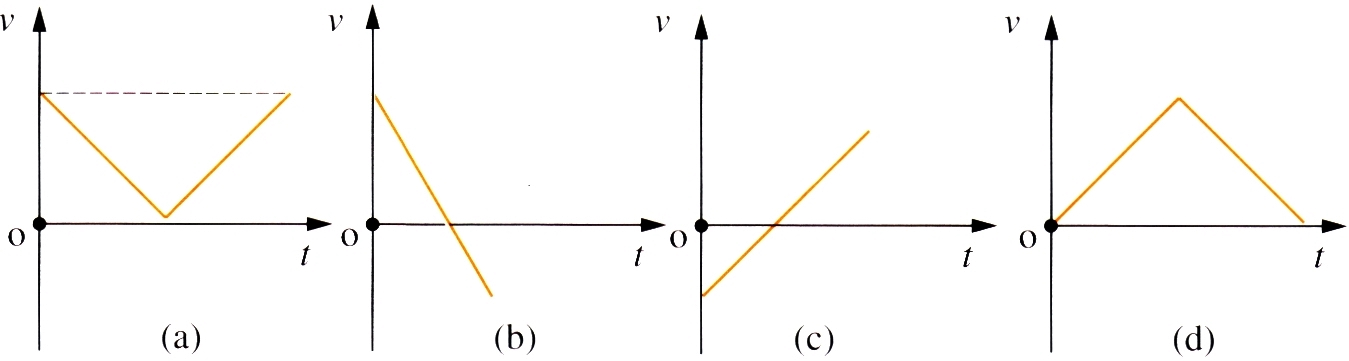
\includegraphics[width=\textwidth]{vw}
	\end{image}
	\begin{oplossing}
		Het juist antwoord is (b). De versnelling is constant waardoor de snelheid lineair moet verlopen in de tijd. Aangezien de referentieas naar boven is gekozen, moet de snelheid in het naar boven bewegen positief zijn. Dat is het geval bij (b).
	\end{oplossing}
\end{exercise}

\begin{exercise}
	Vanaf een klif laat men vanop dezelfde hoogte twee identieke bollen vallen. Men laat de tweede bol \'e\'en seconde later vallen dan de eerste. De luchtwrijving is \textit{niet} te verwaarlozen. Dan
	\begin{multipleChoice}
		\choice{zal de tweede bol iets later dan \'e\'en seconde na de eerste neerkomen.}
		\choice{zal de tweede bol iets vroeger dan \'e\'en seconde na de eerste neerkomen.}
		\choice[correct]{zal de tweede bol exact \'e\'en seconde na de eerste neerkomen.}
		\choice{kunnen we hieromtrent geen uitspraak doen bij gebrek aan gegevens.}
	\end{multipleChoice}
	\begin{oplossing}
		Voor beide bollen is de omstandigheid waarin ze vallen gelijk.
	\end{oplossing}
\end{exercise}

\begin{exercise}
	Vanop een grote hoogte laat men achtereenvolgens twee stenen vallen met een tussentijd van 2 seconden. Op welke wijze verandert de afstand tussen beide stenen in de tijdsduur dat beide vallen?
	\begin{hint}
		Begin met een grafische voorstelling.
	\end{hint}
	\begin{oplossing}
		De afstand verandert lineair in functie van de tijd: $\Delta x(t)=gt_0\cdot t-\frac{1}{2}gt_0^2$ ($=\frac{1}{2}gt^2-\frac{1}{2}g(t-t_0)^2$ met $t\geq t_0=\SI{2}{s}$)
	\end{oplossing}
\end{exercise}

\end{document}
